\documentclass[12pt]{article}

\usepackage[left=3cm, right=3cm]{geometry}
\usepackage{natbib}
\usepackage{tabularx, booktabs, tabulary, array, graphicx, url}
\usepackage{svg}
\usepackage{multirow}
\usepackage{caption}
\usepackage{indentfirst}
\usepackage{subfig}
\usepackage{listings} 
\usepackage{hyperref}
\usepackage{import}
\usepackage{float} 
\usepackage[normalem]{ulem} 

\title{\textbf{Volontariato - DoIT\\[2ex]}
        The Singleton Squad
    }
\author{\textbf{Daniele Buser}\\
    Matricola: 894514\\
    Email: d.buser@campus.unimib.it\\[2ex]
\textbf{Gabriele Groppo}\\
    Matricola: 902238\\
    Email: g.groppo@campus.unimib.it\\[2ex]
\textbf{Andrea Cozzi}\\
    Matricola: 899627\\
    Email: a.cozzi25@campus.unimib.it\\[2ex]
\textbf{Matteo Cervini}\\
    Matricola: 902225\\
    Email: m.cervini1@campus.unimib.it\\
}
\date{26 Gennaio, 2025
    \begin{figure}[H]
        \centering
        
\includegraphics[width=0.3\textwidth]{Immagini/Logo/icon.png}
    \end{figure}
}

\begin{document}

\maketitle

\newpage
\tableofcontents 
\newpage

\section*{\Huge \textbf{Introduzione}}
\addcontentsline{toc}{section}{Introduzione}
\setcounter{subsection}{0} 
\renewcommand{\thesubsection}{\arabic{subsection}} 

\import{Introduzione/}{Introduzione.tex}

\section*{\Huge \textbf{Compilazione}}
\addcontentsline{toc}{section}{Compilazione}
\setcounter{subsection}{0} 
\renewcommand{\thesubsection}{\arabic{subsection}} 

Per compilare il progetto sono necessari i seguenti passaggi:
\begin{enumerate}
    \item {\textbf{E' necessario installare npm, nextJS e react}}: per farlo è necessario eseguire il comando {\textbf{npm install -g next react}}.
    \item {\textbf{npm install}}: per installare le dipendenze necessaricreare la build del progetto.
    \item {\textbf{npm run dev}}: per avviare il server Frontend, è necessario entrare nella cartella: /frontend/doit/.
    \item {\textbf{`mvn clean install`}}: per avviare il server backend, è necessario entrare nella cartella: /backend/doit/.
    \item {\textbf{`mvn spring-boot:run`}}: per avviare il server backend, è necessario entrare nella cartella: /backend/doit/.
\end{enumerate}

\section*{\Huge \textbf{Iterazione 1}}
\addcontentsline{toc}{section}{Iterazione 1}
\setcounter{subsection}{0} 
\renewcommand{\thesubsection}{\arabic{subsection}} 

\section{Diagramma di Gantt}
Questi sono i diagrammi di Gantt per l'iterazione 2.

\begin{figure}[H]
    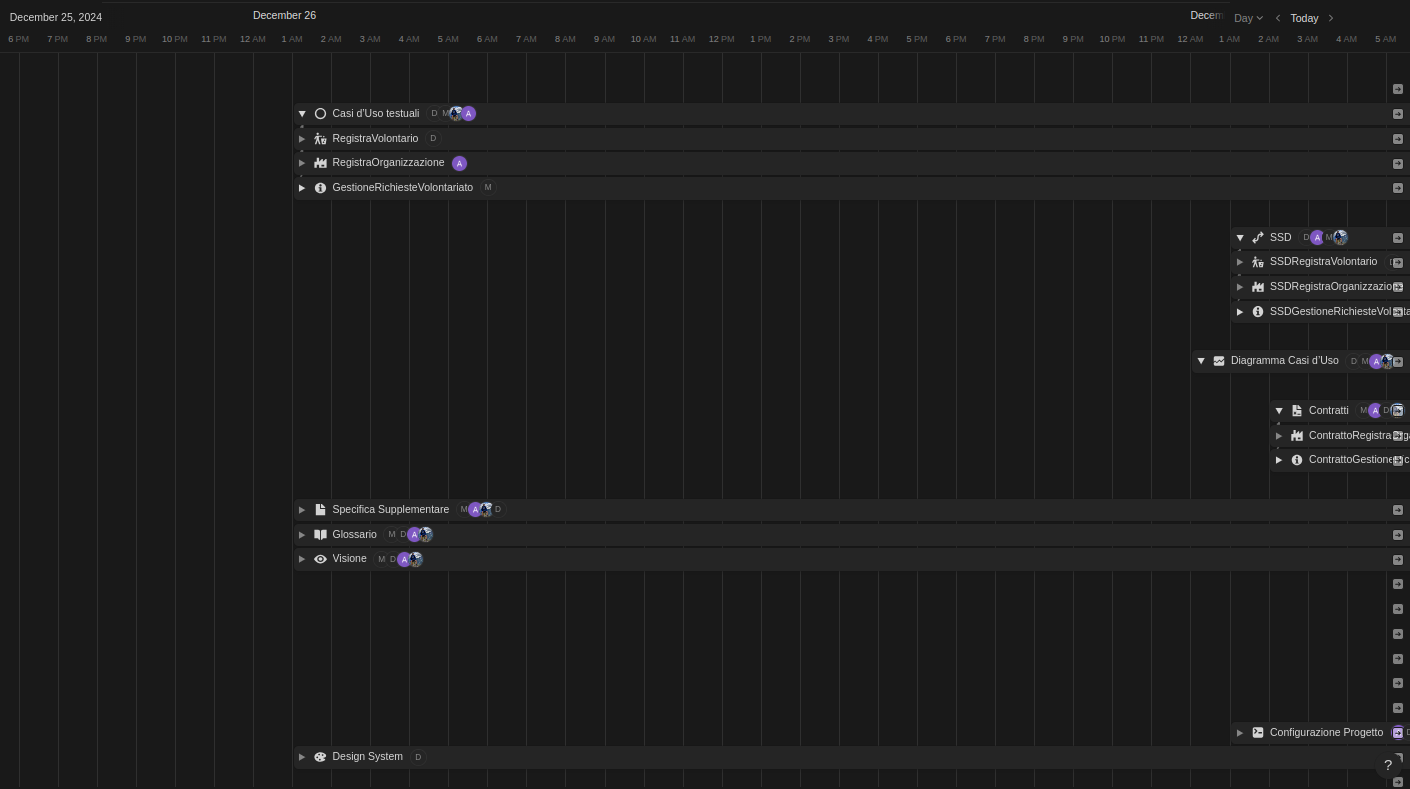
\includegraphics[width=\textwidth,keepaspectratio]{Immagini/Gantt/Iterazione 1/Gantt1.png}
        \caption{Diagramma di Gantt 1} 
        \label{fig:Gantt1}
\end{figure}

\begin{figure}[H]
    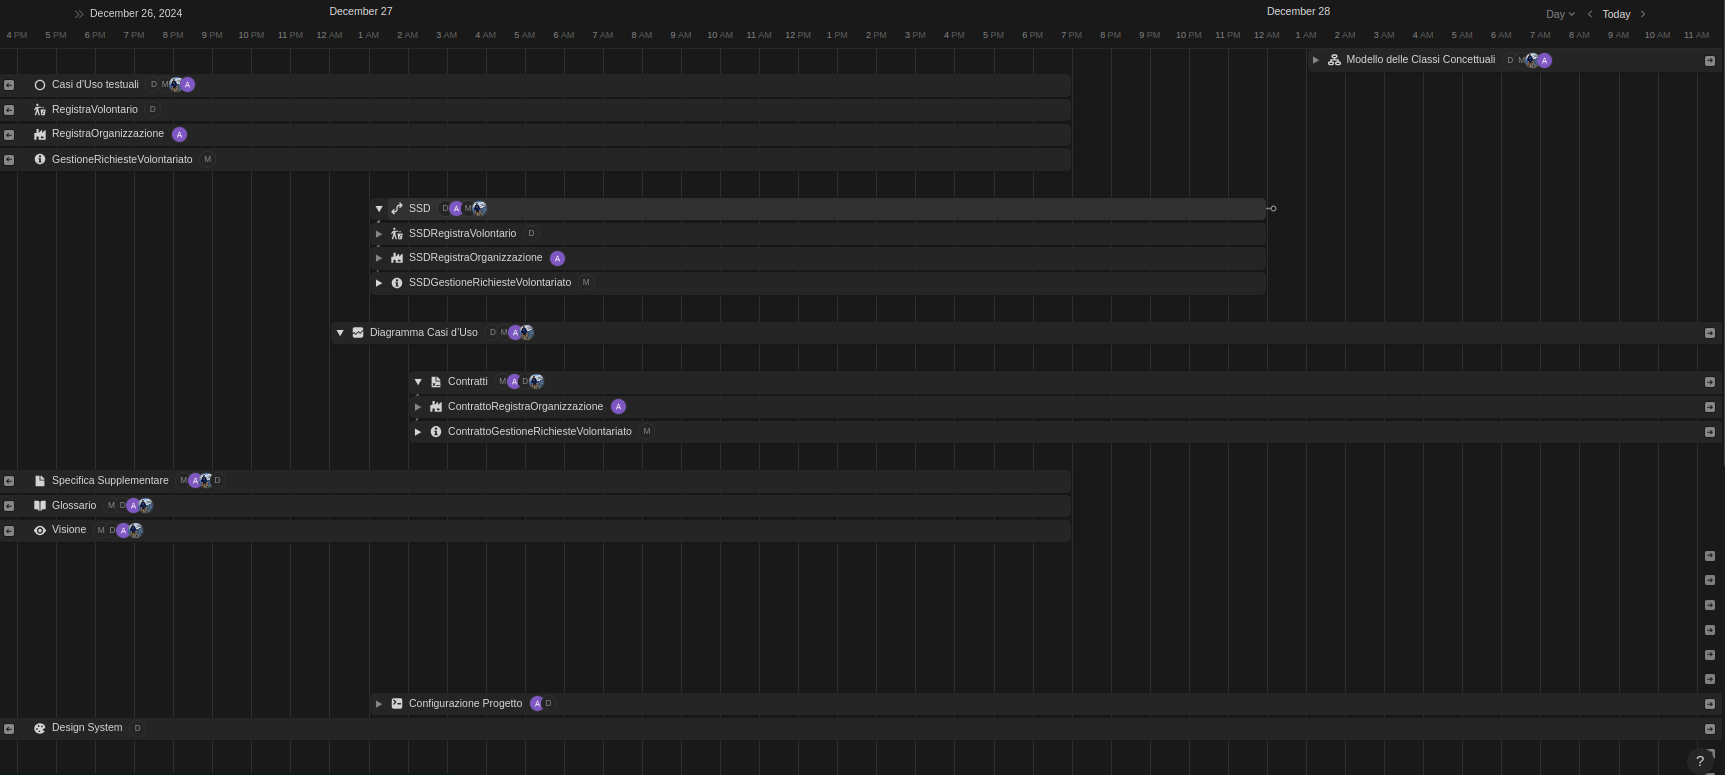
\includegraphics[width=\textwidth,keepaspectratio]{Immagini/Gantt/Iterazione 1/Gantt2.png}
        \caption{Diagramma di Gantt 2} 
        \label{fig:Gantt2}
\end{figure}

\begin{figure}[H]
    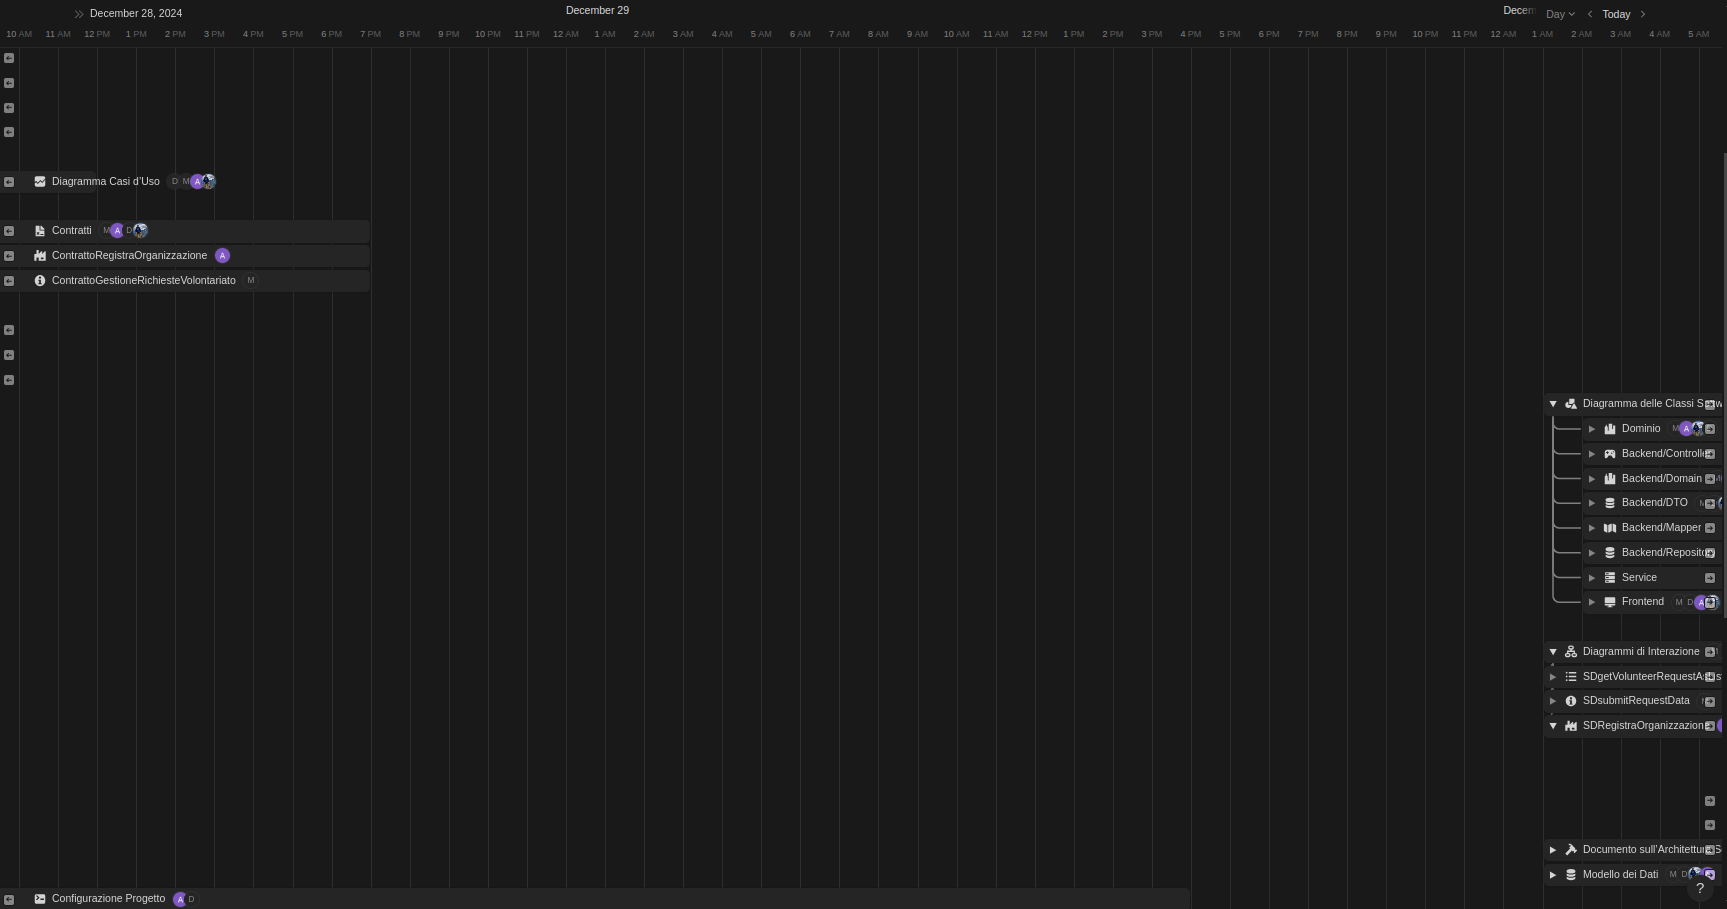
\includegraphics[width=\textwidth,keepaspectratio]{Immagini/Gantt/Iterazione 1/Gantt3.png}
        \caption{Diagramma di Gantt 3} 
        \label{fig:Gantt3}
\end{figure}

\begin{figure}[H]
    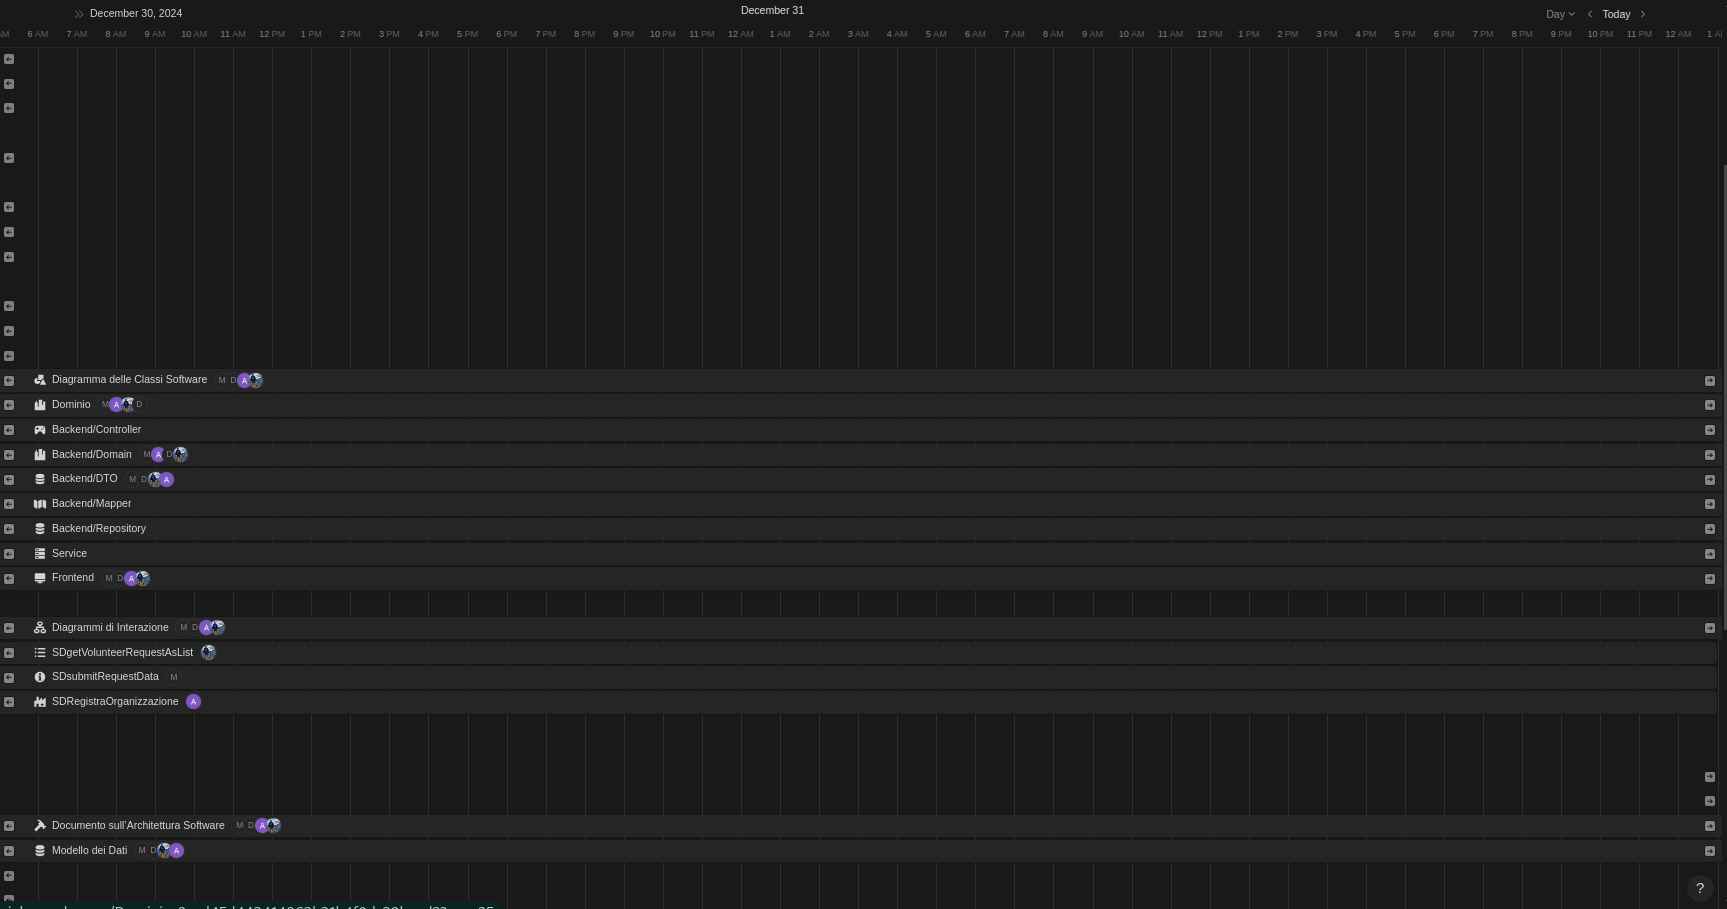
\includegraphics[width=\textwidth,keepaspectratio]{Immagini/Gantt/Iterazione 1/Gantt4.png}
        \caption{Diagramma di Gantt 4} 
        \label{fig:Gantt4}
\end{figure}

\begin{figure}[H]
    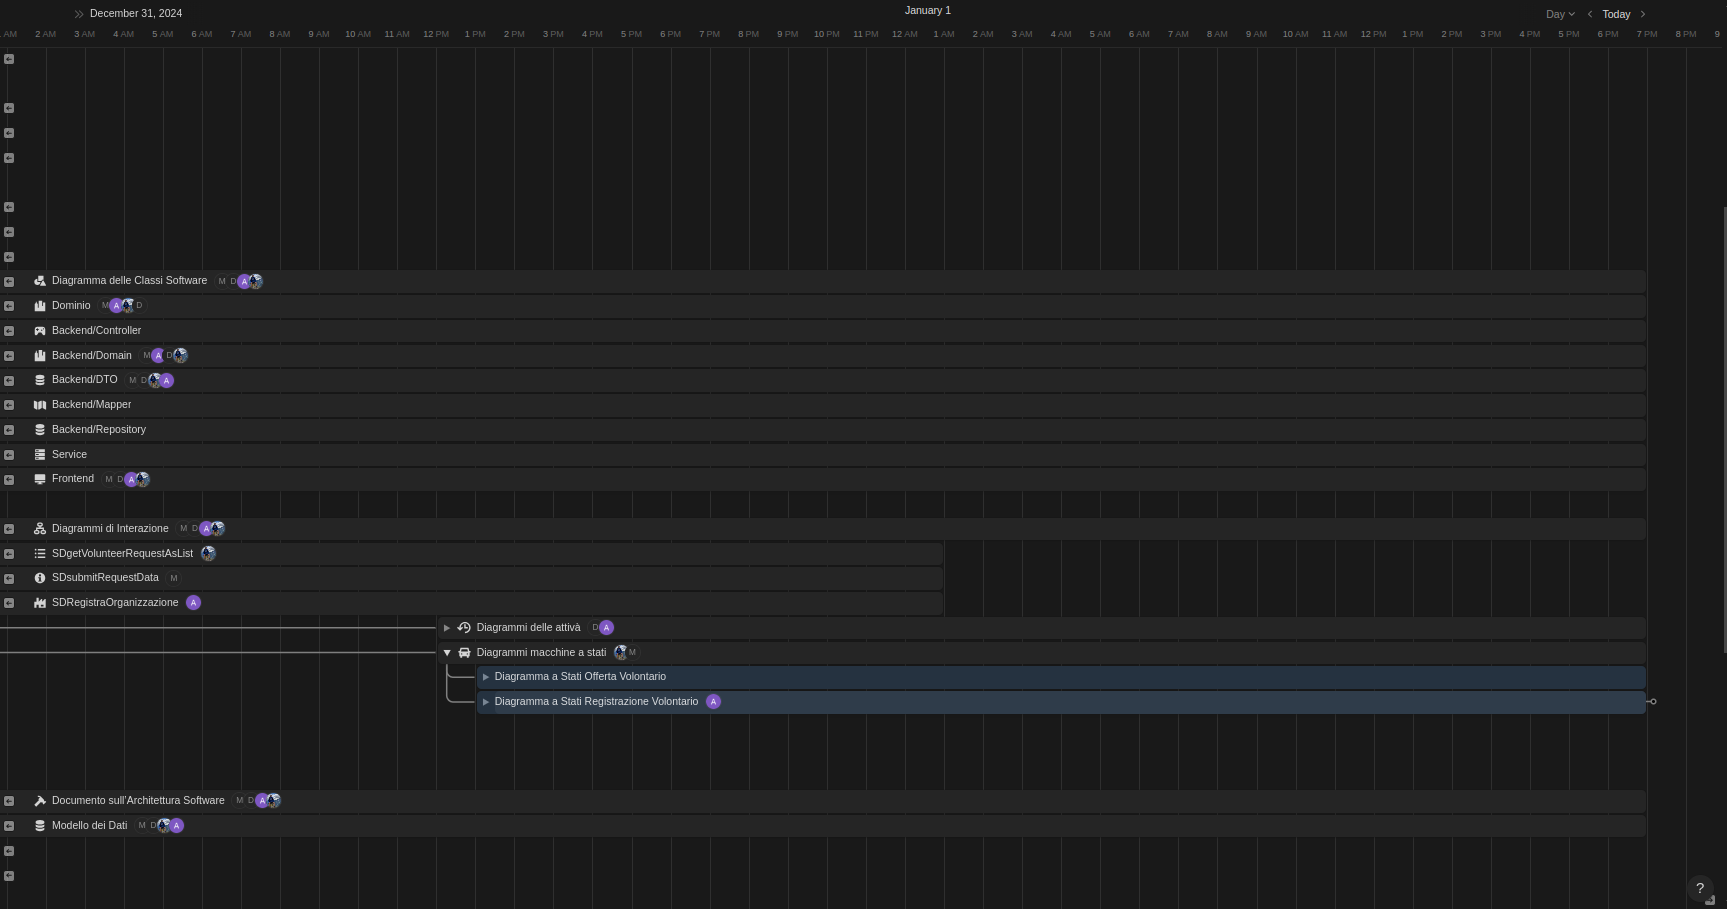
\includegraphics[width=\textwidth,keepaspectratio]{Immagini/Gantt/Iterazione 1/Gantt5.png}
        \caption{Diagramma di Gantt 5} 
        \label{fig:Gantt5}
\end{figure}

\begin{figure}[H]
    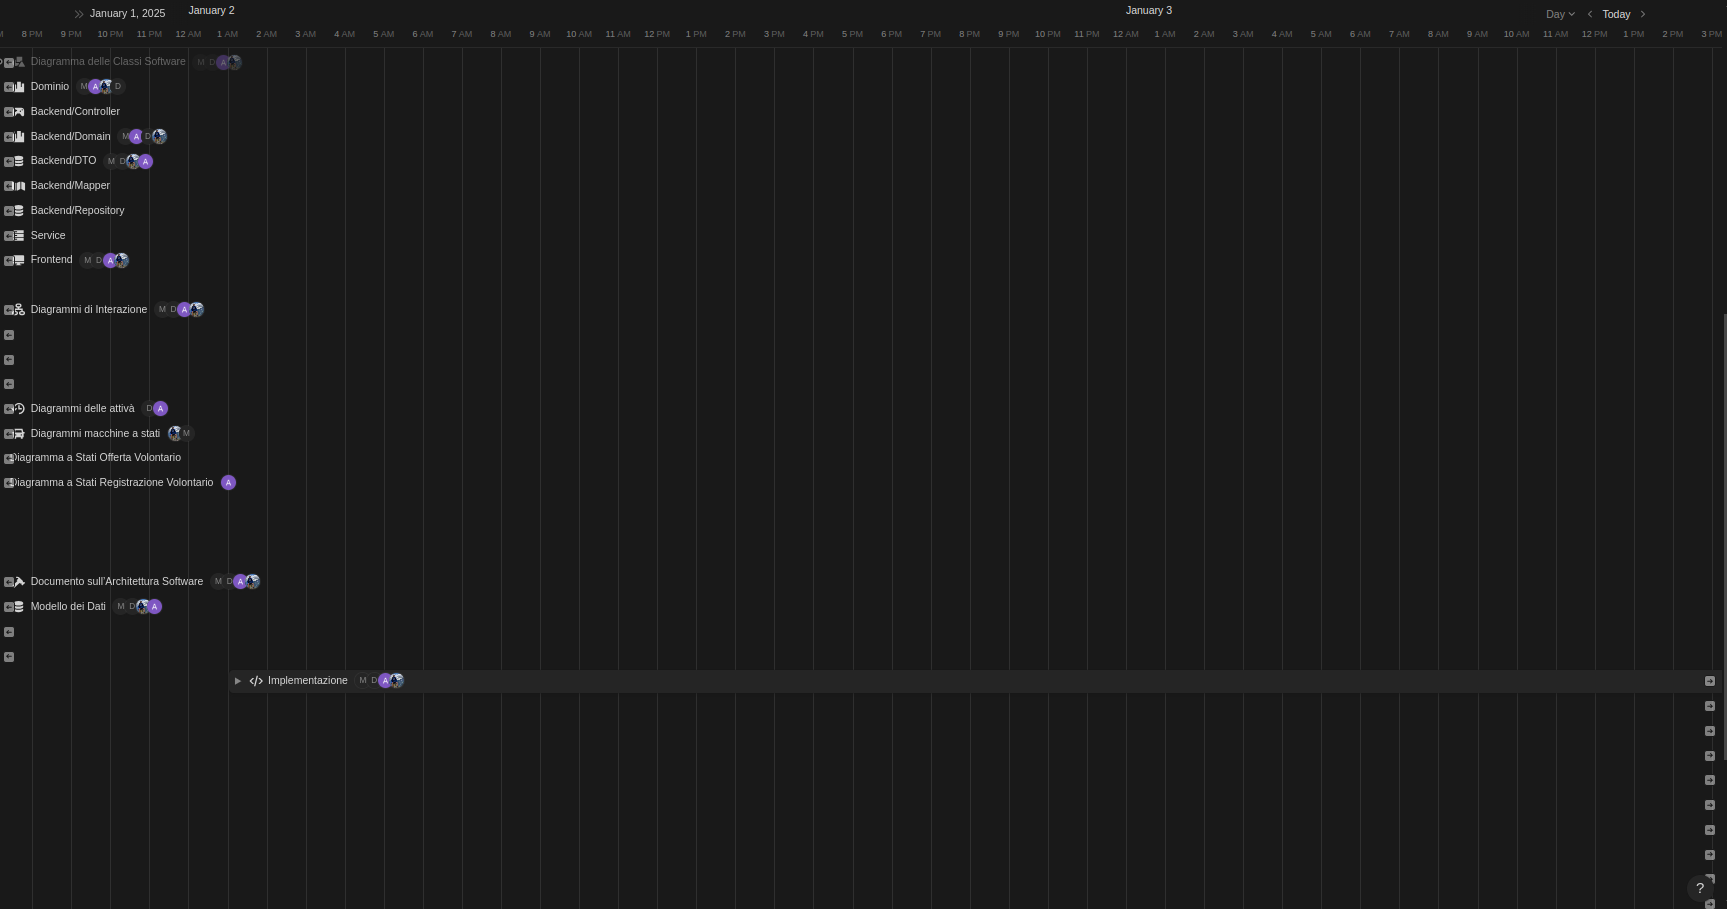
\includegraphics[width=\textwidth,keepaspectratio]{Immagini/Gantt/Iterazione 1/Gantt6.png}
        \caption{Diagramma di Gantt 6} 
        \label{fig:Gantt6}
\end{figure}

\begin{figure}[H]
    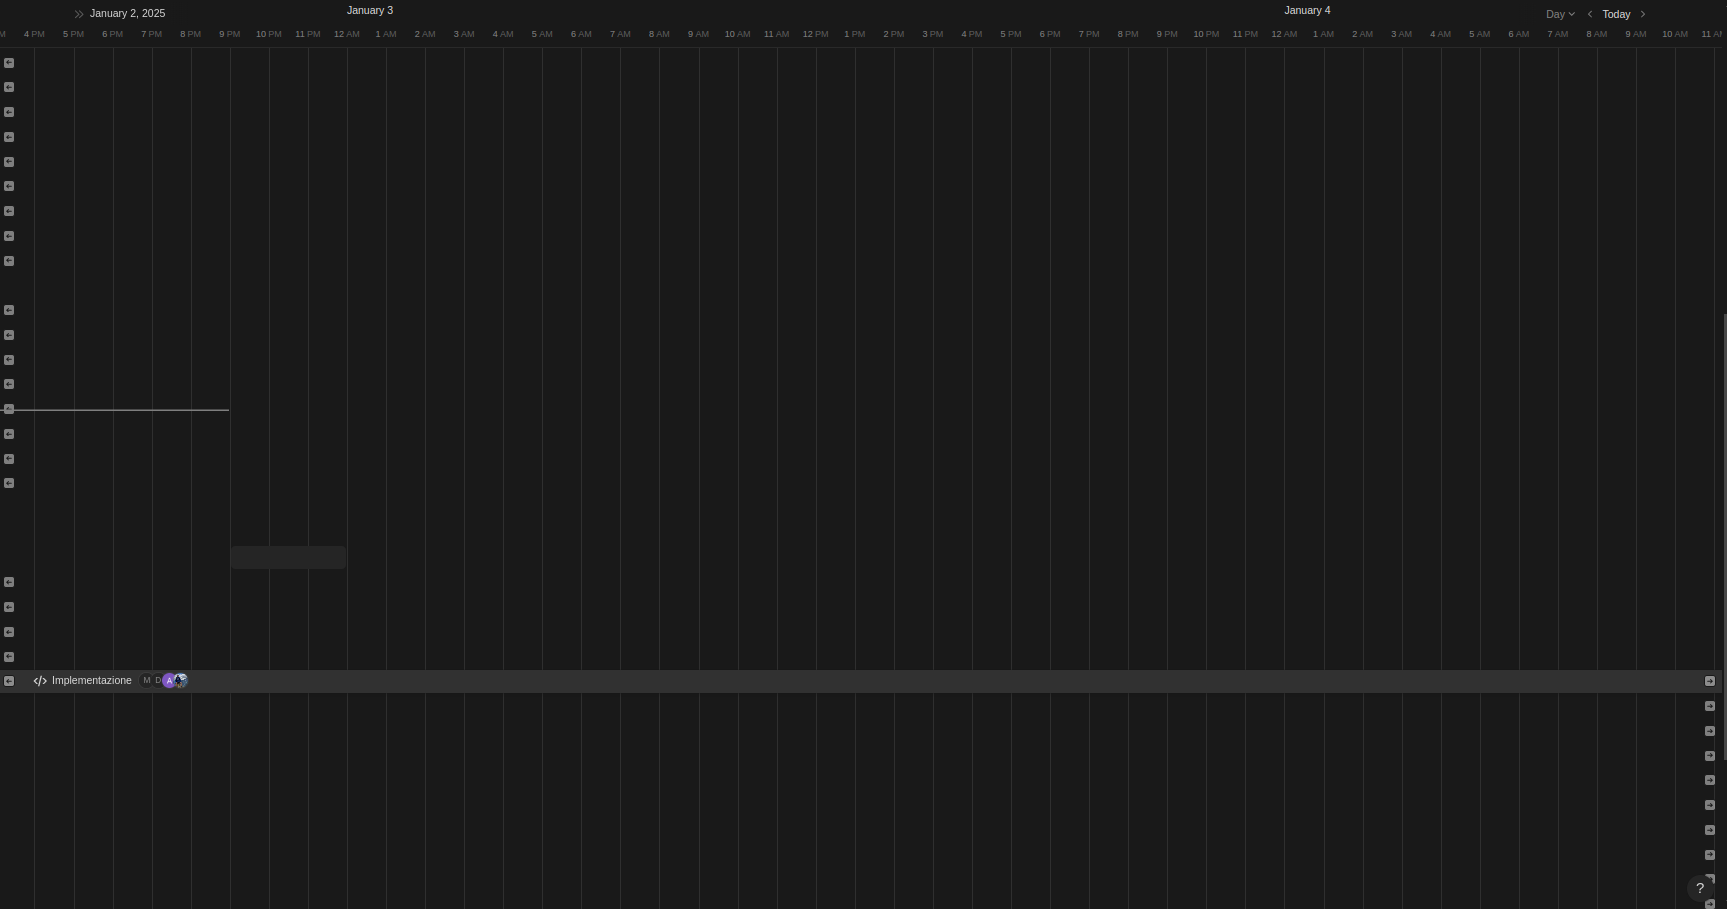
\includegraphics[width=\textwidth,keepaspectratio]{Immagini/Gantt/Iterazione 1/Gantt7.png}
        \caption{Diagramma di Gantt 7} 
        \label{fig:Gantt7}
\end{figure}

\begin{figure}[H]
    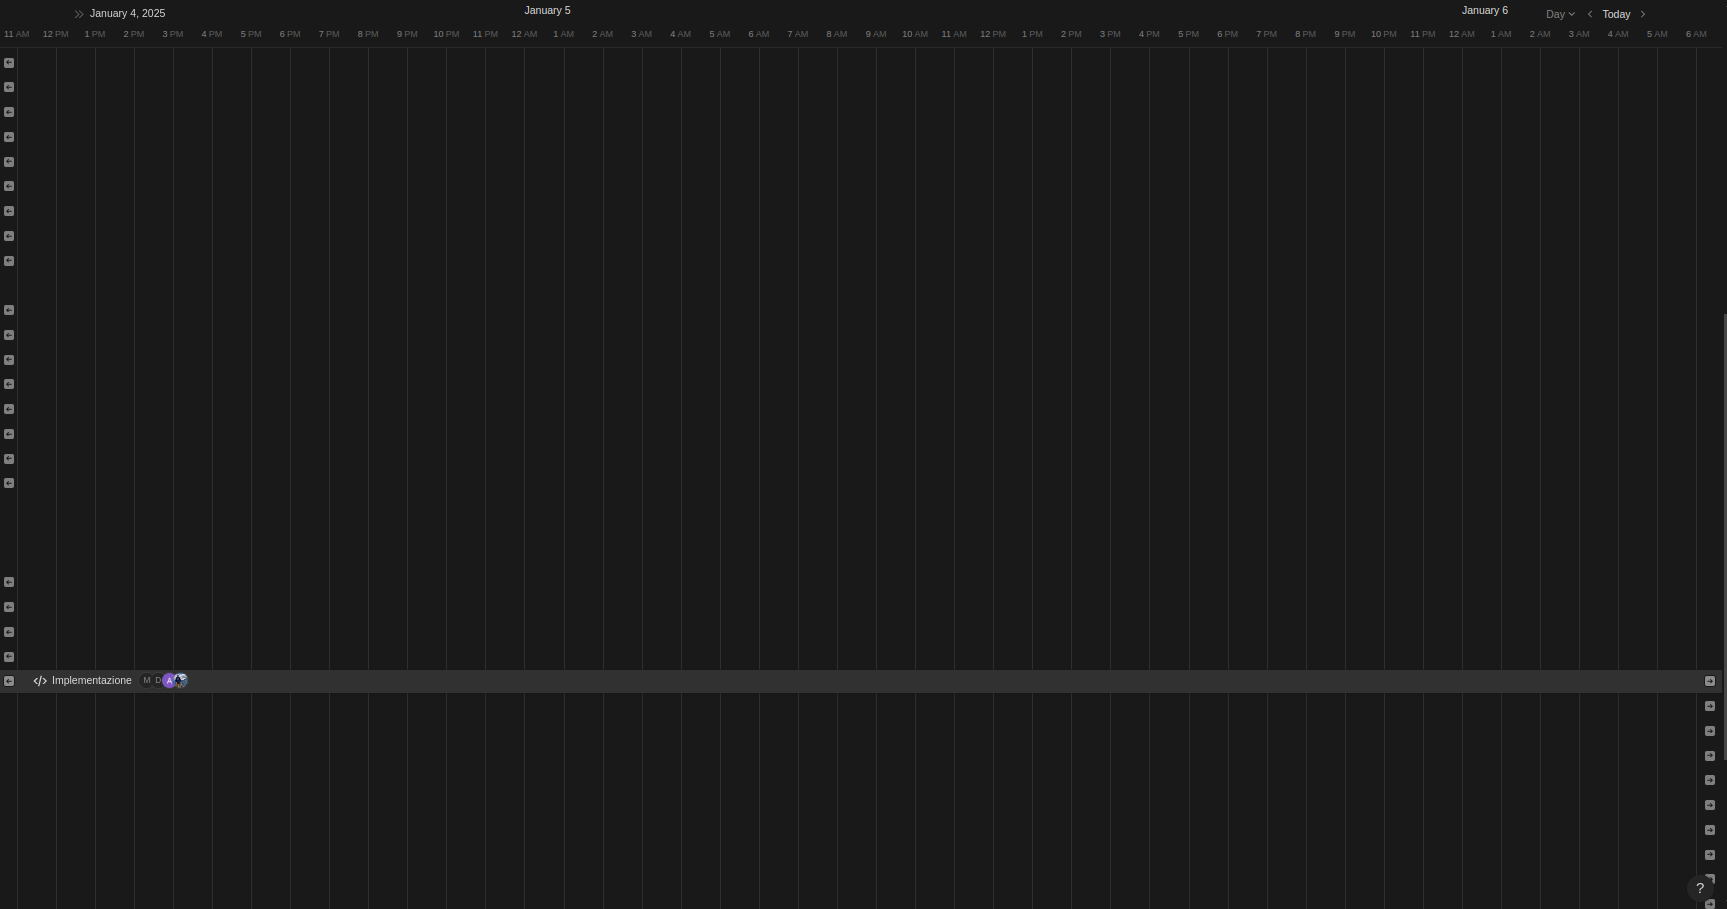
\includegraphics[width=\textwidth,keepaspectratio]{Immagini/Gantt/Iterazione 1/Gantt8.png}
        \caption{Diagramma di Gantt 8} 
        \label{fig:Gantt8}
\end{figure}

\begin{figure}[H]
    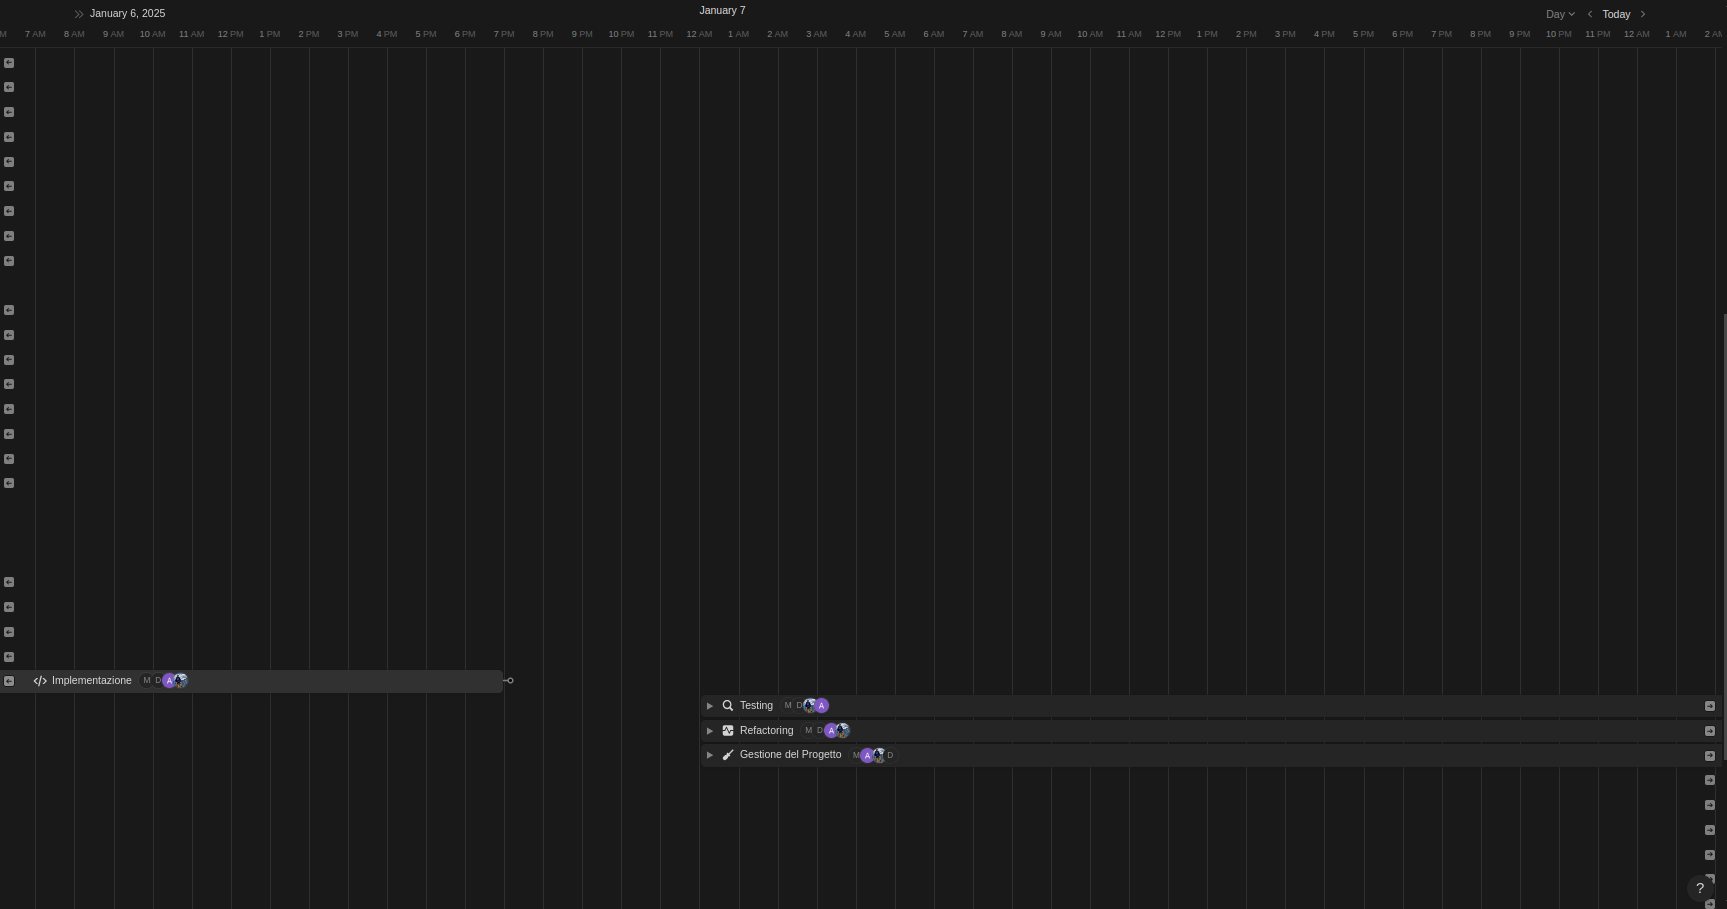
\includegraphics[width=\textwidth,keepaspectratio]{Immagini/Gantt/Iterazione 1/Gantt9.png}
        \caption{Diagramma di Gantt 9} 
        \label{fig:Gantt9}
\end{figure}

\begin{figure}[H]
    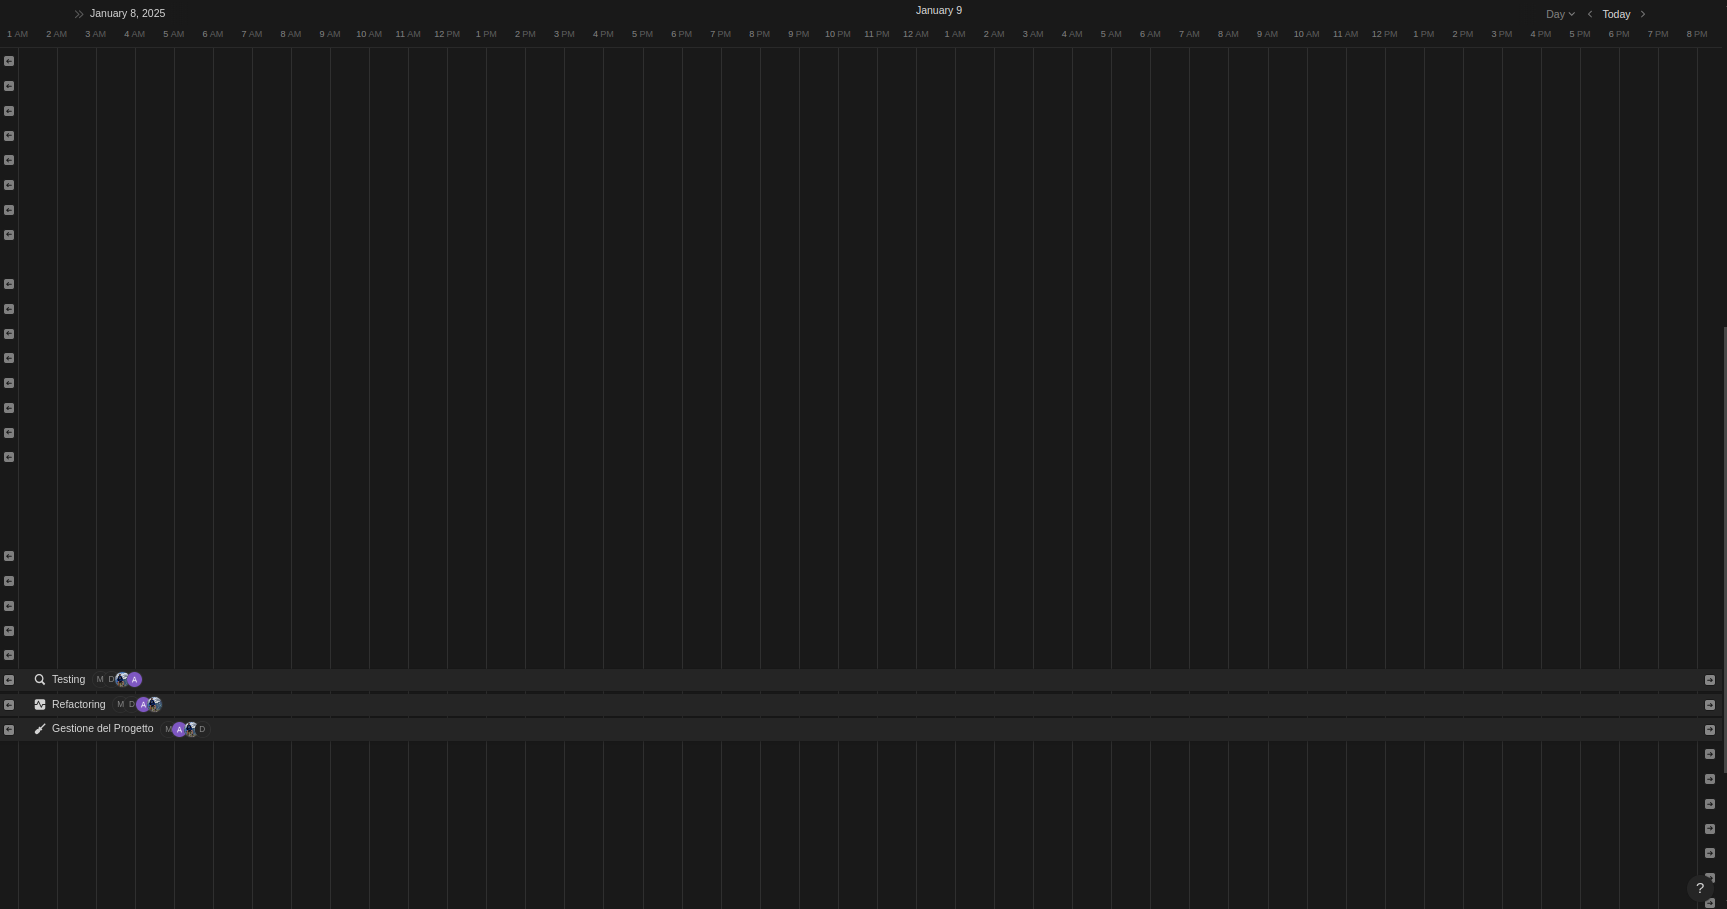
\includegraphics[width=\textwidth,keepaspectratio]{Immagini/Gantt/Iterazione 1/Gantt10.png}
        \caption{Diagramma di Gantt 10} 
        \label{fig:Gantt10}
\end{figure}

\begin{figure}[H]
    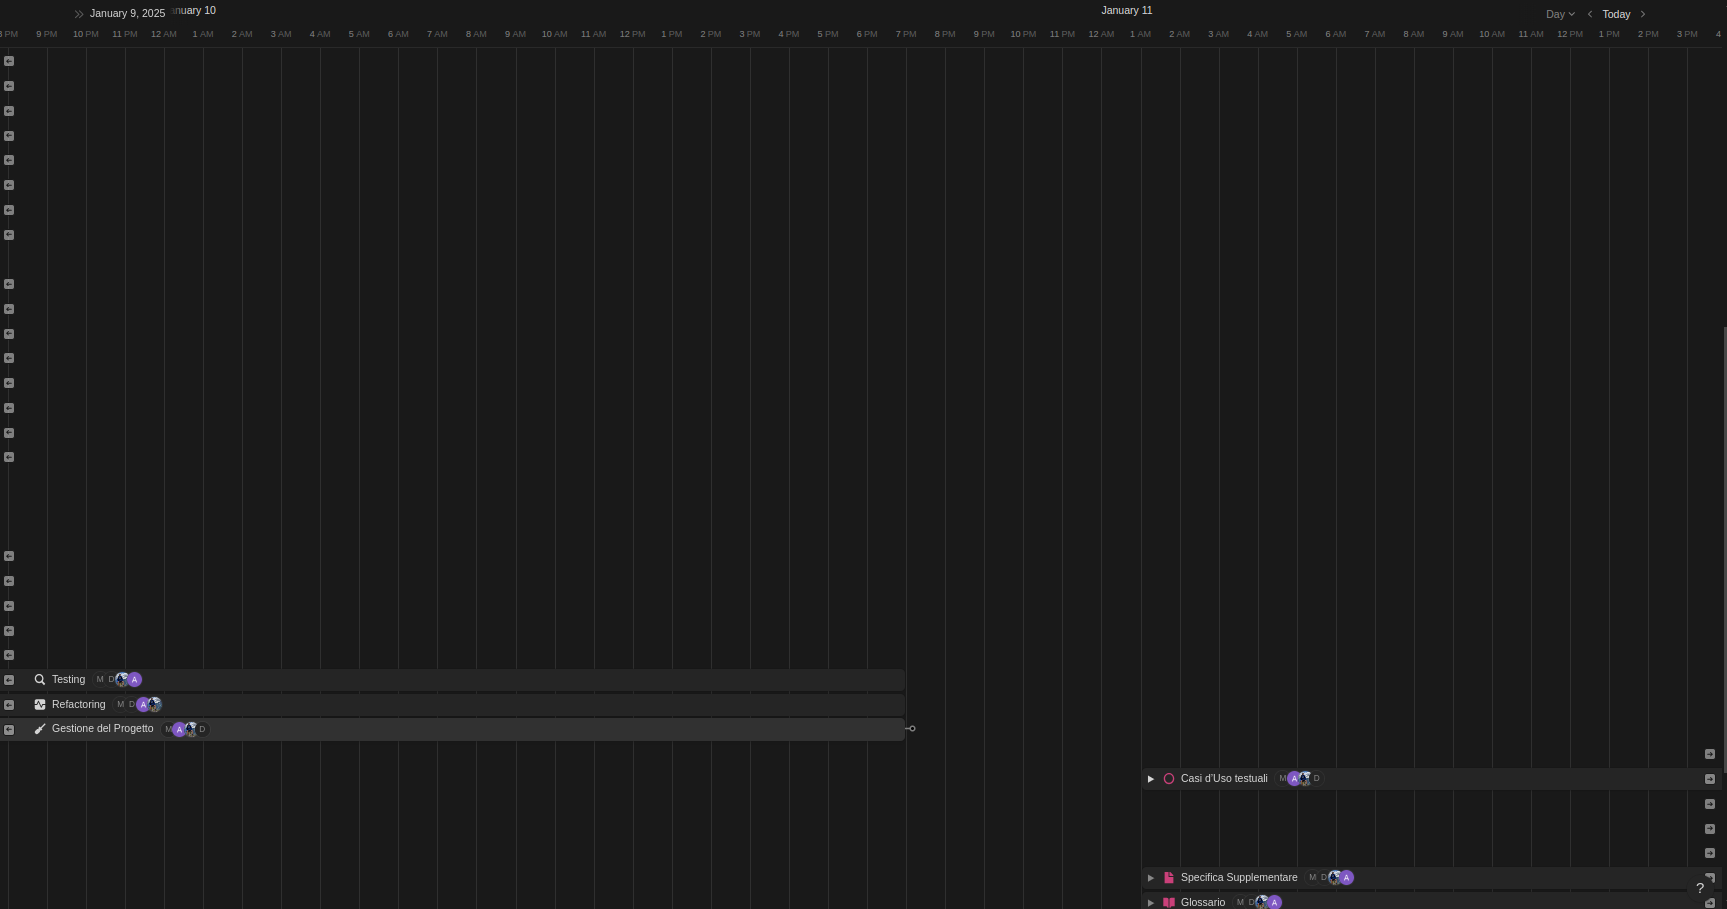
\includegraphics[width=\textwidth,keepaspectratio]{Immagini/Gantt/Iterazione 1/Gantt11.png}
        \caption{Diagramma di Gantt 11} 
        \label{fig:Gantt11}
\end{figure}


\section{Requisiti}
\subsection{Casi d'uso}

\subsubsection{Caso d'uso UC1: RegistraVolontario}
\import{CasiD'uso/Iterazione 1/}{RegistraVolontario.tex}

\subsubsection{Caso d'uso UC2: RegistraOrganizzazione}
\import{CasiD'uso/Iterazione 1/}{RegistraOrganizzazione.tex}

\subsubsection{Caso d'uso UC3: GestioneRichiesteVolontariato}
\import{CasiD'uso/Iterazione 1/}{GestioneRichiesteVolontariato.tex}

\subsection{Diagramma dei Casi d'Uso}
\import{Immagini/DiagrammaDeiCasiD'Uso/Iterazione 1/}{Diagramma.tex}
\begin{figure}[H]
    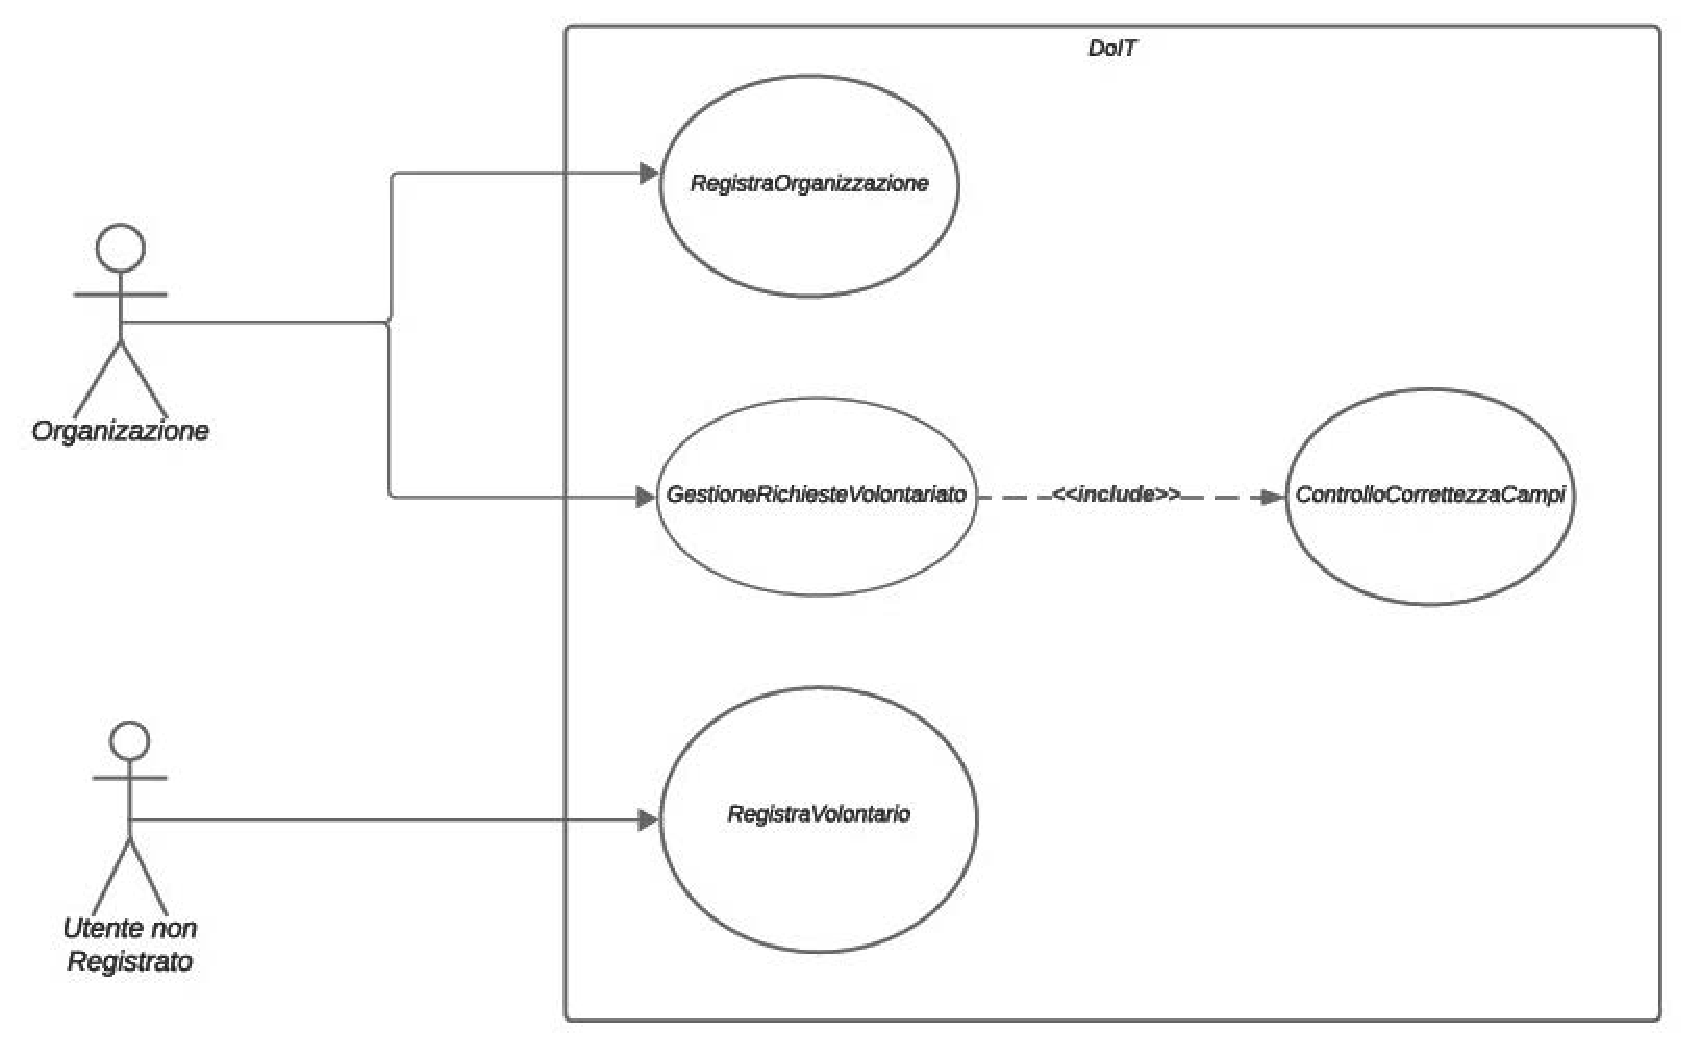
\includegraphics[width=\textwidth,keepaspectratio]{Immagini/DiagrammaDeiCasiD'Uso/Iterazione 1/Diagramma.pdf}
        \caption{Diagramma dei Casi d'Uso}
        \label{fig:diagrammaCasiUso1}
\end{figure}

\subsection{Diagramma di Sequenza di Sistema}
\subsubsection{Diagramma di Sequenza di Sistema SSD1: RegistraVolontario}

\import{Immagini/SSD/Iterazione 1/}{RegistraVolontario.tex}

\begin{figure}[H]
    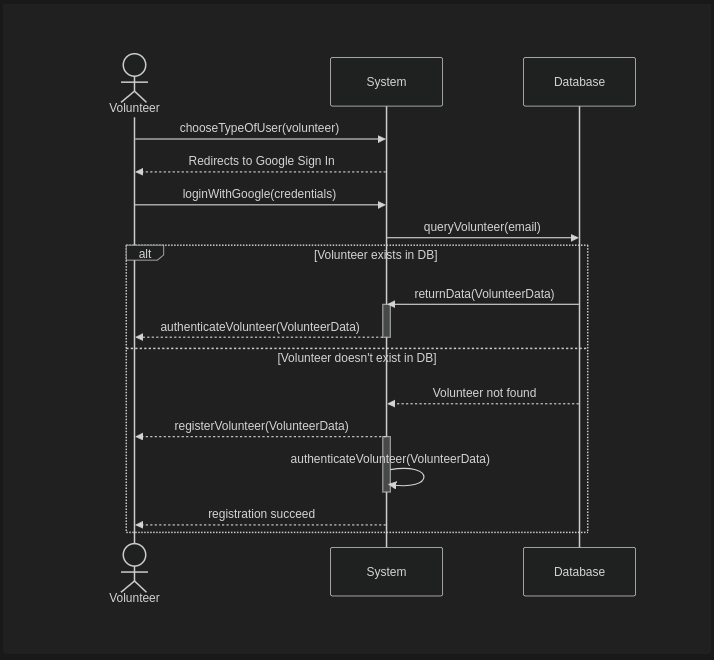
\includegraphics[width=\textwidth, keepaspectratio]{Immagini/SSD/Iterazione 1/SSDRegistraVolontario.png}
        \caption{Diagramma di Sequenza di Sistema}
        \label{fig:diagrammaSSD1}
\end{figure}

\subsubsection{Diagramma di Sequenza di Sistema SSD2: RegistraOrganizzazione}

\import{Immagini/SSD/Iterazione 1/}{RegistraOrganizzazione.tex}

\begin{figure}[H]
    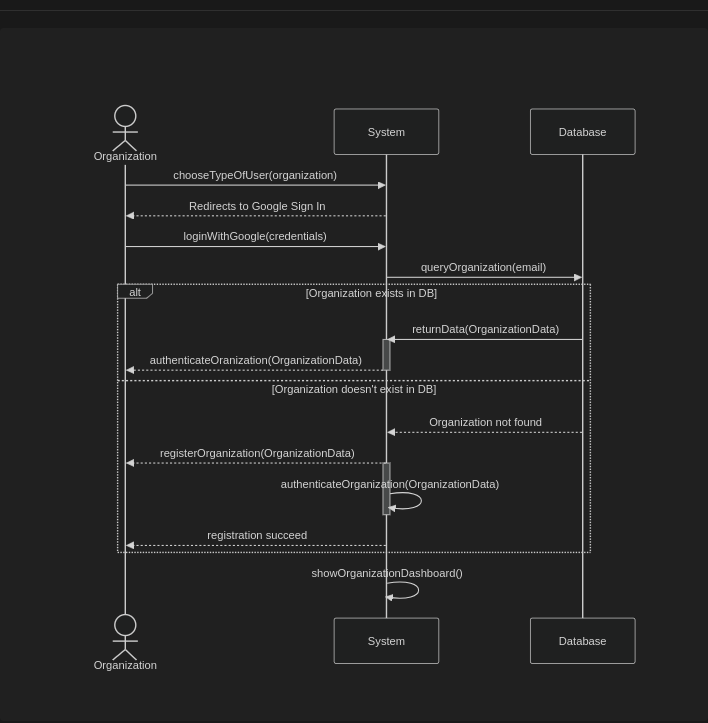
\includegraphics[width=\textwidth,keepaspectratio]{Immagini/SSD/Iterazione 1/SSDRegistraOrganizzazione.png}
        \caption{Diagramma di Sequenza di Sistema}
        \label{fig:diagrammaSSD2}
\end{figure}

\subsubsection{Diagramma di Sequenza di Sistema SSD3: GestioneRichiesteVolontariato}

\import{Immagini/SSD/Iterazione 1/}{GestioneRichiesteVolontariato.tex}

\begin{figure}[H]
    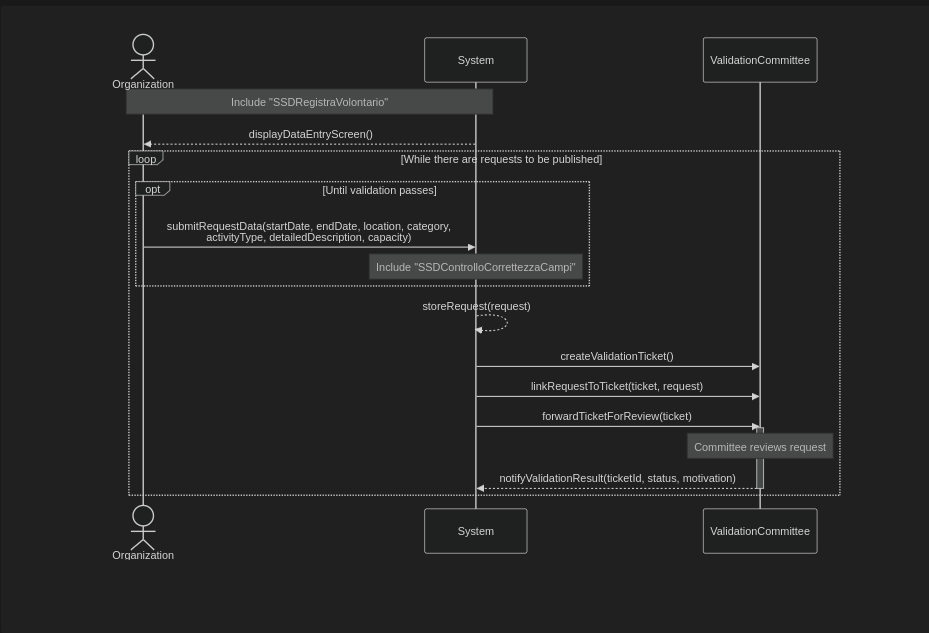
\includegraphics[width=\textwidth,keepaspectratio]{Immagini/SSD/Iterazione 1/SSDGestioneRichiesteVolontariato.png}
        \caption{Diagramma di Sequenza di Sistema}
        \label{fig:diagrammaSSD3}
\end{figure}

\subsubsection{Diagramma di Sequenza di Sistema SSD3.2: ControlloCorrettezzaCampi}

\import{Immagini/SSD/Iterazione 1/}{ControlloCorrettezzaCampi.tex}

\begin{figure}[H]
    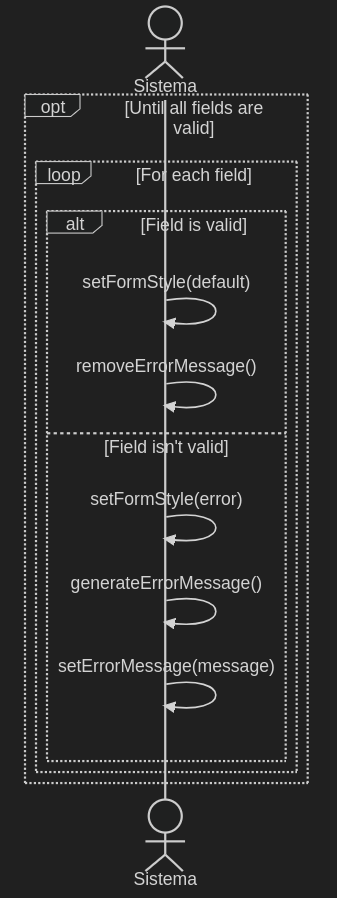
\includegraphics[width=\textwidth, height=0.5\textheight,keepaspectratio]{Immagini/SSD/Iterazione 1/SSDControlloCorrettezzaCampi.png}
        \caption{Diagramma di Sequenza di Sistema}
        \label{fig:diagrammaSSD3.2}
\end{figure}

\subsection{Contratti}
\subsubsection{Contratto CO01: RegistraOrganizzazione}
\import{Contratti/Iterazione 1/}{RegistraOrganizzazione.tex}

\subsubsection{Contratto CO02: GestioneRichiesteVolontariato}
\import{Contratti/Iterazione 1/}{GestioneRichiesteVolontariato.tex}

\subsubsection{Contratto CO02.2: ControlloCorrettezzaCampi}
\import{Contratti/Iterazione 1/}{ControlloCorrettezzaCampi.tex}

\subsection{Specifica Supplementare}
\import{ArtefattiSupplementari/Iterazione 1/}{SpecificaSupplementare.tex}

\subsection{Glossario}
\import{ArtefattiSupplementari/Iterazione 1/}{Glossario.tex}

\subsection{Visione}
\import{ArtefattiSupplementari/Iterazione 1/}{Visione.tex}

\section{Modellazione di Business}
\subsection{Modello delle Classi Concettuali}

\import{Immagini/ModellazioneDiBusiness/Iterazione 1/}{Diagramma.tex}
\begin{figure}[H]
    \includegraphics[width=1.17\textwidth, height=\textheight,keepaspectratio]{Immagini/ModellazioneDiBusiness/Iterazione 1/Diagramma.png}
        \caption{Modello delle Classi Concettuali}
        \label{fig:Modello delle Classi Concettuali 1}
\end{figure}

\section{Progettazione}
\subsection{Diagrammi d'Interazione}

\subsubsection{Diagramma di Sequenza SD1: RegisterOrganization}
\import{Immagini/SD/Iterazione 1/}{RegistraOrganizzazione.tex}

\begin{figure}[H]
    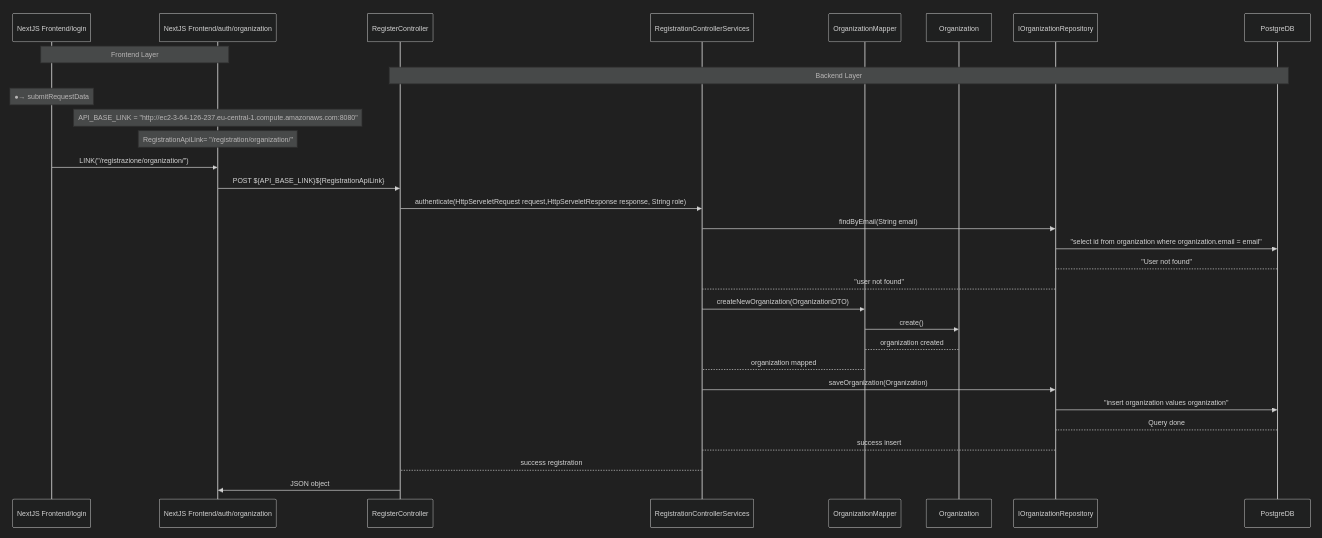
\includegraphics[width=\textwidth, height=\textheight,keepaspectratio]{Immagini/SD/Iterazione 1/SDRegistraOrganizzazione.png}
        \caption{Diagramma di Interazione}
        \label{fig:diagrammaSD1}
\end{figure}

\subsubsection{Diagramma di Sequenza SD2: SubmitRequestData}
\import{Immagini/SD/Iterazione 1/}{SubmitRequestData.tex}

\begin{figure}[H]
    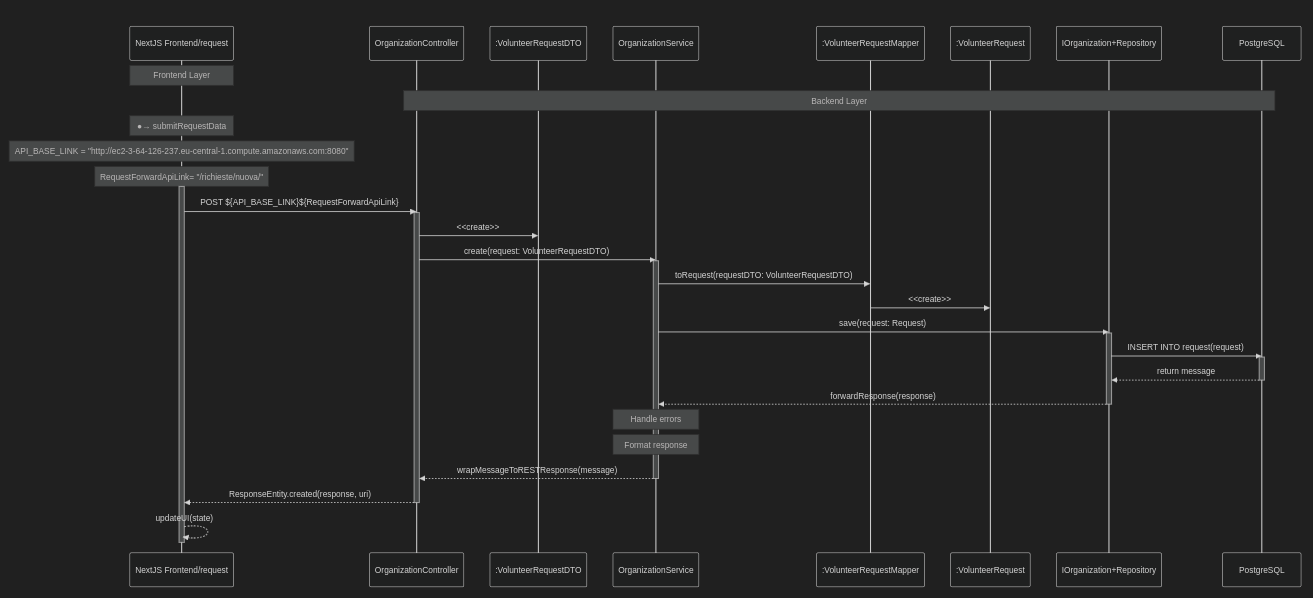
\includegraphics[width=\textwidth, height=\textheight,keepaspectratio]{Immagini/SD/Iterazione 1/SDSubmitRequestData.png}
        \caption{Diagramma di Interazione}
        \label{fig:diagrammaSD2}
\end{figure}

\subsubsection{Diagramma di Sequenza SD3: GetVolunteeRequestAsList}
\import{Immagini/SD/Iterazione 1/}{GetVolunteeRequestAsList.tex}

\begin{figure}[H]
    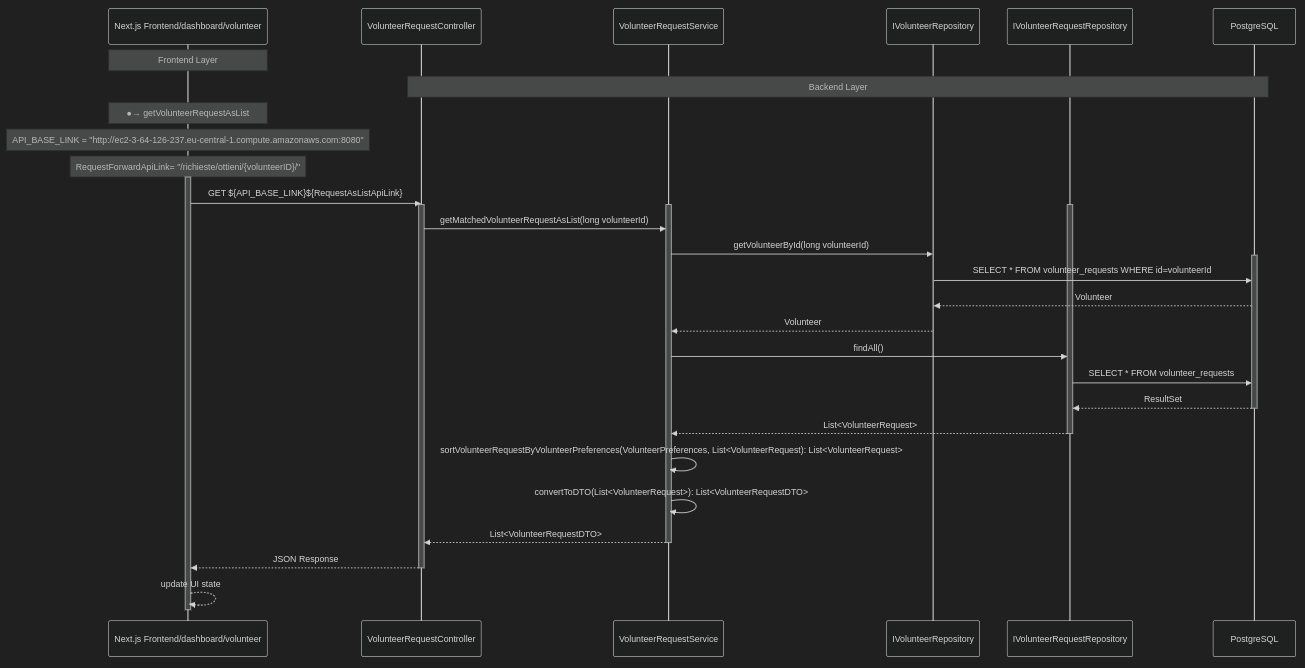
\includegraphics[width=\textwidth, height=\textheight,keepaspectratio]{Immagini/SD/Iterazione 1/SDGetVolunteeRequestAsList.png}
        \caption{Diagramma di Interazione}
        \label{fig:diagrammaSD3}
\end{figure}

\subsection{Diagrammi delle Attività}

\subsubsection{Diagramma delle Attività DA1: SubmitRequest}
\import{Immagini/DA/Iterazione 1/}{SubmitRequest.tex}

\begin{figure}[H]
    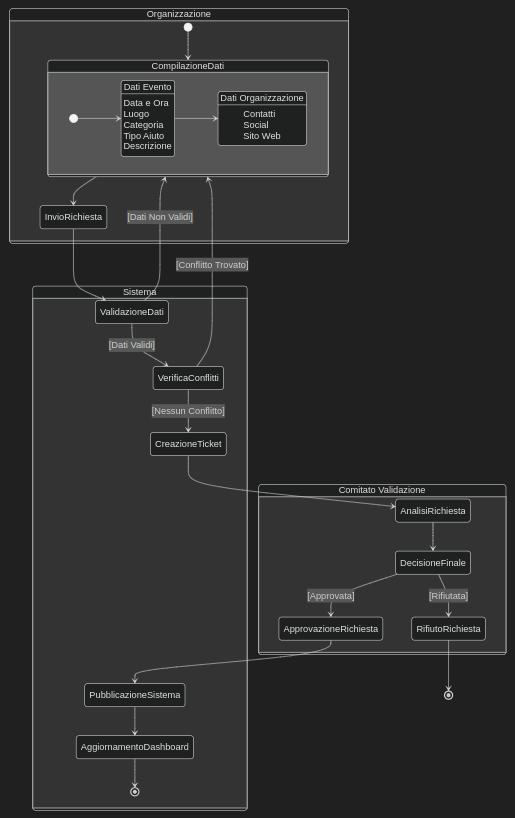
\includegraphics[width=\textwidth, height=\textheight,keepaspectratio]{Immagini/DA/Iterazione 1/SDSubmitRequest.png}
        \caption{Diagramma delle Attività}
        \label{fig:diagrammaDA1}
\end{figure}

\subsection{Diagrammi delle Macchine a Stati}

\subsubsection{Diagramma delle Macchine a Stati DS1: RegisterVolunteer}
\import{Immagini/DS/Iterazione 1/}{RegistrazioneVolontario.tex}

\begin{figure}[H]
    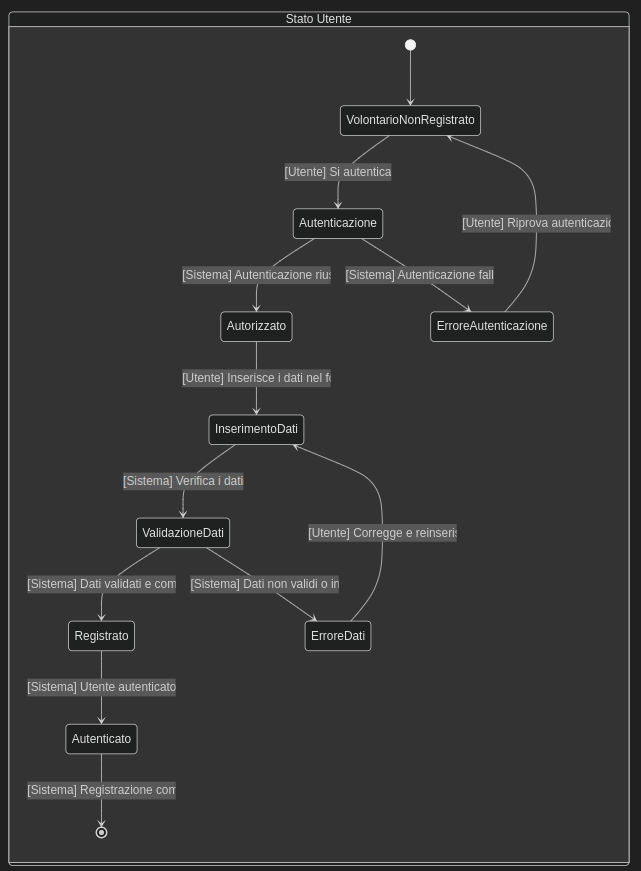
\includegraphics[width=\textwidth, height=\textheight,keepaspectratio]{Immagini/DS/Iterazione 1/DSRegistrazioneVolontario.png}
        \caption{Diagramma delle Attività}
        \label{fig:diagrammaDS1}
\end{figure}

\subsubsection{Diagramma delle Macchine a Stati DS2: VolunteerOffers}
\import{Immagini/DS/Iterazione 1/}{OfferteVolontario.tex}

\begin{figure}[H]
    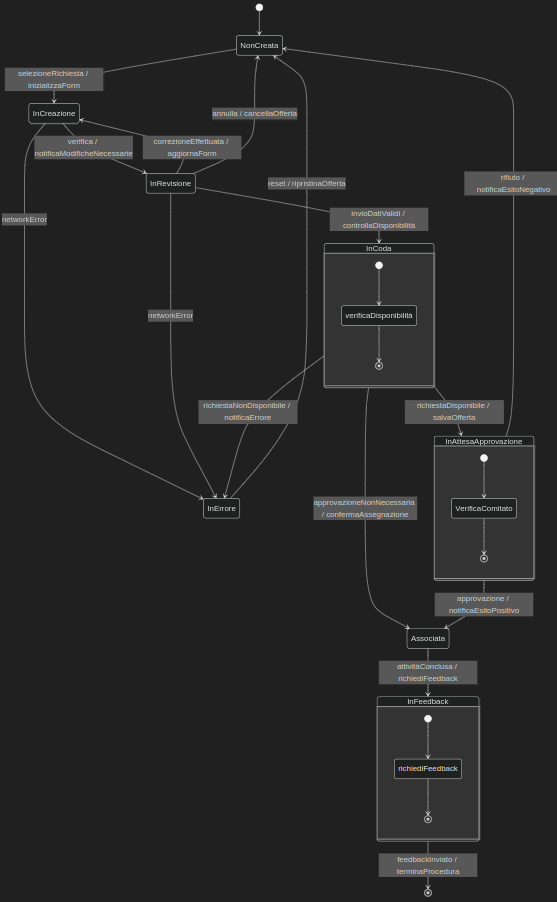
\includegraphics[width=\textwidth, height=\textheight,keepaspectratio]{Immagini/DS/Iterazione 1/DSOfferteVolontario.png}
        \caption{Diagramma delle Attività}
        \label{fig:diagrammaDS2}
\end{figure}

\subsection{Diagrammi delle Classi Software di Progetto}-

\subsubsection{Diagramma delle Classi Software di Progetto DCSP1: Dominio}
\import{Immagini/DCSP/Iterazione 1/}{Domain.tex}

\begin{figure}[H]
    \includegraphics[width=\textwidth, height=\textheight,keepaspectratio]{Immagini/DCSP/Iterazione 1/DCSPDomain.png}
        \caption{Diagramma delle Classi Software di Progetto}
        \label{fig:diagrammaDCSP1}
\end{figure}

\subsubsection{Diagramma delle Classi Software di Progetto DCSP2: Frontend}
\import{Immagini/DCSP/Iterazione 1/}{Frontend.tex}

\begin{figure}[H]
    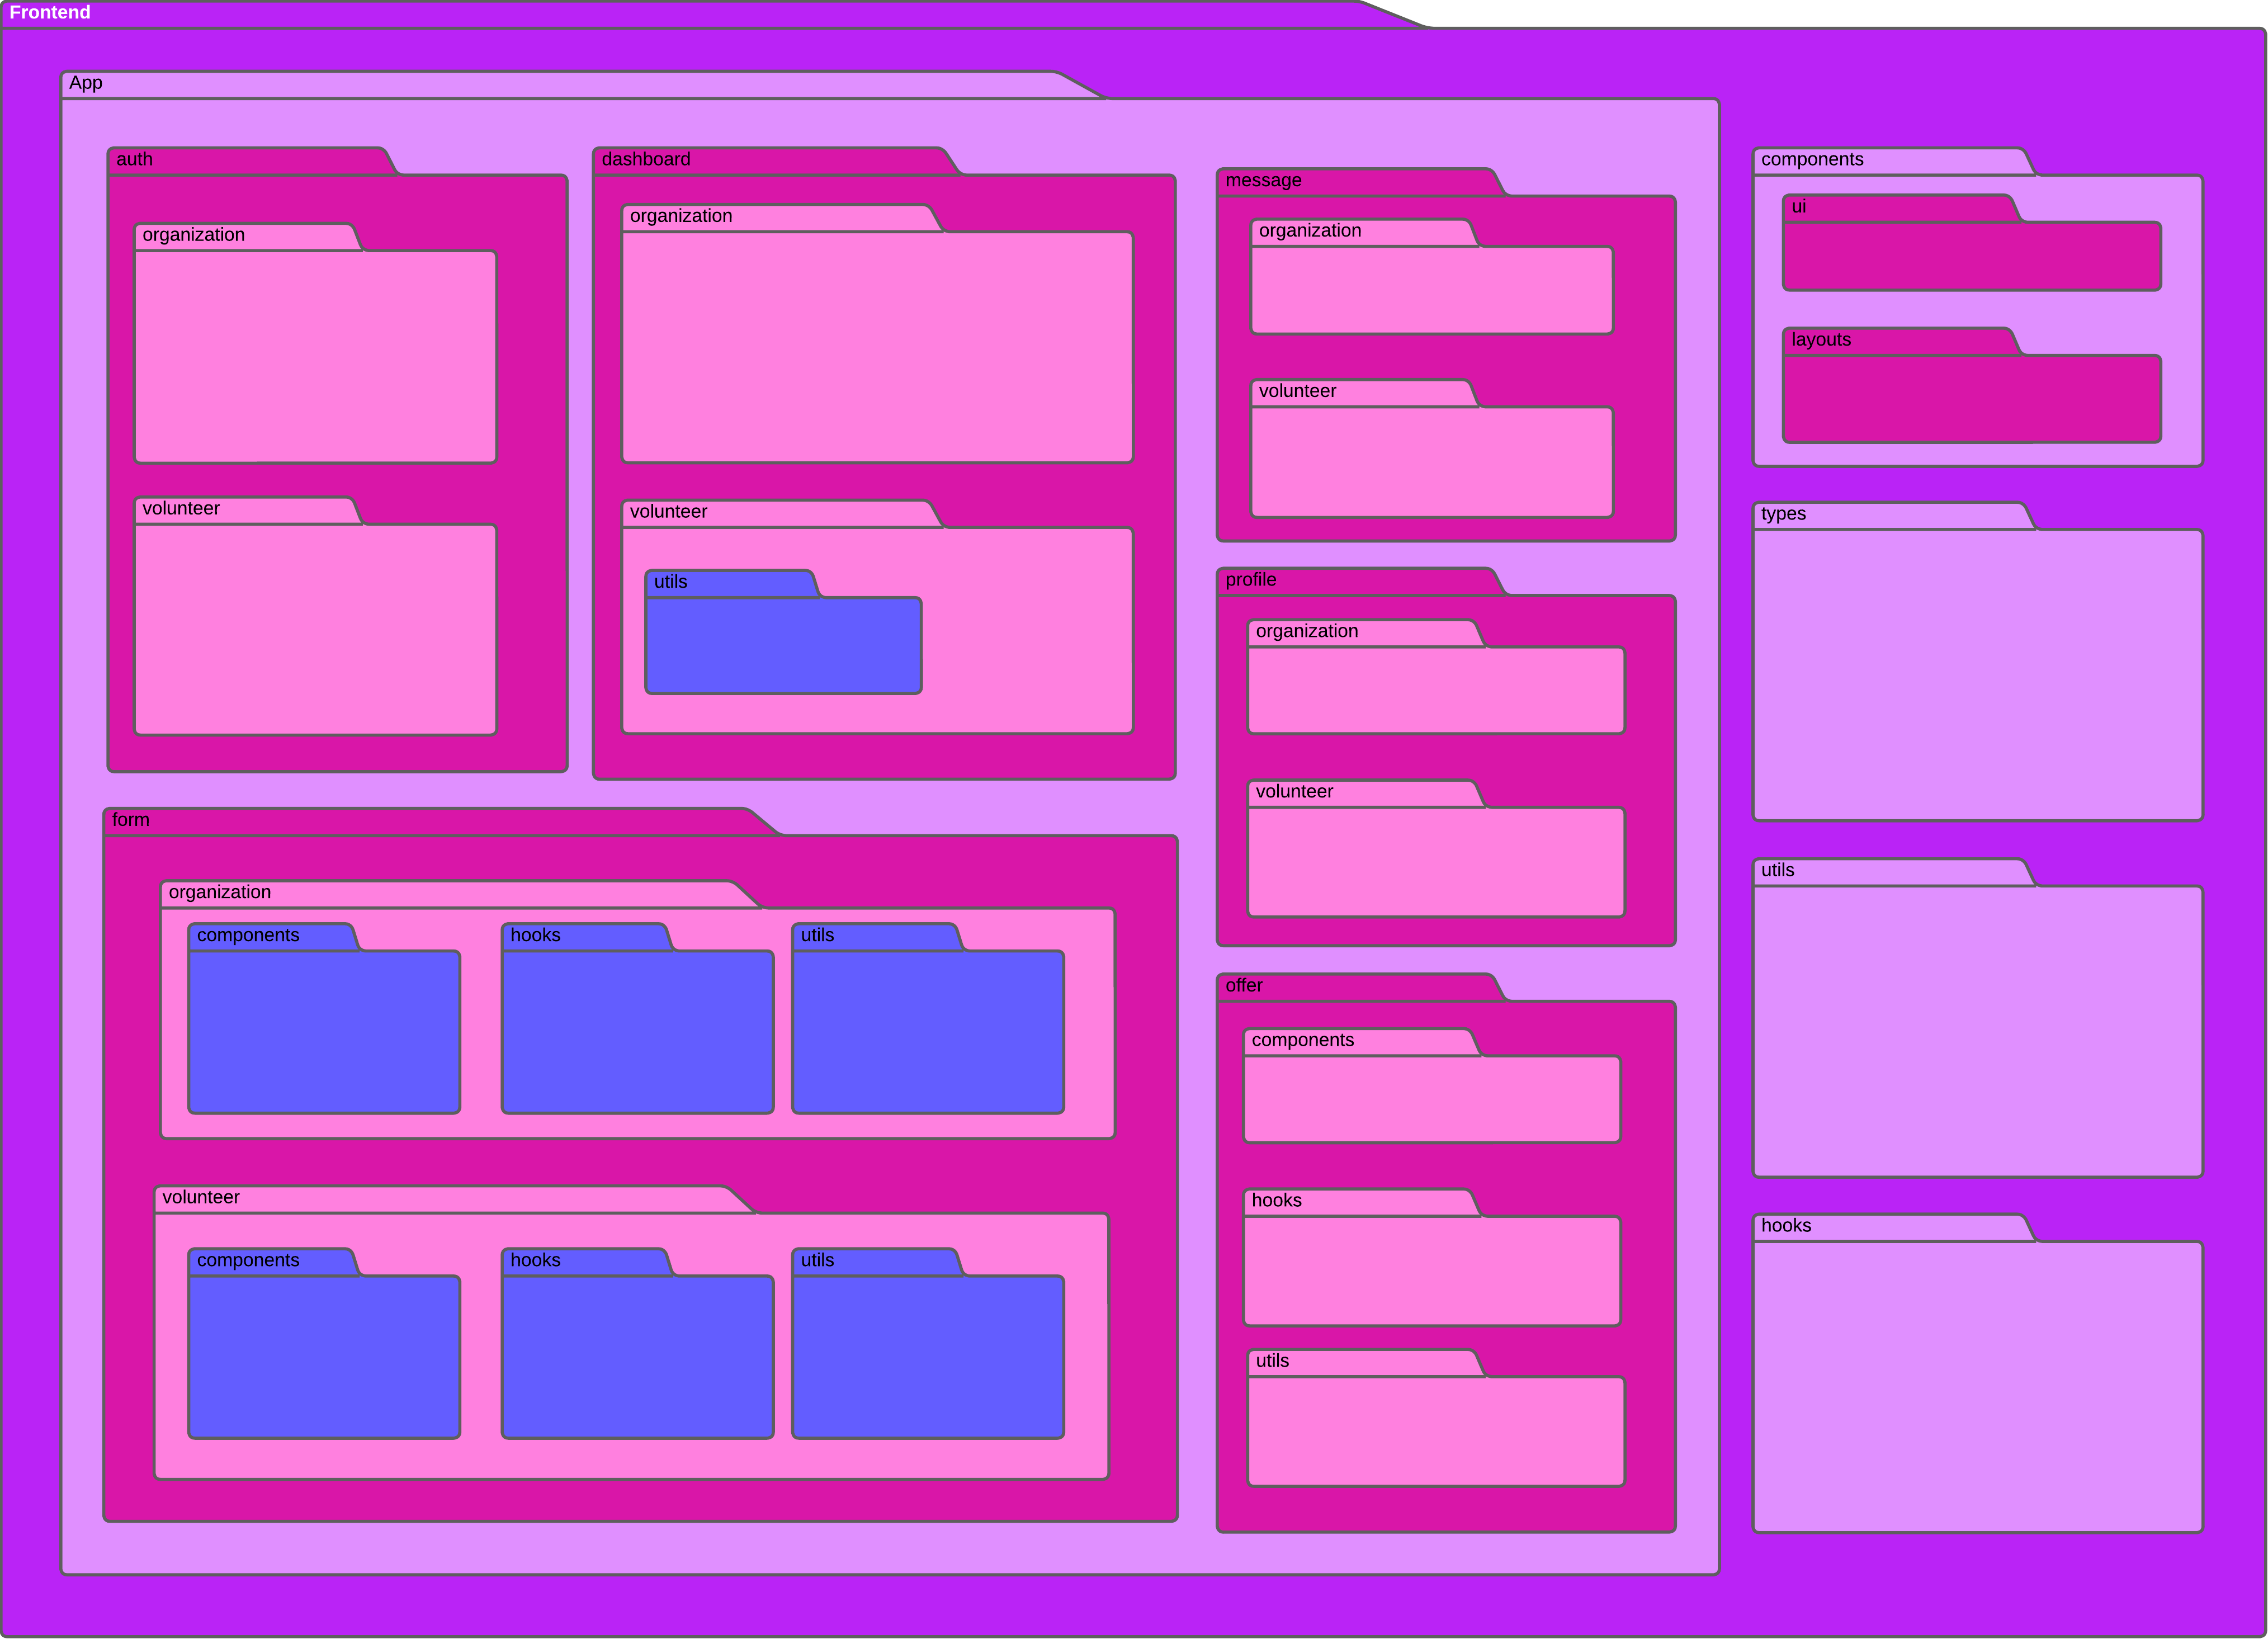
\includegraphics[width=\textwidth, height=\textheight,keepaspectratio]{Immagini/DCSP/Iterazione 1/DCSPFrontend.png}
        \caption{Diagramma delle Classi Software di Progetto}
        \label{fig:diagrammaDCSP2}
\end{figure}

\subsubsection{Diagramma delle Classi Software di Progetto DCSP3: Backend/Controller}
\import{Immagini/DCSP/Iterazione 1/Backend/}{Controller.tex}

\begin{figure}[H]
    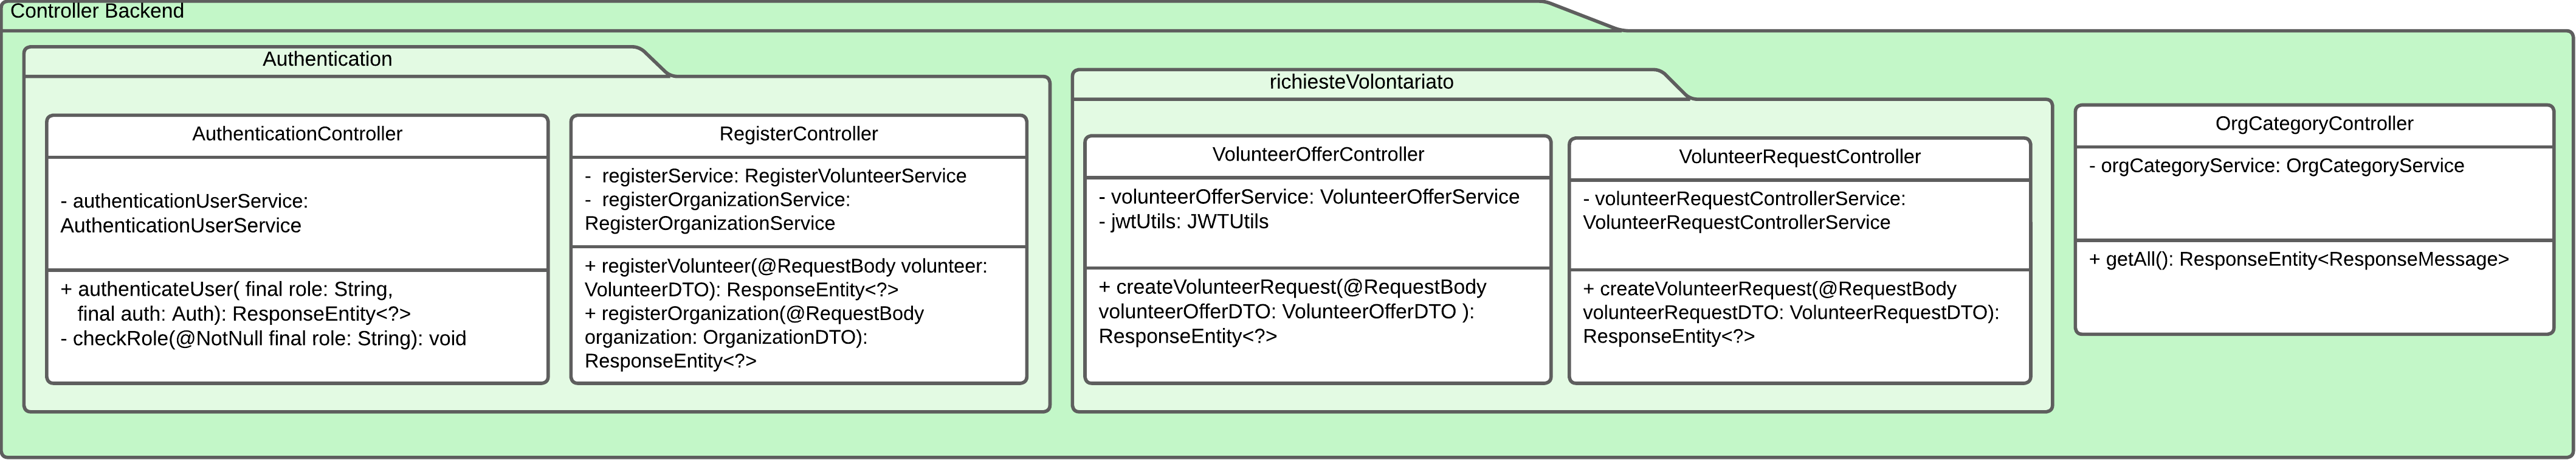
\includegraphics[width=\textwidth, height=\textheight,keepaspectratio]{Immagini/DCSP/Iterazione 1/Backend/DCSPController.png}
        \caption{Diagramma delle Classi Software di Progetto}
        \label{fig:diagrammaDCSP3}
\end{figure}

\subsubsection{Diagramma delle Classi Software di Progetto DCSP4: Backend/Domain}
\import{Immagini/DCSP/Iterazione 1/Backend/}{Domain.tex}

\begin{figure}[H]
    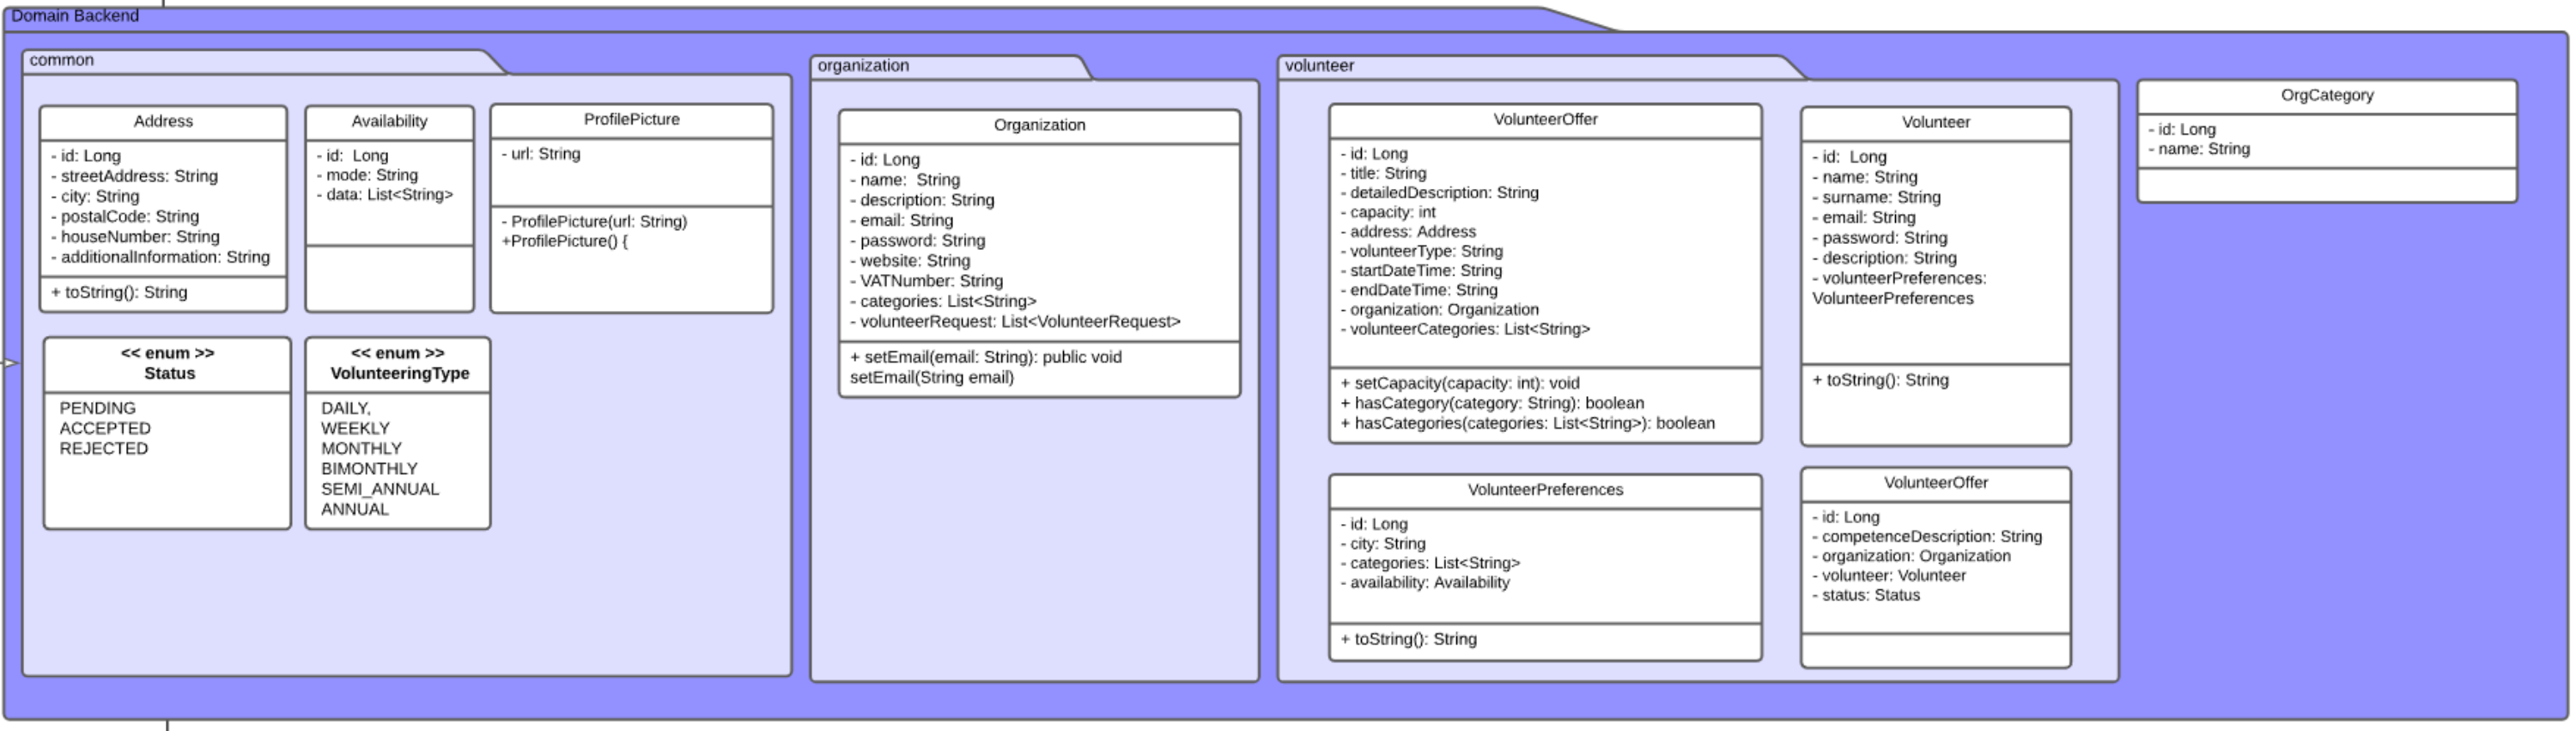
\includegraphics[width=\textwidth, height=\textheight,keepaspectratio]{Immagini/DCSP/Iterazione 1/Backend/DCSPDomain.png}
        \caption{Diagramma delle Classi Software di Progetto}
        \label{fig:diagrammaDCSP4}
\end{figure}

\subsubsection{Diagramma delle Classi Software di Progetto DCSP5: Backend/DTO}
\import{Immagini/DCSP/Iterazione 1/Backend/}{DTO.tex}

\begin{figure}[H]
    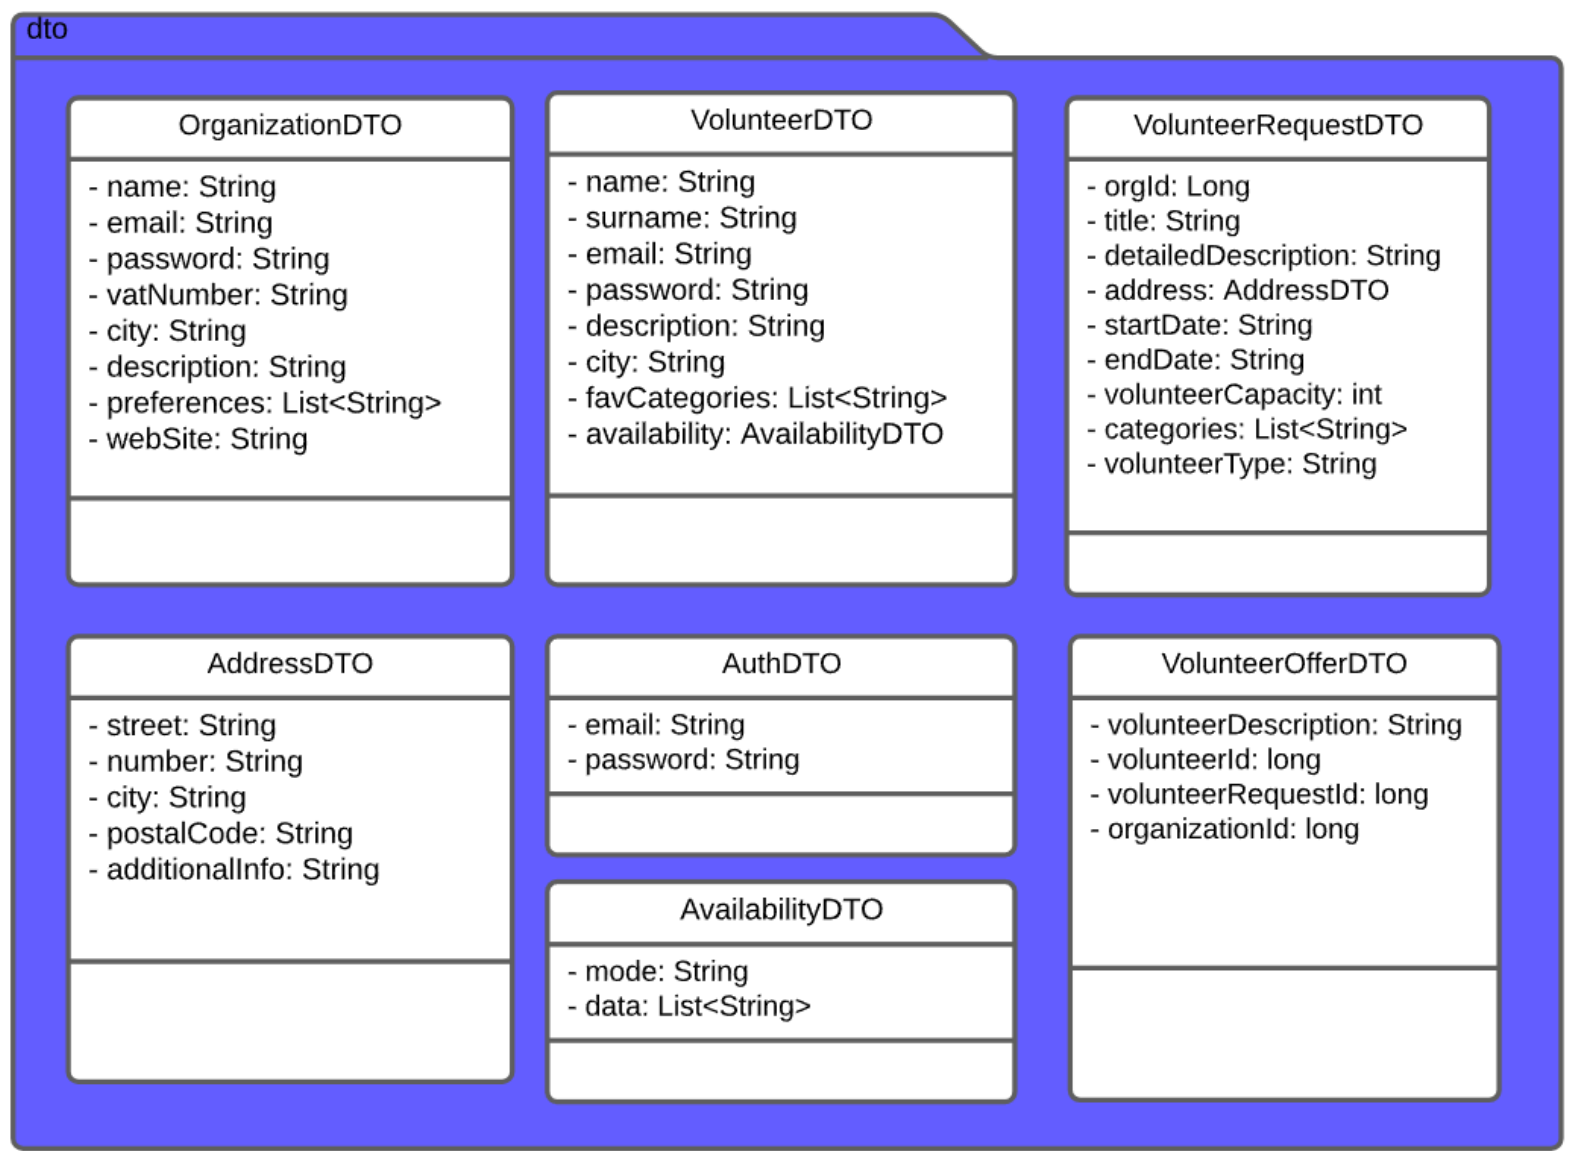
\includegraphics[width=\textwidth, height=\textheight,keepaspectratio]{Immagini/DCSP/Iterazione 1/Backend/DCSPDTO.png}
        \caption{Diagramma delle Classi Software di Progetto}
        \label{fig:diagrammaDCSP5}
\end{figure}

\subsubsection{Diagramma delle Classi Software di Progetto DCSP6: Backend/Mappers}
\import{Immagini/DCSP/Iterazione 1/Backend/}{Mappers.tex}

\begin{figure}[H]
    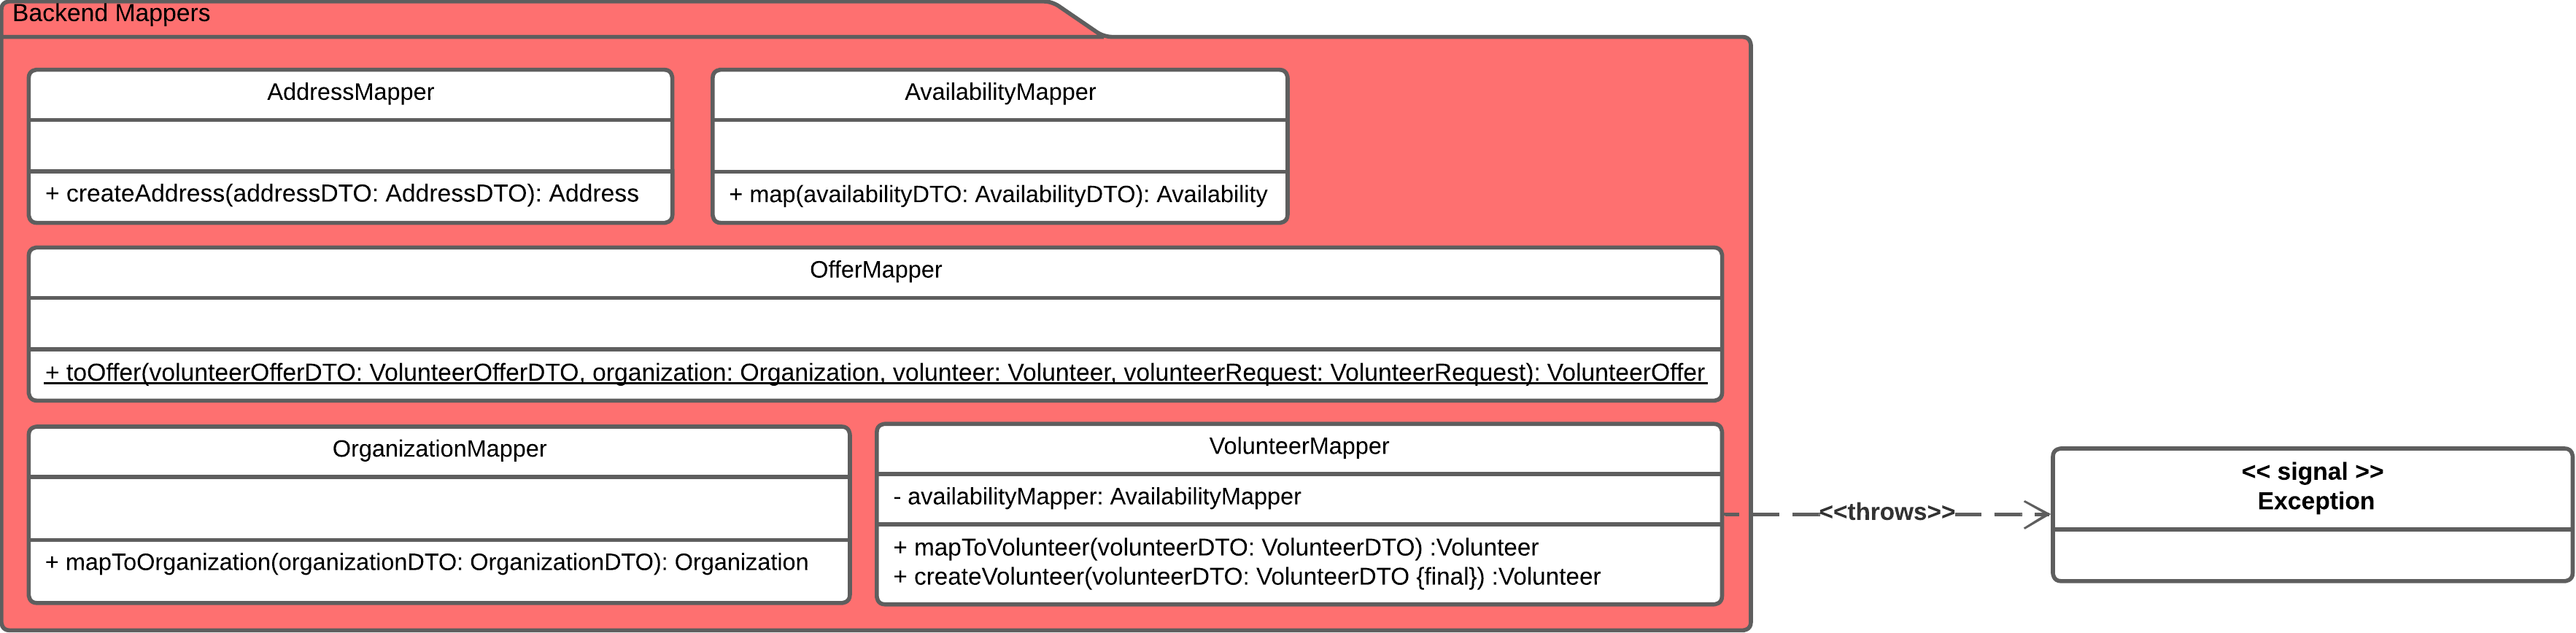
\includegraphics[width=\textwidth, height=\textheight,keepaspectratio]{Immagini/DCSP/Iterazione 1/Backend/DCSPMappers.png}
        \caption{Diagramma delle Classi Software di Progetto}
        \label{fig:diagrammaDCSP6}
\end{figure}

\subsubsection{Diagramma delle Classi Software di Progetto DCSP7: Backend/Service}
\import{Immagini/DCSP/Iterazione 1/Backend/}{Service.tex}

\begin{figure}[H]
    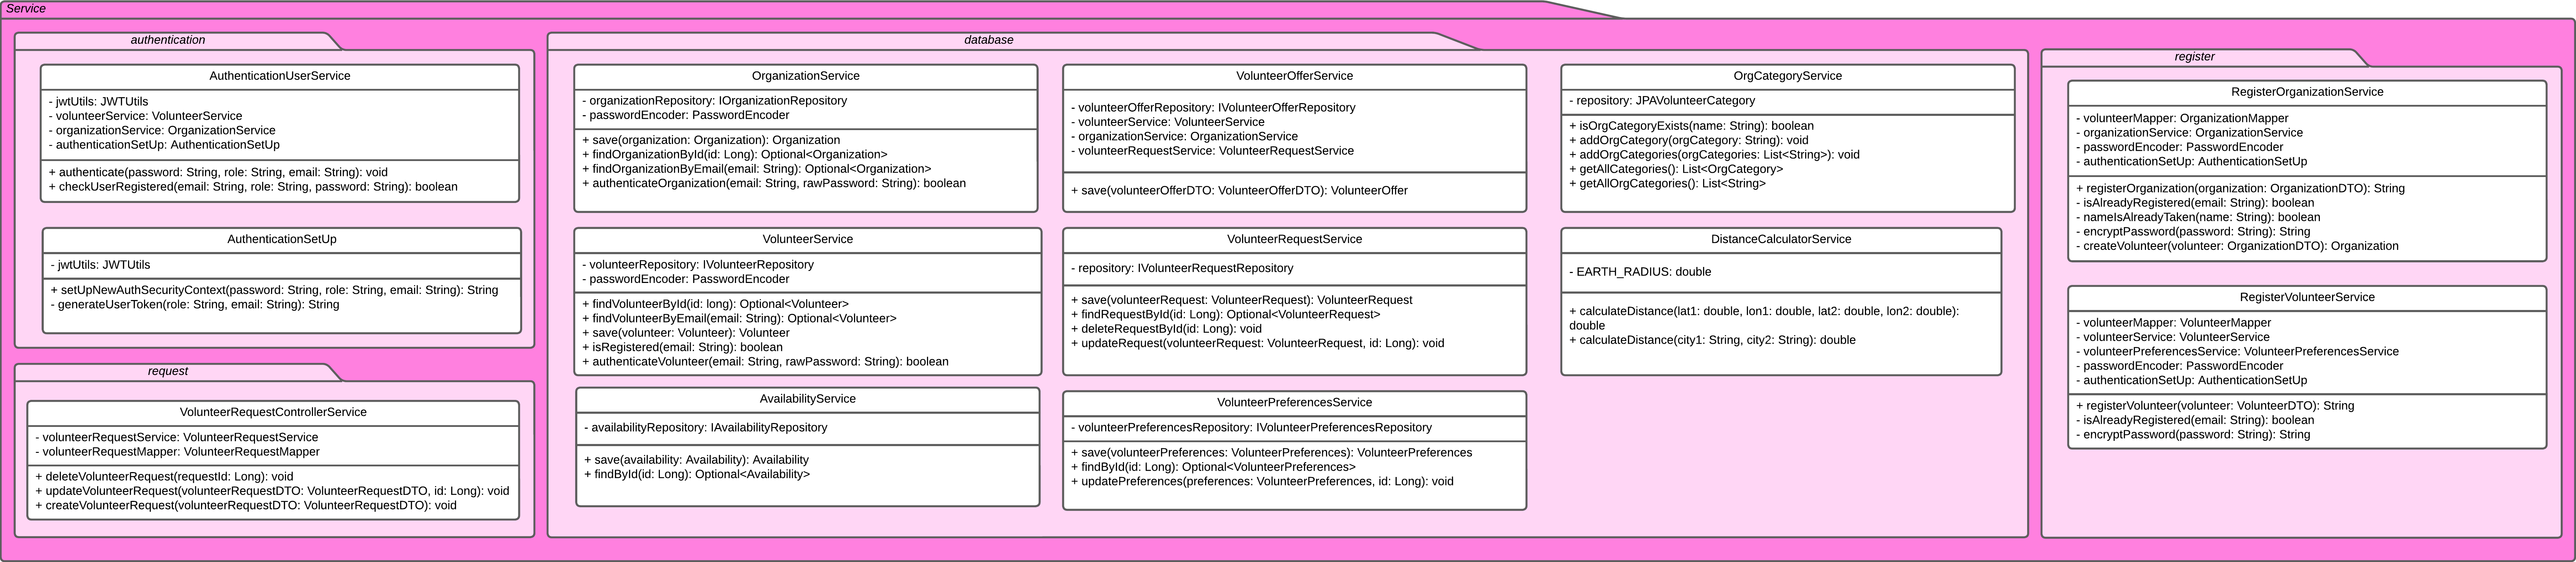
\includegraphics[width=\textwidth, height=\textheight,keepaspectratio]{Immagini/DCSP/Iterazione 1/Backend/DCSPService.png}
        \caption{Diagramma delle Classi Software di Progetto}
        \label{fig:diagrammaDCSP7}
\end{figure}

\subsubsection{Diagramma delle Classi Software di Progetto DCSP8: Backend/Repository}
\import{Immagini/DCSP/Iterazione 1/Backend/}{Repository.tex}

\begin{figure}[H]
    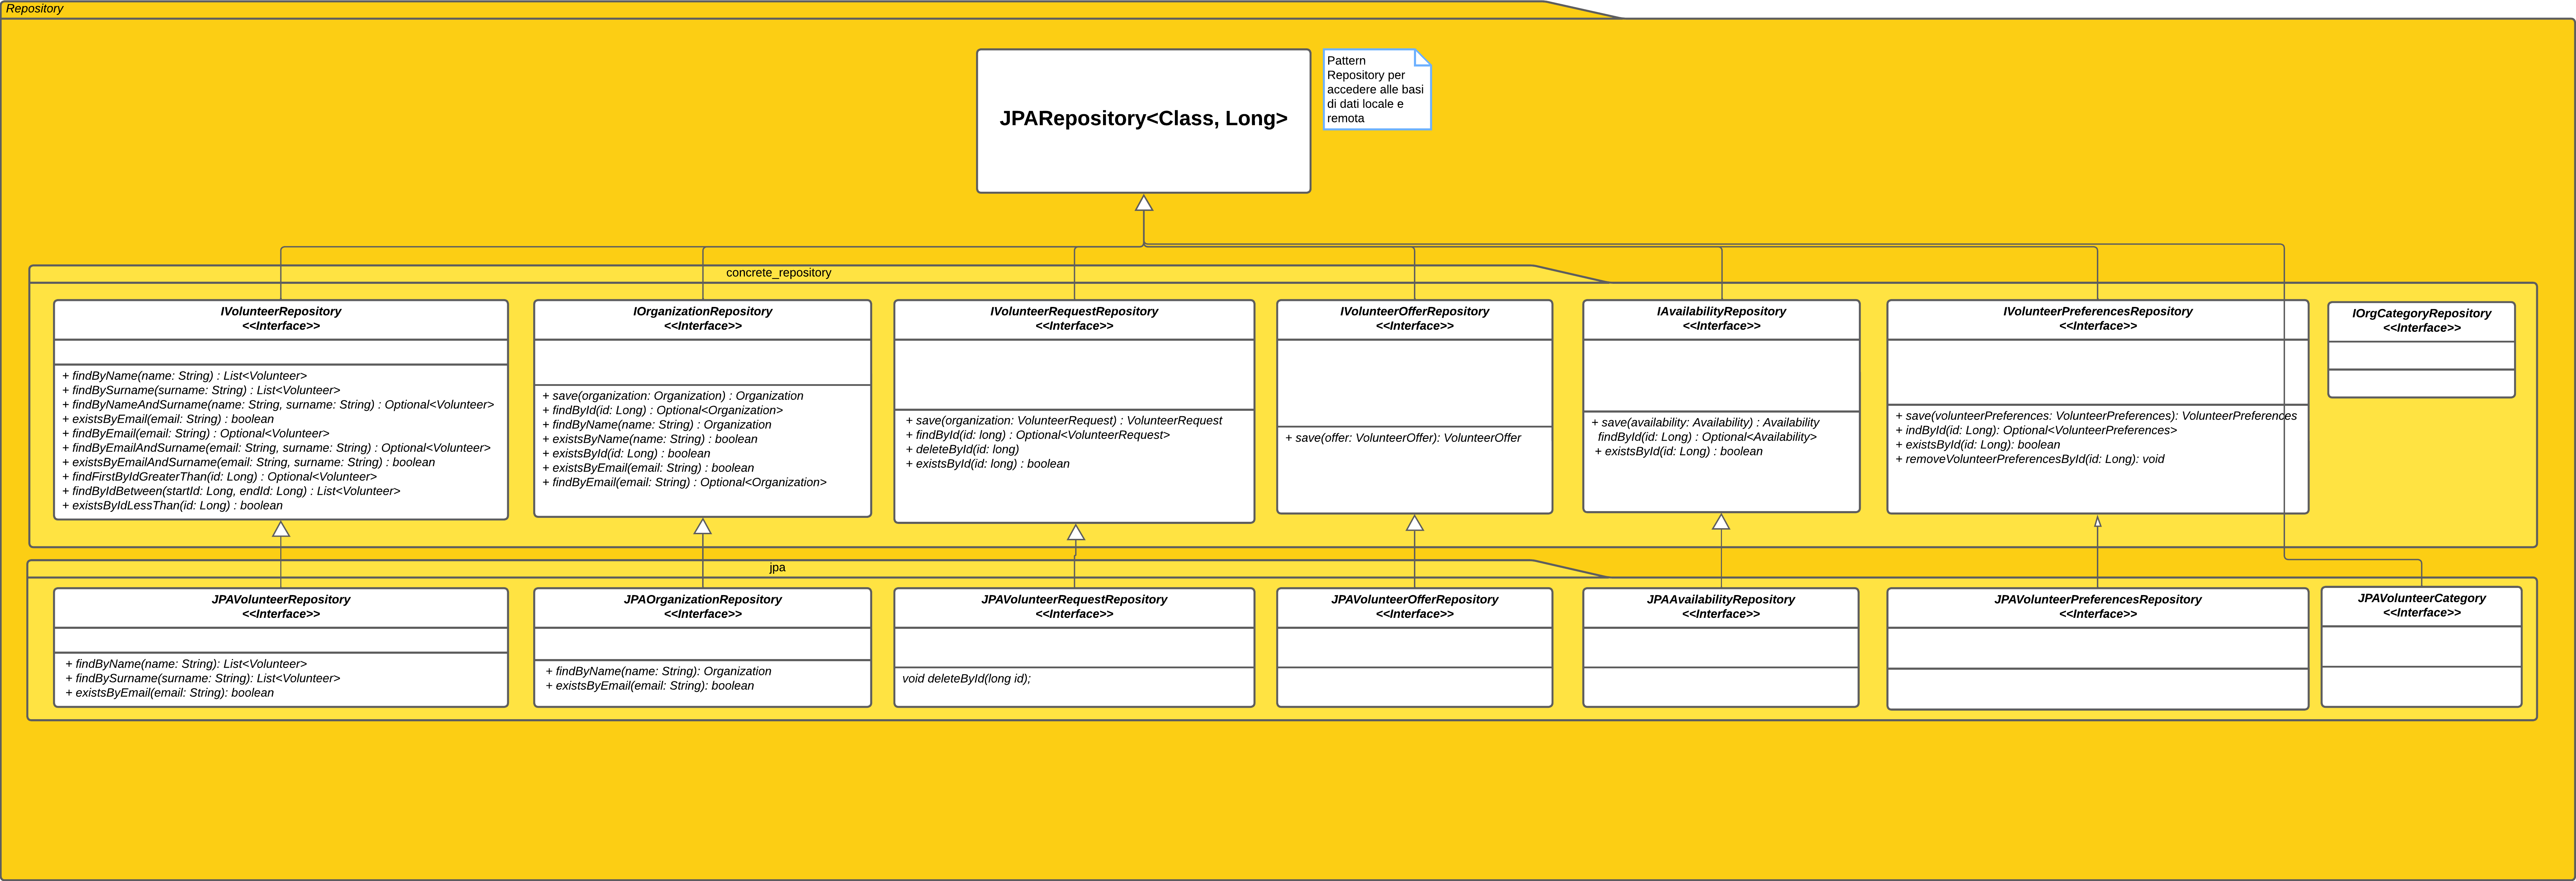
\includegraphics[width=\textwidth, height=\textheight,keepaspectratio]{Immagini/DCSP/Iterazione 1/Backend/DCSPRepository.png}
        \caption{Diagramma delle Classi Software di Progetto}
        \label{fig:diagrammaDCSP8}
\end{figure}

\subsection{Diagramma dell'Architettura Logica}

\subsubsection{Diagramma dell'Architettura Logica}
\import{Immagini/AL/Iterazione 1}{ArchitetturaLogica.tex}

\begin{figure}[H]
    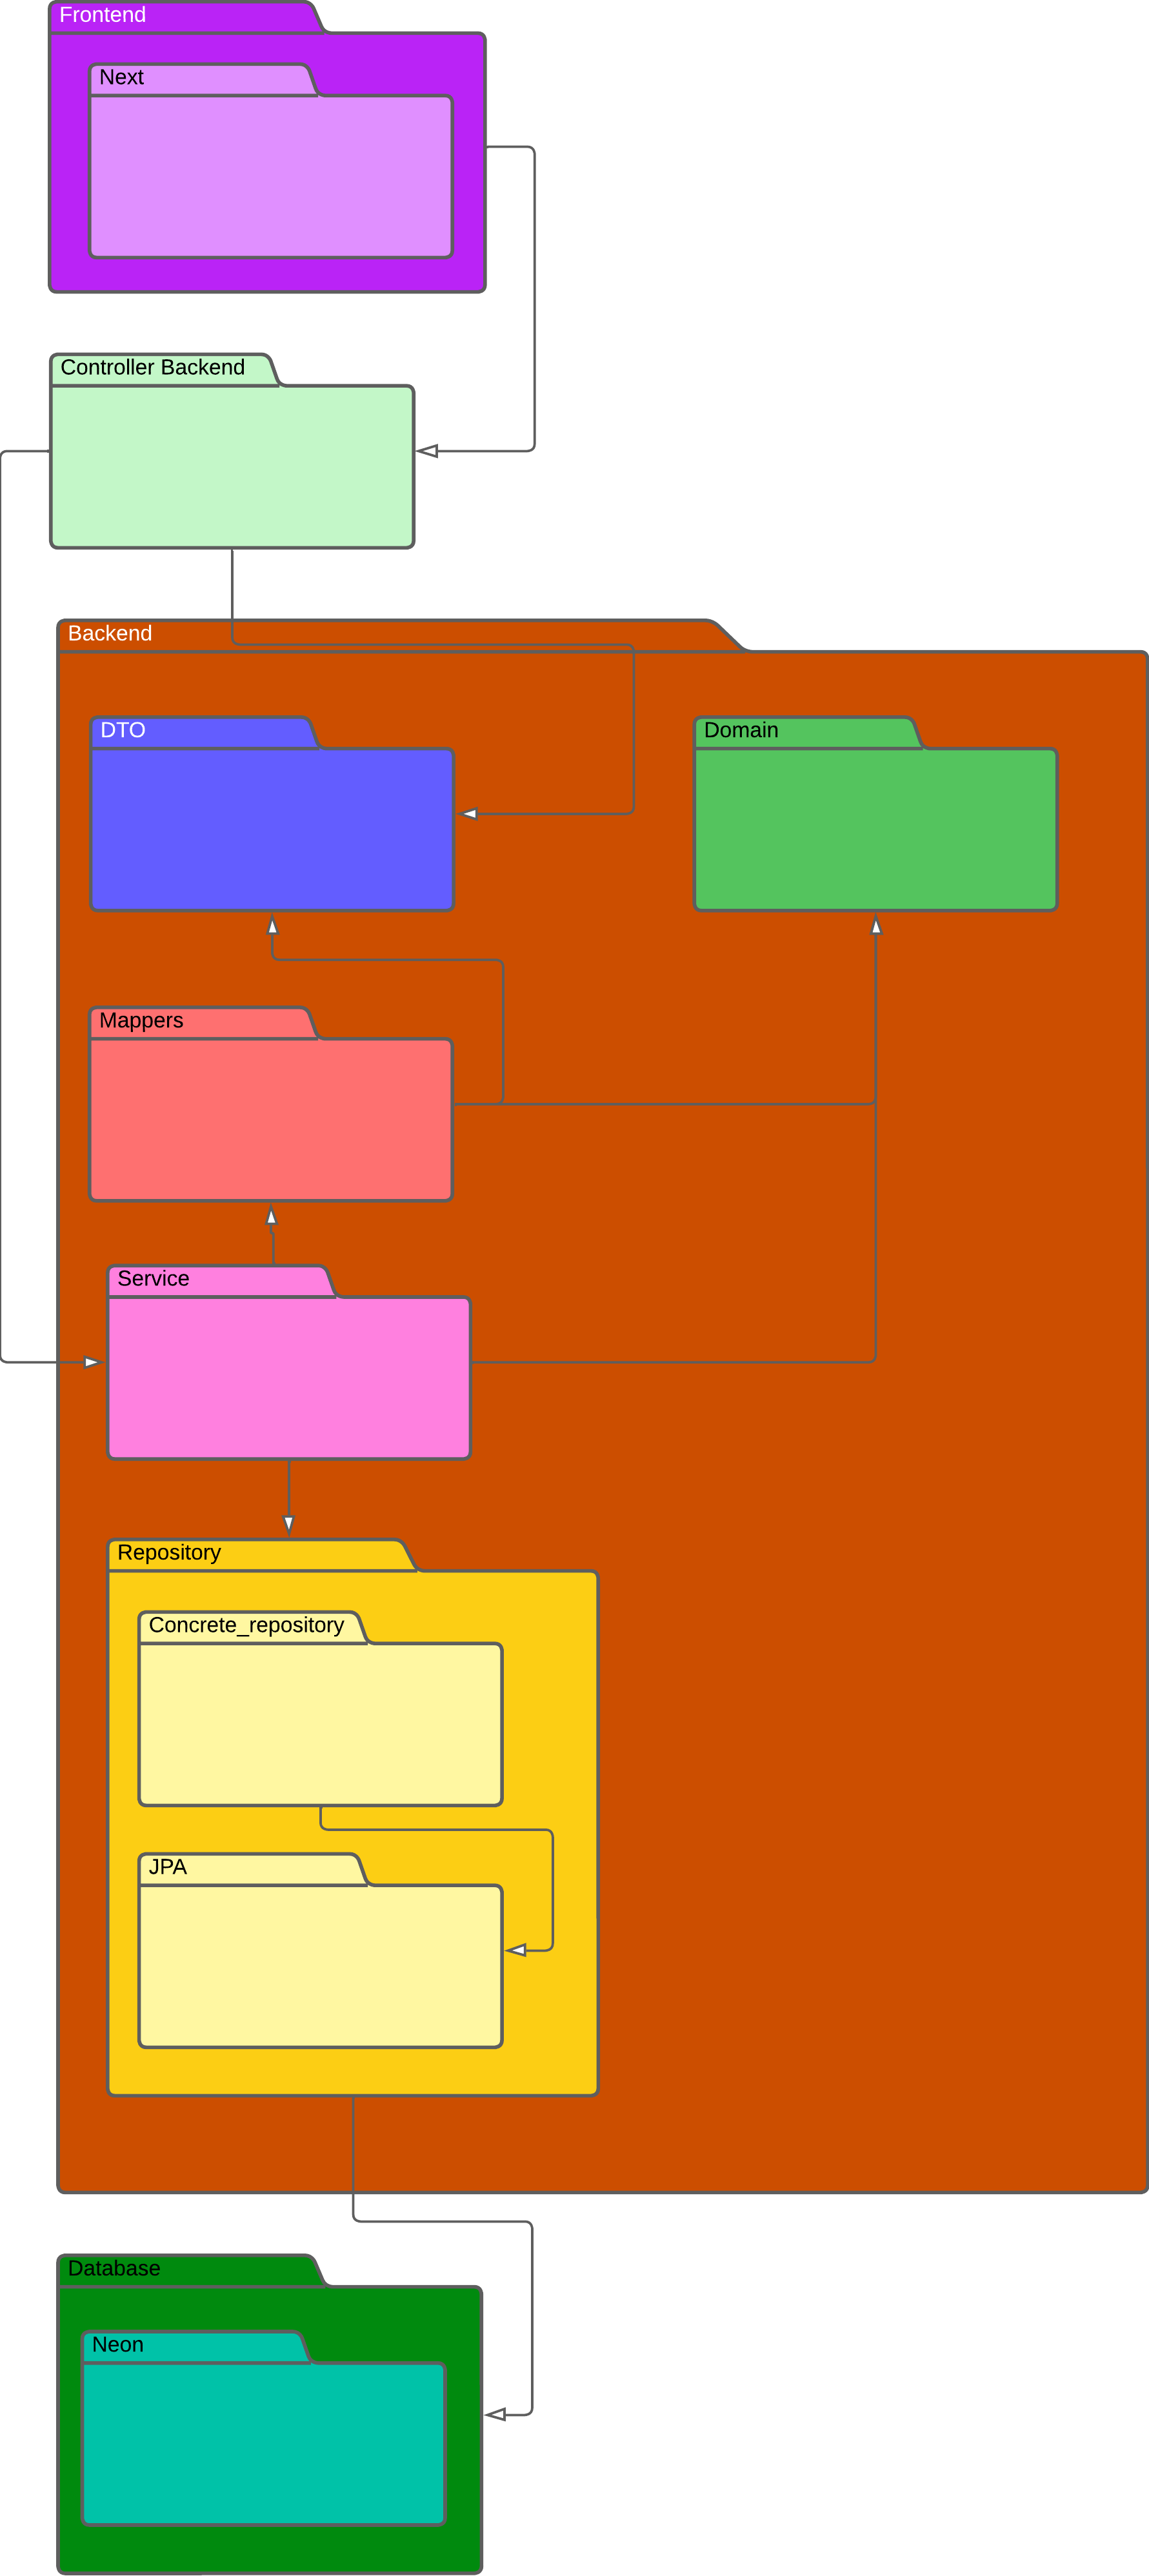
\includegraphics[width=\textwidth, height=\textheight,keepaspectratio]{Immagini/AL/Iterazione 1/ALArchitetturaLogica.png}
        \caption{Diagramma dell'Architettura Logica}
        \label{fig:diagrammaAL1}
\end{figure}

\subsection{Pattern}
\import{Pattern/Iterazione 1/}{Introduzione.tex}


\subsubsection{Design Patterns}
\import{Pattern/Iterazione 1/}{Design Patterns.tex}

\section*{\Huge \textbf{Iterazione 2}}
\addcontentsline{toc}{section}{Iterazione 2}
\setcounter{section}{0} 
\renewcommand{\thesubsection}{\arabic{subsection}} 

\section{Diagramma di Gantt}
Questi sono i diagrammi di Gantt per l'iterazione 2.

\begin{figure}[H]
    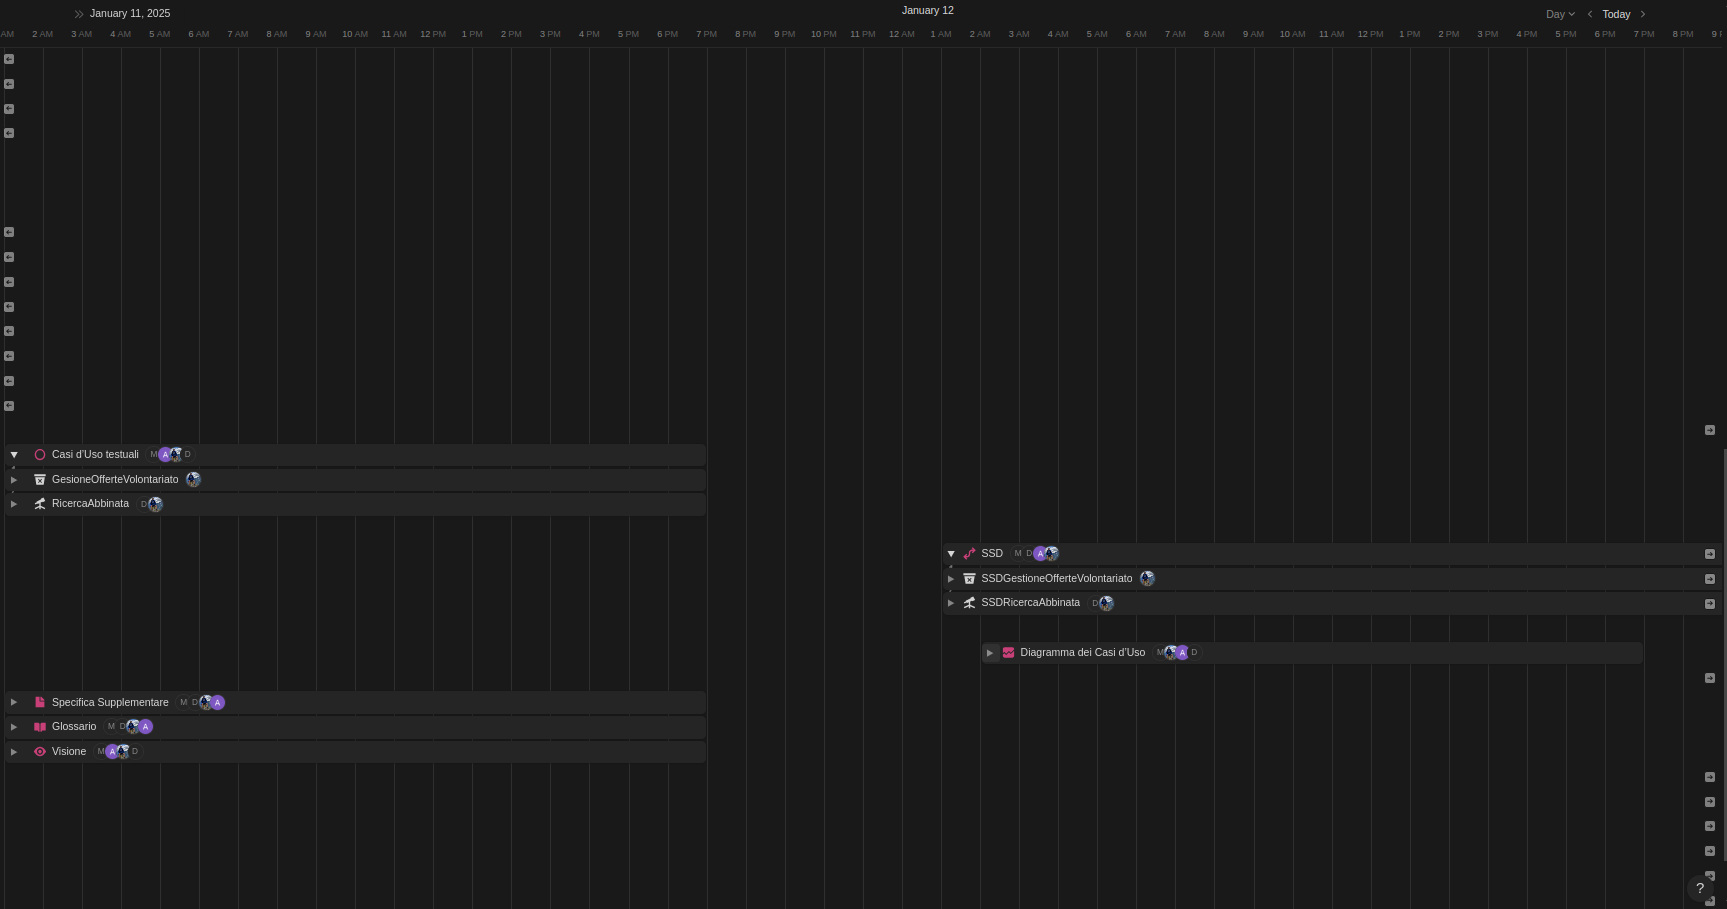
\includegraphics[width=\textwidth,keepaspectratio]{Immagini/Gantt/Iterazione 2/Gantt12.png}
        \caption{Diagramma di Gantt 12} 
        \label{fig:Gantt12}
\end{figure}

\begin{figure}[H]
    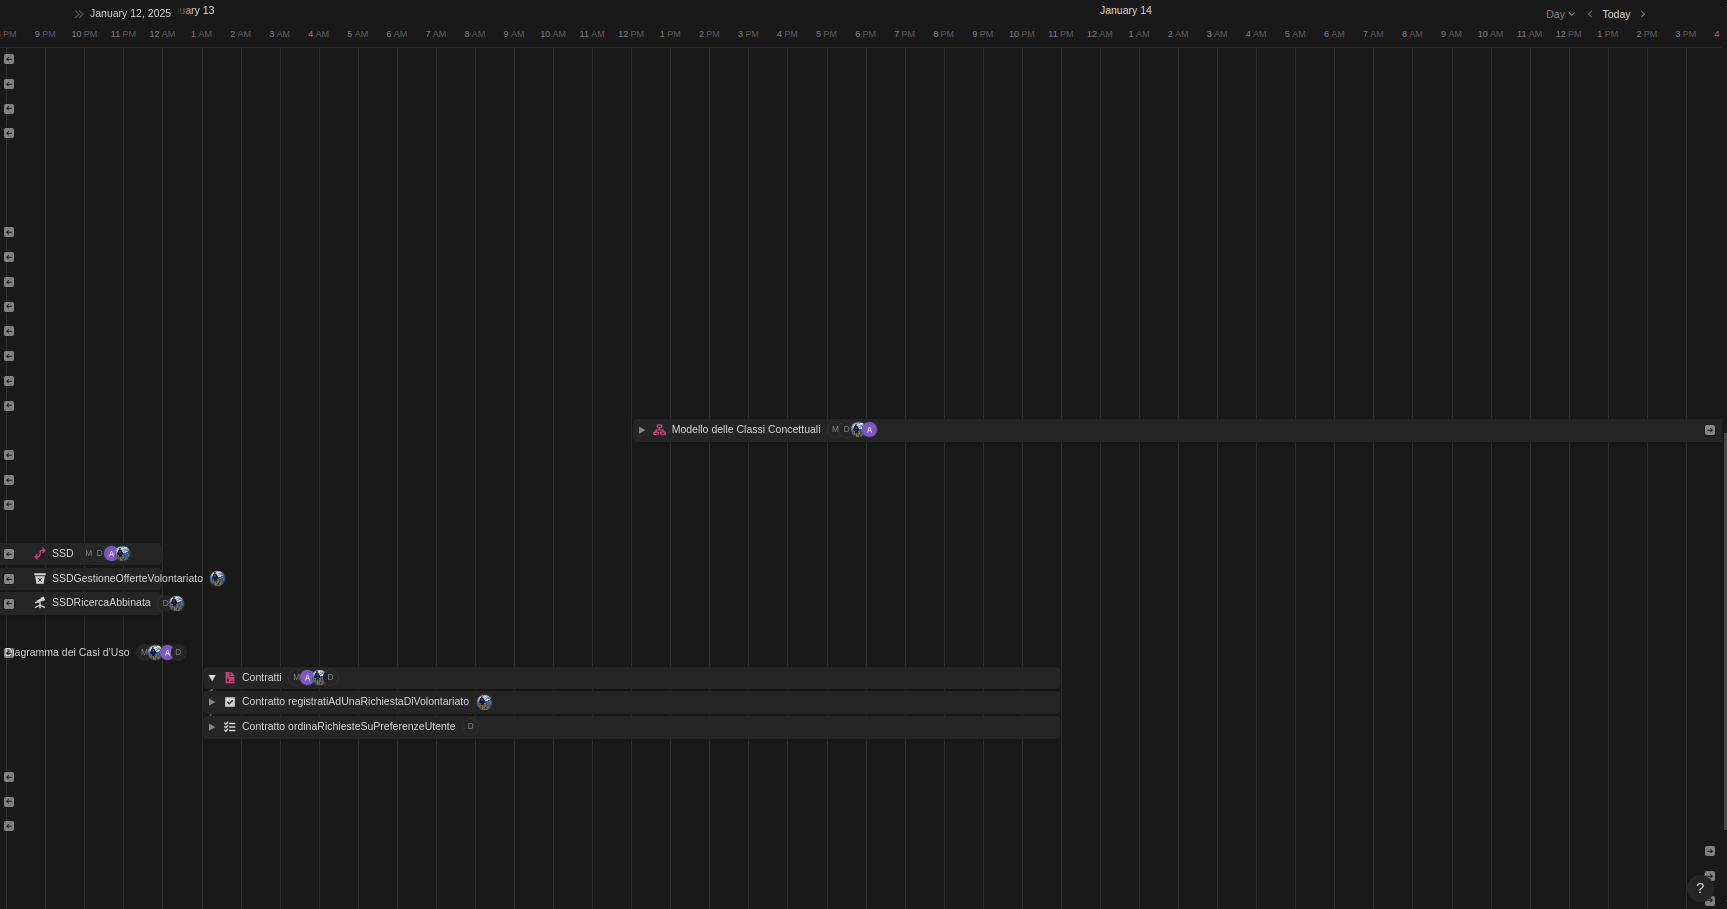
\includegraphics[width=\textwidth,keepaspectratio]{Immagini/Gantt/Iterazione 2/Gantt13.png}
        \caption{Diagramma di Gantt 13} 
        \label{fig:Gantt13}
\end{figure}

\begin{figure}[H]
    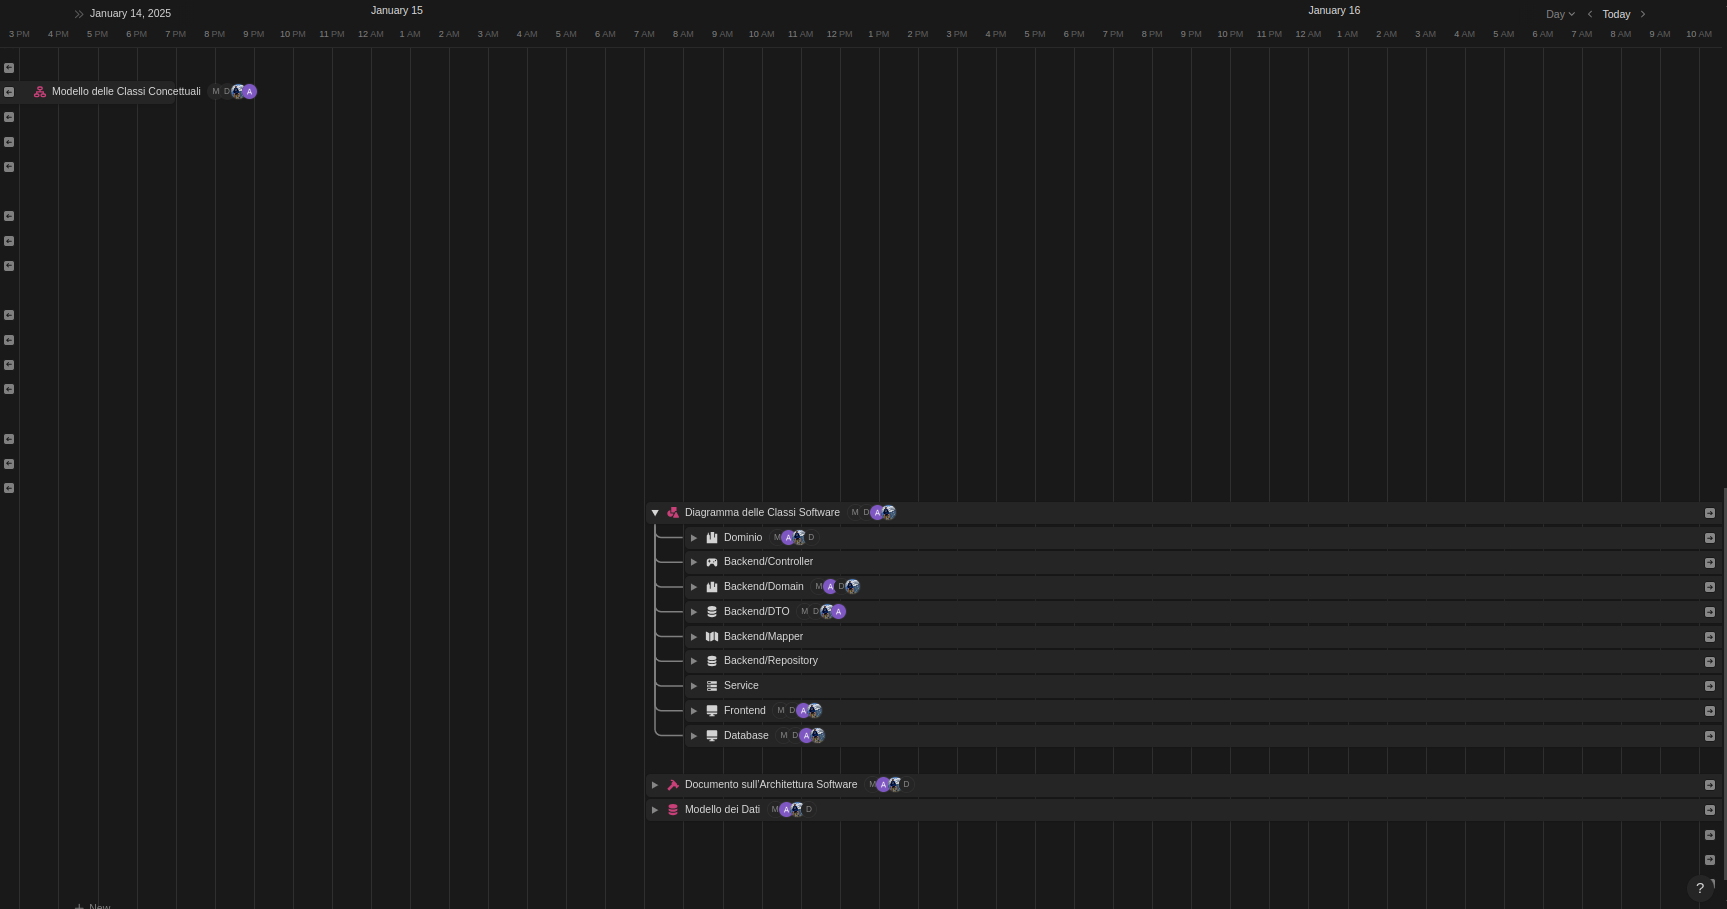
\includegraphics[width=\textwidth,keepaspectratio]{Immagini/Gantt/Iterazione 2/Gantt14.png}
        \caption{Diagramma di Gantt 13} 
        \label{fig:Gantt13}
\end{figure}

\begin{figure}[H]
    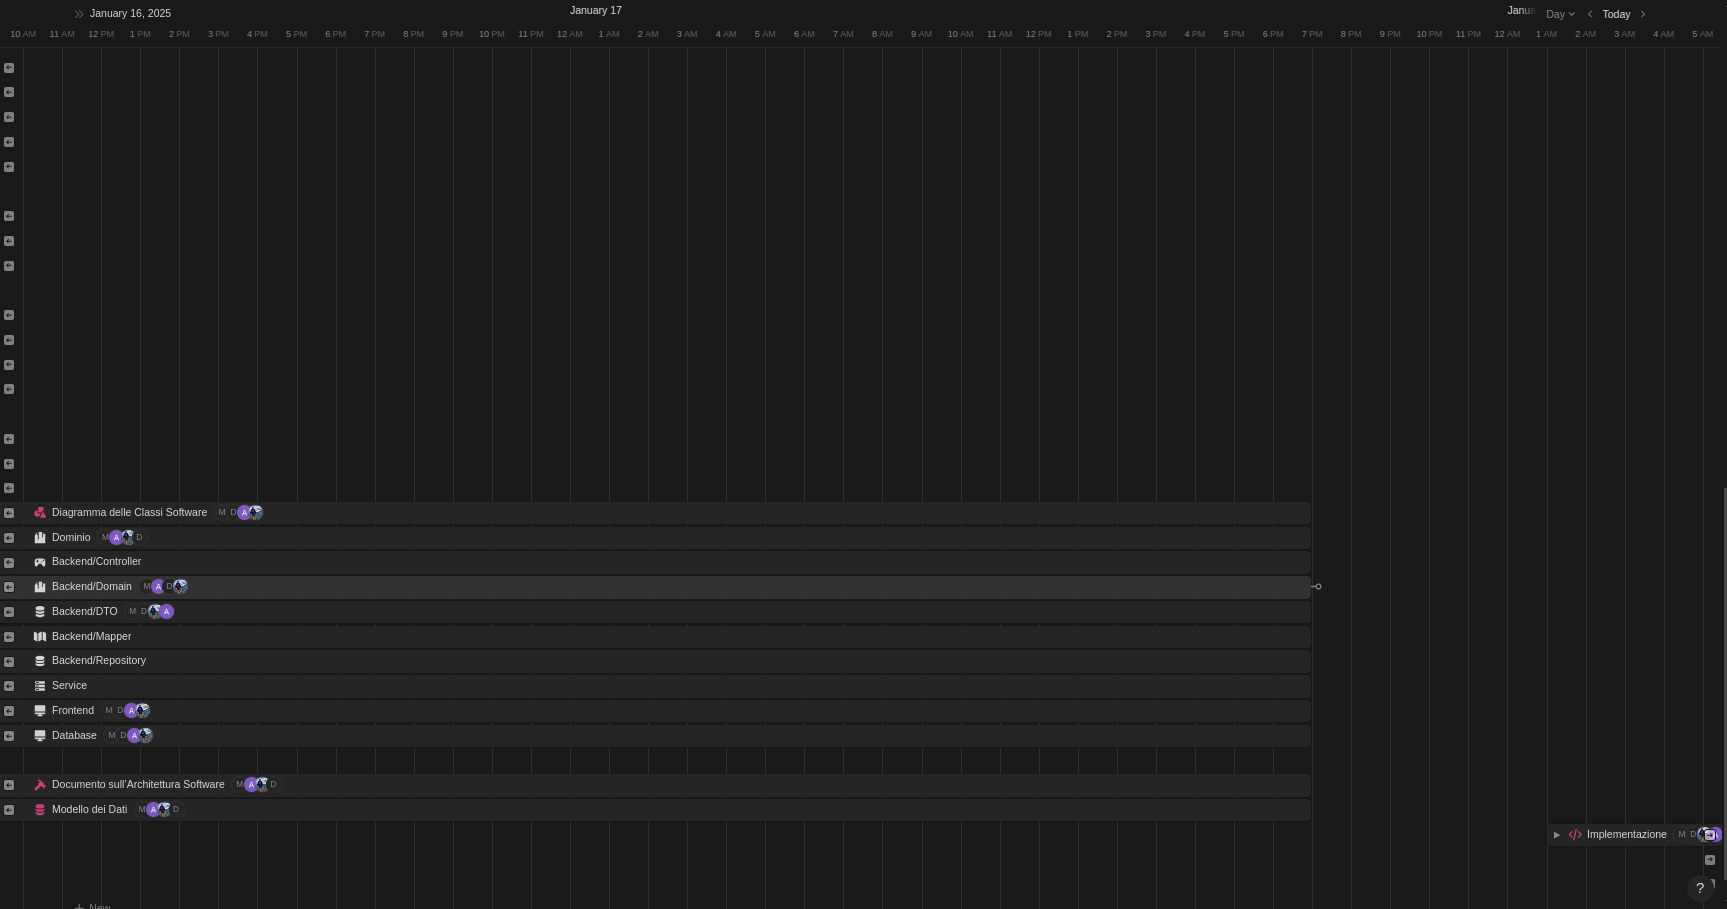
\includegraphics[width=\textwidth,keepaspectratio]{Immagini/Gantt/Iterazione 2/Gantt15.png}
        \caption{Diagramma di Gantt 15} 
        \label{fig:Gantt15}
\end{figure}

\begin{figure}[H]
    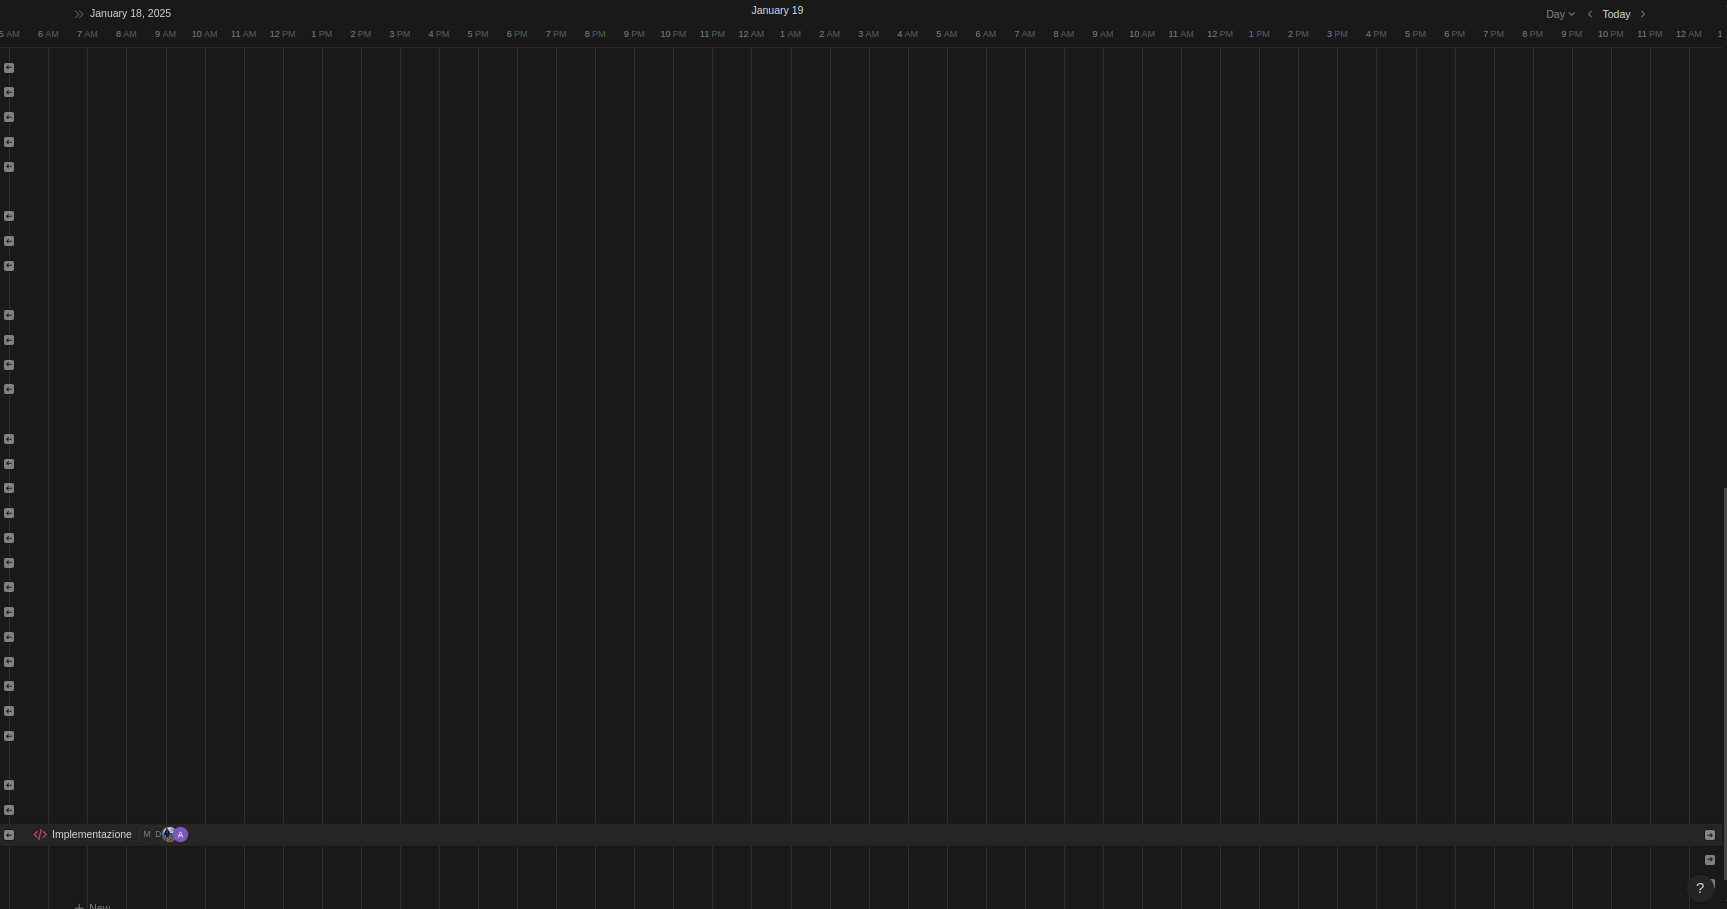
\includegraphics[width=\textwidth,keepaspectratio]{Immagini/Gantt/Iterazione 2/Gantt16.png}
        \caption{Diagramma di Gantt 16} 
        \label{fig:Gantt16}
\end{figure}

\begin{figure}[H]
    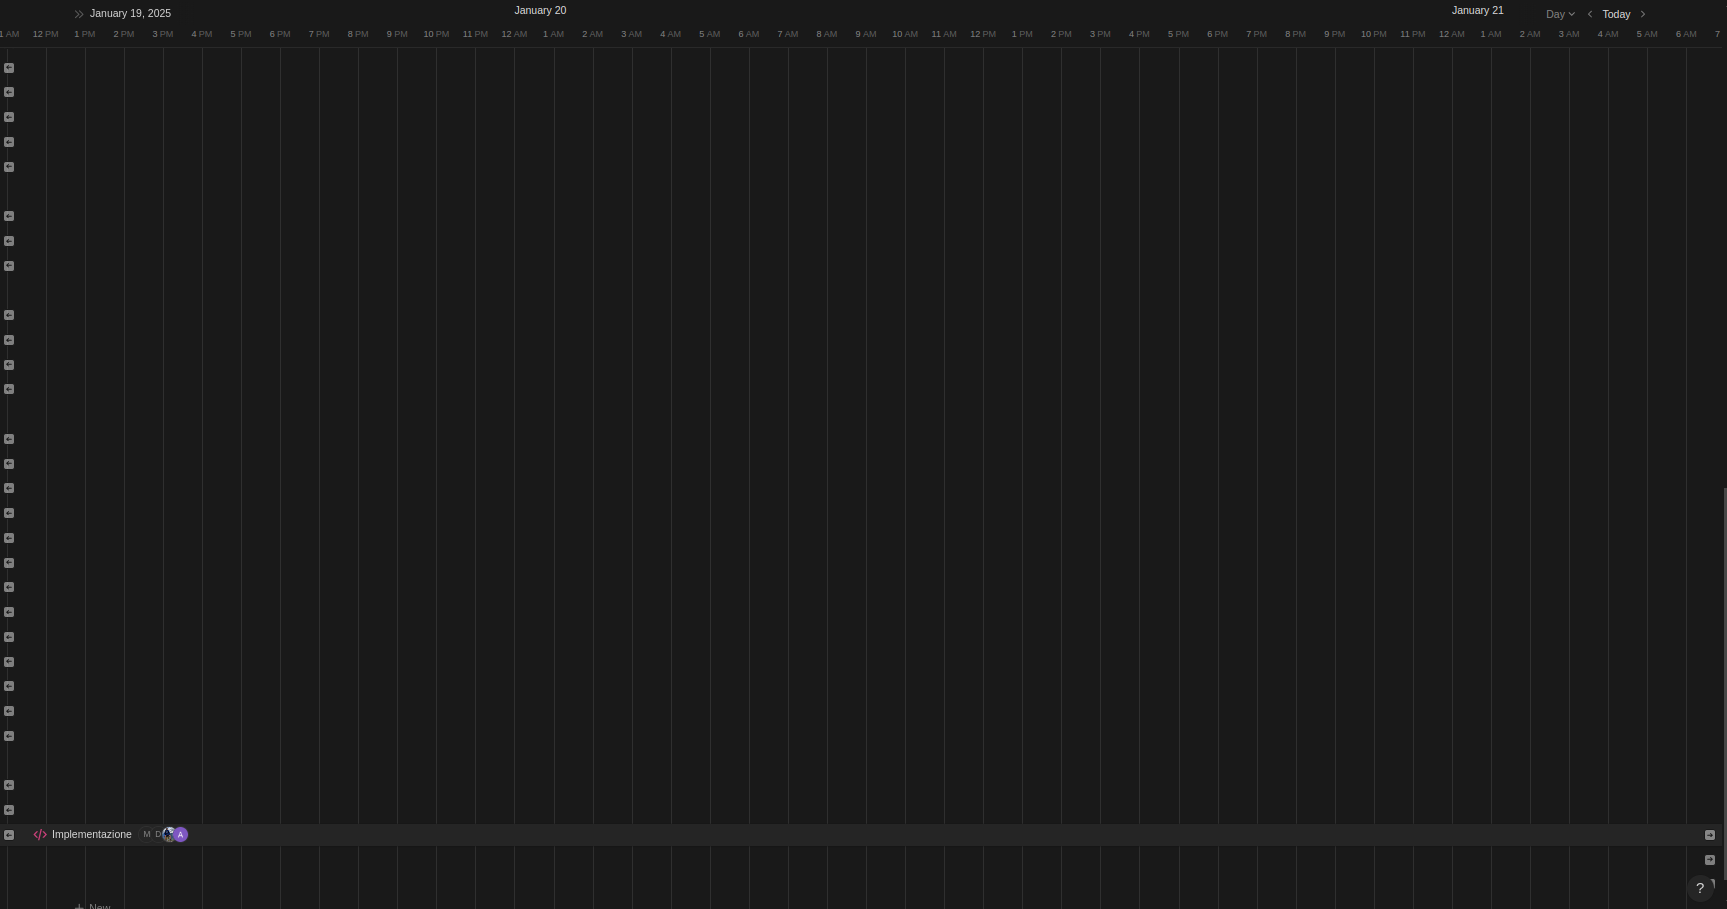
\includegraphics[width=\textwidth,keepaspectratio]{Immagini/Gantt/Iterazione 2/Gantt17.png}
        \caption{Diagramma di Gantt 17} 
        \label{fig:Gantt17}
\end{figure}

\begin{figure}[H]
    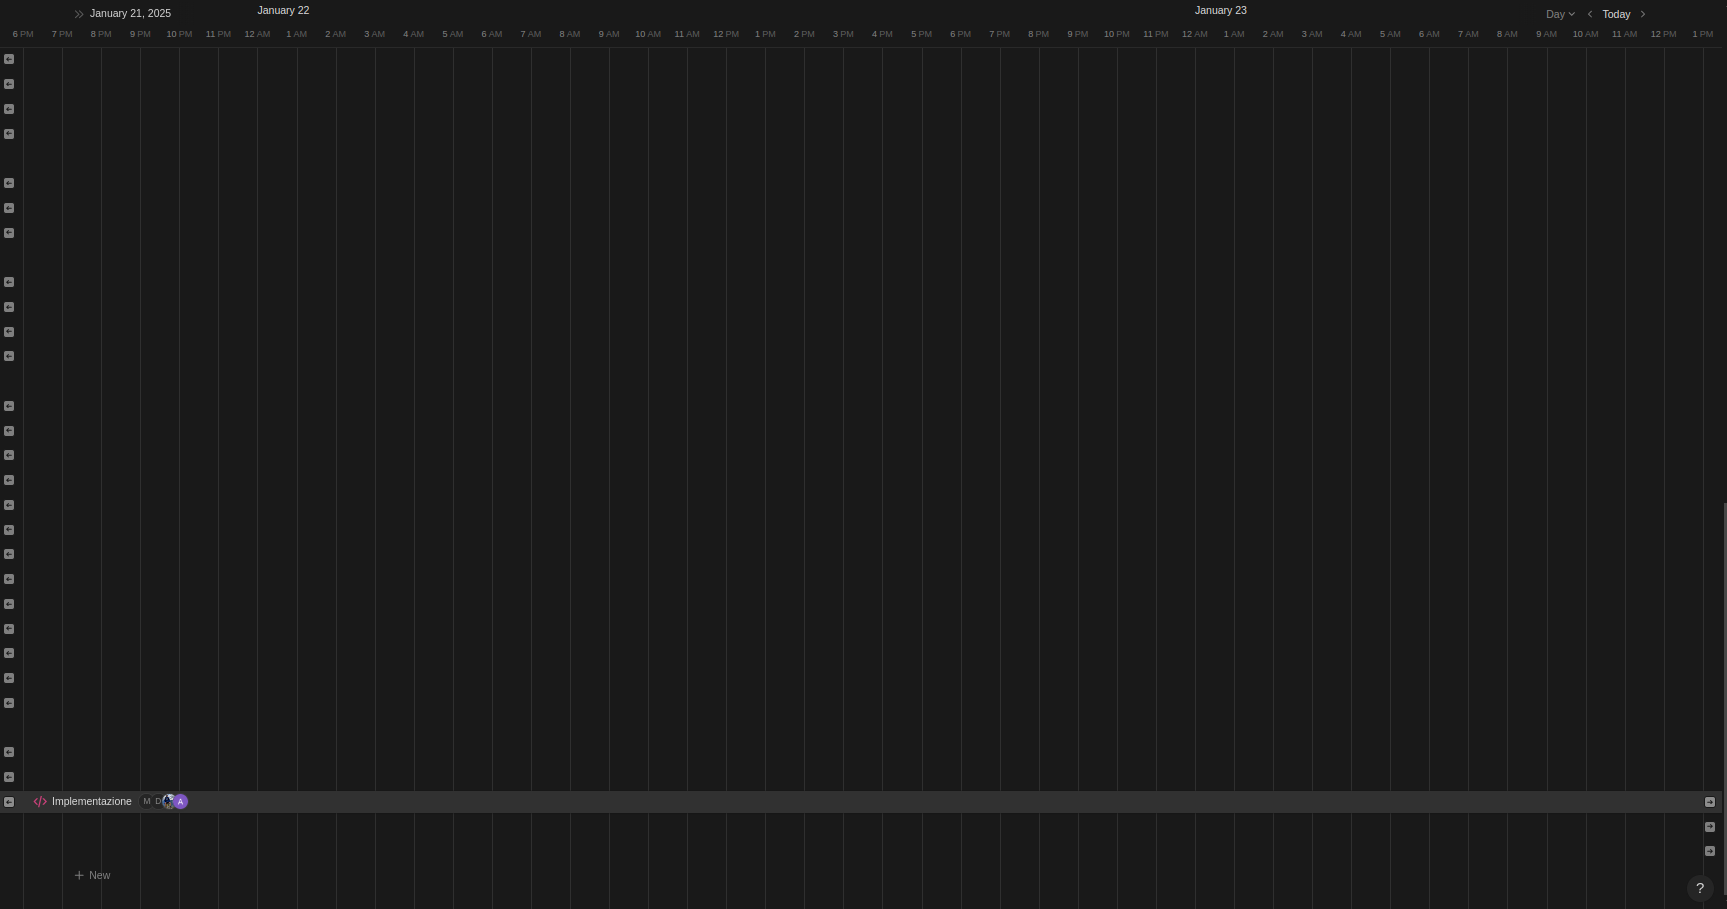
\includegraphics[width=\textwidth,keepaspectratio]{Immagini/Gantt/Iterazione 2/Gantt18.png}
        \caption{Diagramma di Gantt 18} 
        \label{fig:Gantt18}
\end{figure}

\begin{figure}[H]
    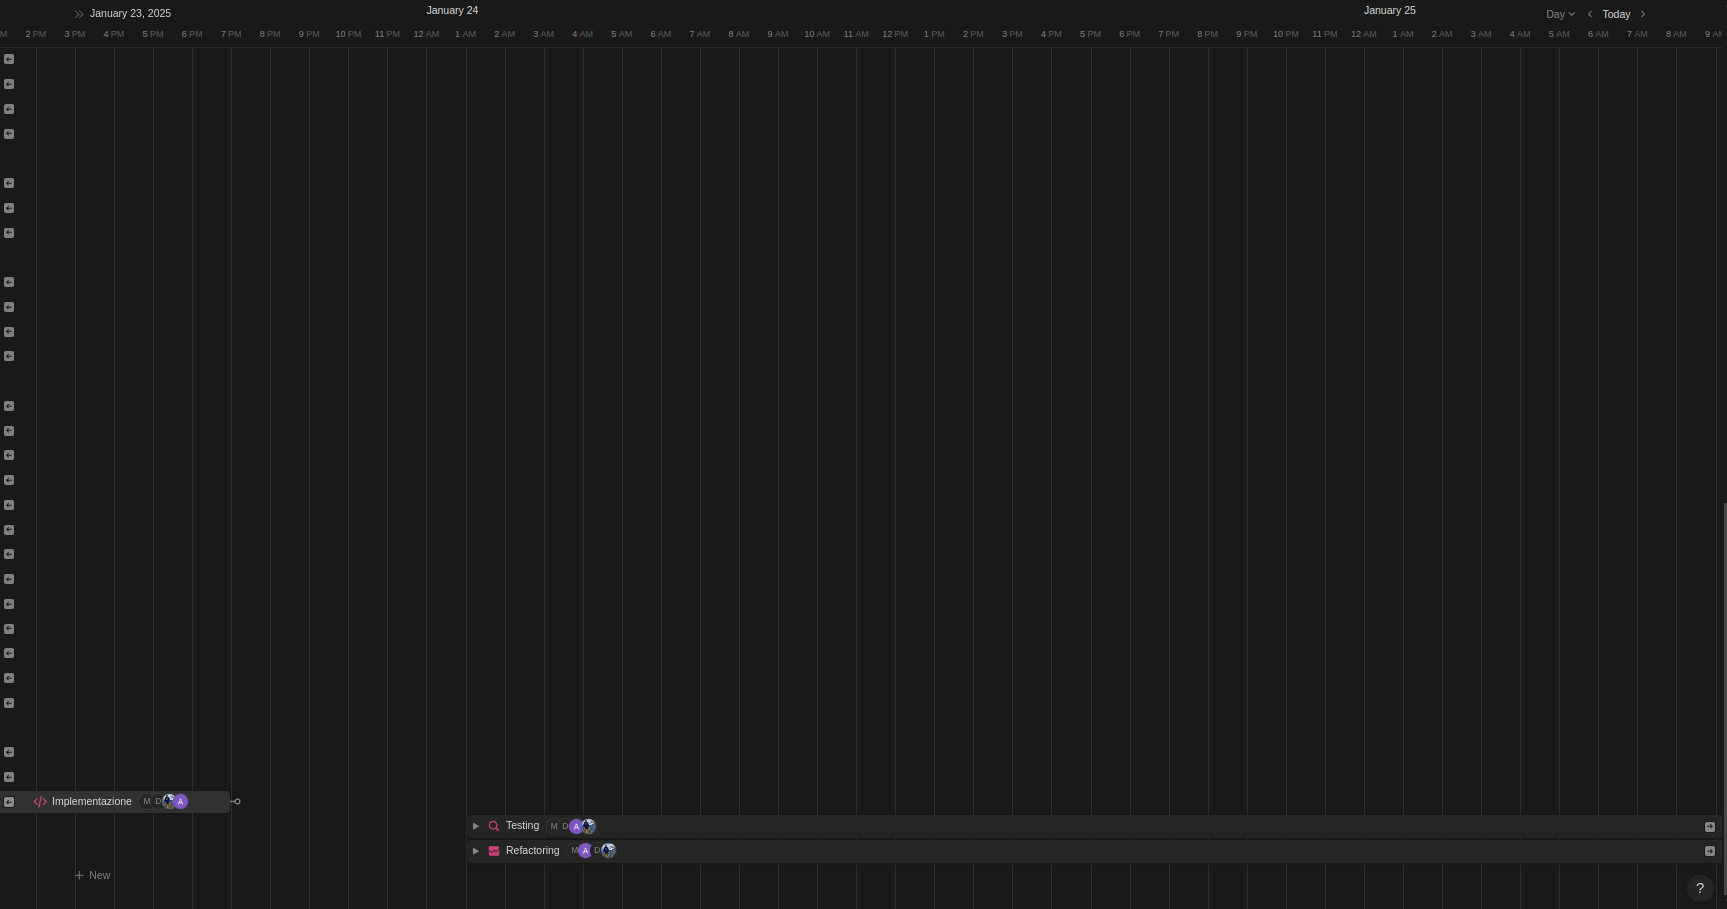
\includegraphics[width=\textwidth,keepaspectratio]{Immagini/Gantt/Iterazione 2/Gantt19.png}
        \caption{Diagramma di Gantt 19} 
        \label{fig:Gantt19}
\end{figure}

\begin{figure}[H]
    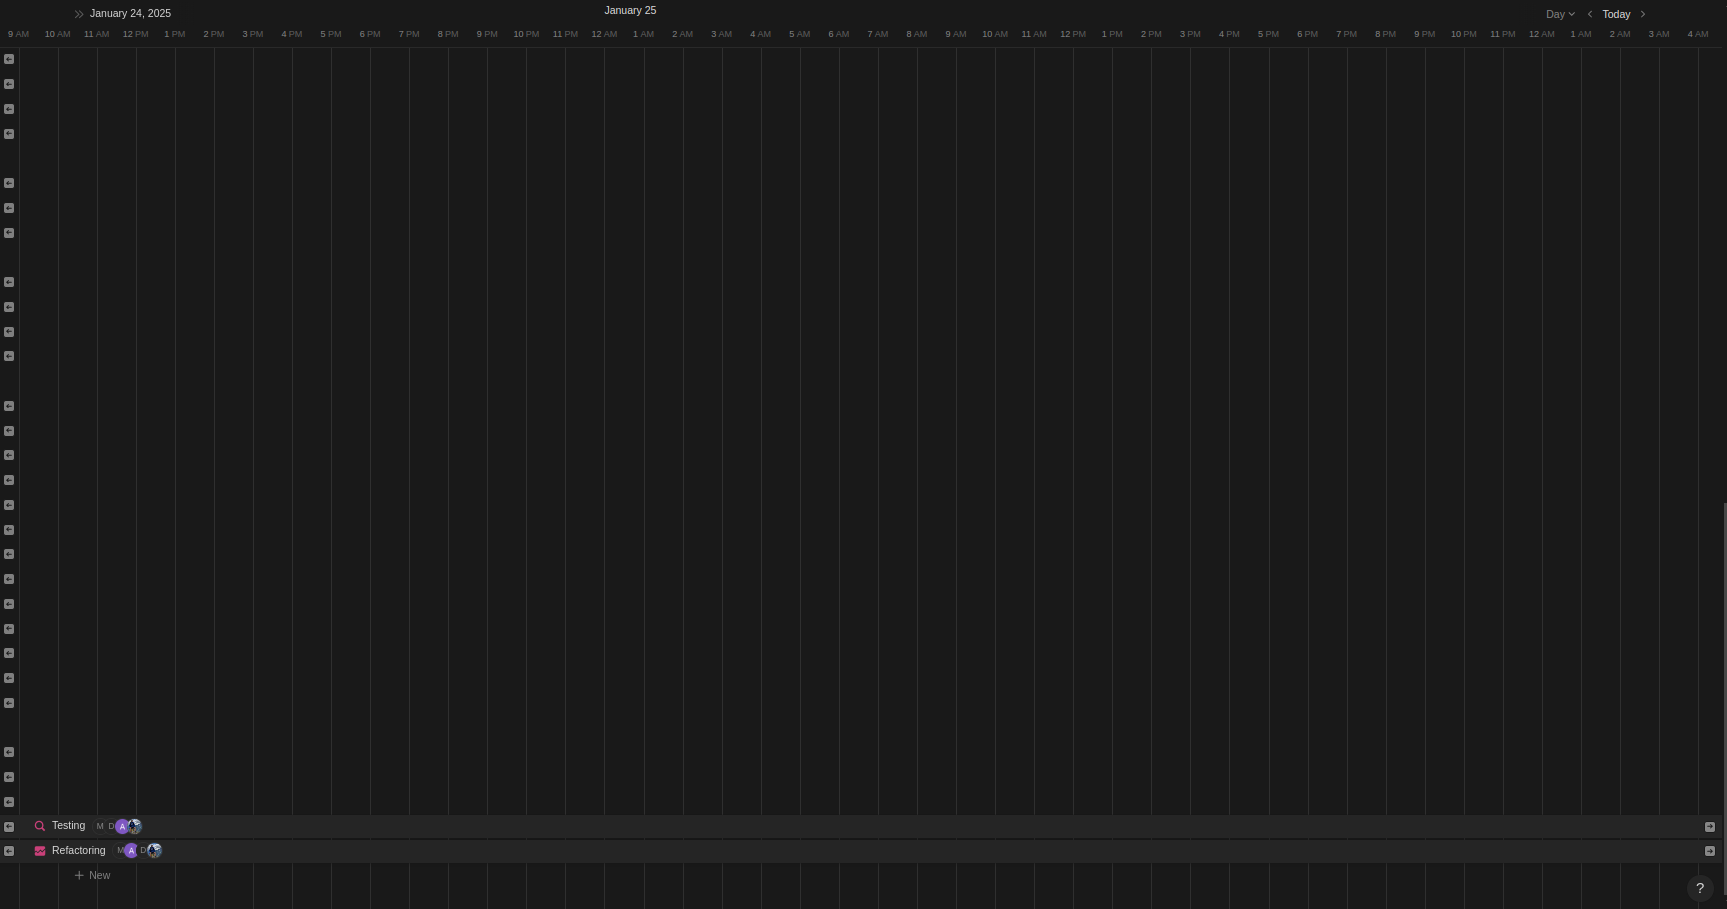
\includegraphics[width=\textwidth,keepaspectratio]{Immagini/Gantt/Iterazione 2/Gantt20.png}
        \caption{Diagramma di Gantt 20} 
        \label{fig:Gantt20}
\end{figure}

\begin{figure}[H]
    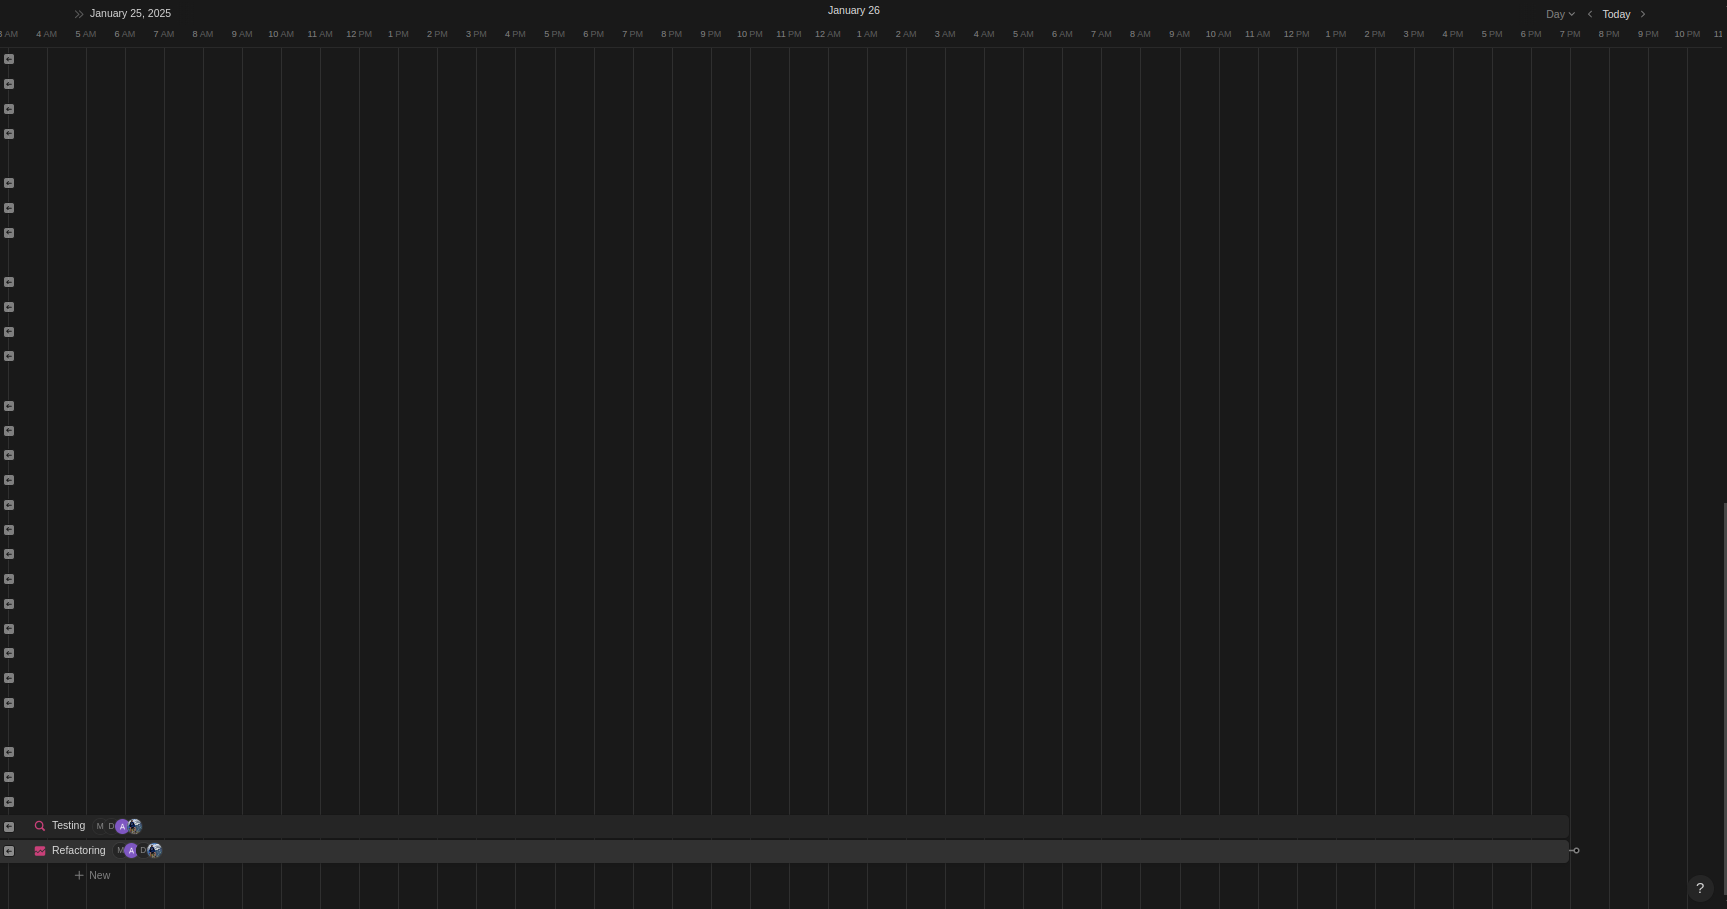
\includegraphics[width=\textwidth,keepaspectratio]{Immagini/Gantt/Iterazione 2/Gantt21.png}
        \caption{Diagramma di Gantt 21} 
        \label{fig:Gantt21}
\end{figure}

\section{Requisiti}

\subsection{Casi d'uso}

\subsubsection{Caso d'uso UC4: GestioneOfferteVolontariato}
\import{CasiD'uso/Iterazione 2/}{GestioneOfferteVolontariato.tex}

\subsubsection{Caso d'uso UC5: RicercaAbbinata}
\import{CasiD'uso/Iterazione 2/}{RicercaAbbinata.tex}

\subsection{Diagramma dei Casi d'Uso}
\import{Immagini/DiagrammaDeiCasiD'Uso/Iterazione 2/}{Diagramma.tex}
\begin{figure}[H]
    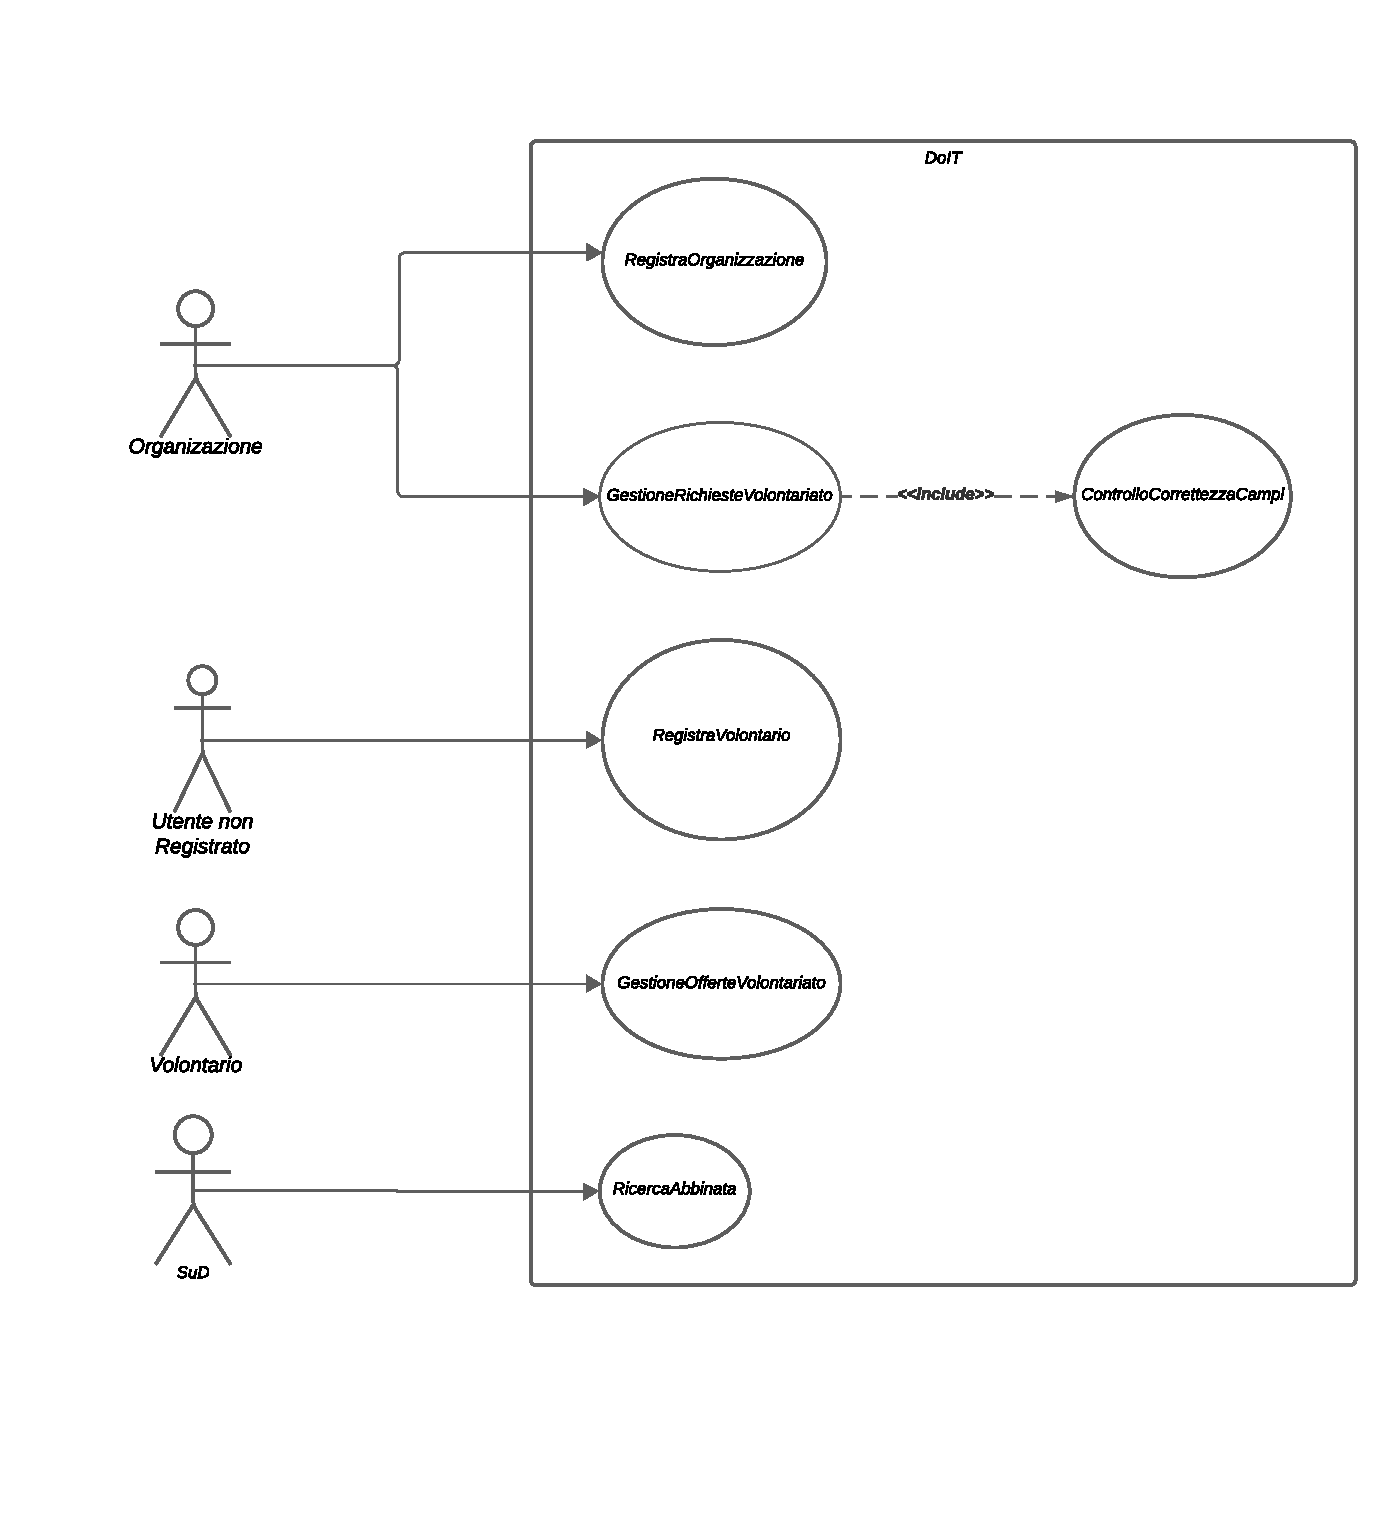
\includegraphics[width=\textwidth,keepaspectratio]{Immagini/DiagrammaDeiCasiD'Uso/Iterazione 2/Diagramma.pdf}
        \caption{Diagramma dei Casi d'Uso a seguito dell'iterazione 2}
        \label{fig:diagrammaCasiUso2}
\end{figure}

\subsection{Diagramma di Sequenza di Sistema}
\subsubsection{Diagramma di Sequenza di Sistema SSD4: GestioneOfferteVolontariato}
\import{Immagini/SSD/Iterazione 2/}{GestioneOfferteVolontariato.tex}

\begin{figure}[H]
    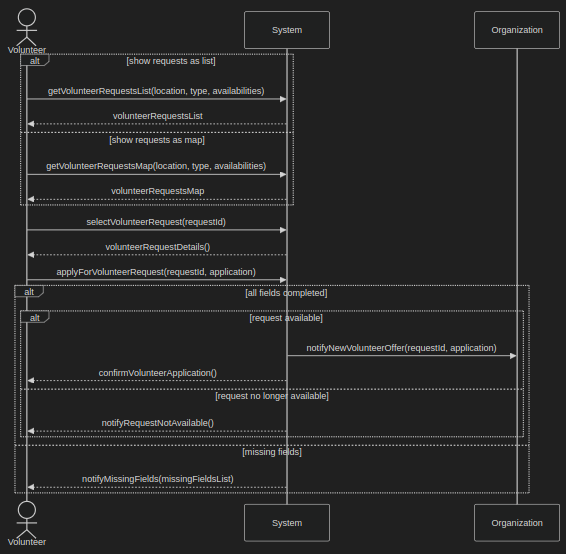
\includegraphics[width=\textwidth,keepaspectratio]{Immagini/SSD/Iterazione 2/SSDGestioneOfferteVolontariato.png}
        \caption{Diagramma di Sequenza di Sistema}
        \label{fig:diagrammaSSD4}
\end{figure}

\subsubsection{Diagramma di Sequenza di Sistema SSD5: RicercaAbbinata}
\import{Immagini/SSD/Iterazione 2/}{RicercaAbbinata.tex}

\begin{figure}[H]
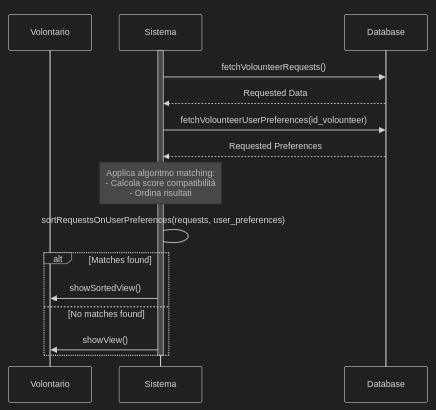
\includegraphics[width=\textwidth, keepaspectratio]{Immagini/SSD/Iterazione 2/SSDRicercaAbbinata.png}
        \caption{Diagramma di Sequenza di Sistema}
        \label{fig:diagrammaSSD5}
\end{figure}

\subsection{Contratti}
\subsubsection{Contratto CO03: RegistratiAdUnaRichiestaDiVolontariato}
\import{Contratti/Iterazione 2/}{RegistratiAdUnaRichiestaDiVolontariato.tex}

\subsubsection{Contratto CO04: OrdinaRichiesteSuPreferenzeUtente}
\import{Contratti/Iterazione 2/}{OrdinaRichiesteSuPreferenzeUtente.tex}

\subsection{Specifica Supplementare}
\textbf{Sono presenti solo i cambiamenti effettuati durante l'iterazione 2, i contenuti comuni non sono riscritti. Ciò che è stato rimosso presenta una cancellatura, ciò che è nuovo è sottoloneato}\\
\import{ArtefattiSupplementari/Iterazione 2/}{SpecificaSupplementare.tex}

\subsection{Glossario}
\textbf{Sono presenti solo i cambiamenti effettuati durante l'iterazione 2, i contenuti comuni non sono riscritti. Ciò che è stato rimosso presenta una cancellatura, ciò che è nuovo è sottoloneato}\\
\import{ArtefattiSupplementari/Iterazione 2/}{Glossario.tex}

\section{Modellazione di Business}

\subsection{Modello delle Classi Concettuali}
\import{Immagini/ModellazioneDiBusiness/Iterazione 2/}{Diagramma.tex}
\begin{figure}[H]
    \includegraphics[width=1.17\textwidth, height=\textheight,keepaspectratio]{Immagini/ModellazioneDiBusiness/Iterazione 2/Diagramma.png}
        \caption{Modello delle Classi Concettuali}
        \label{fig:Modello delle Classi Concettuali 2}
\end{figure}

\section{Progettazione}

\subsection{Diagrammi delle Classi Software di Progetto}

\subsubsection{Diagramma delle Classi Software di Progetto DCSP9: Dominio}
\import{Immagini/DCSP/Iterazione 2/}{Domain.tex}

\begin{figure}[H]
    \includegraphics[width=\textwidth, height=\textheight,keepaspectratio]{Immagini/DCSP/Iterazione 2/DCSPDomain.png}
        \caption{Diagramma delle Classi Software di Progetto}
        \label{fig:diagrammaDCSP9}
\end{figure}


\subsubsection{Diagramma delle Classi Software di Progetto DCSP10: Frontend}
\import{Immagini/DCSP/Iterazione 2/}{Frontend.tex}

\begin{figure}[H]
    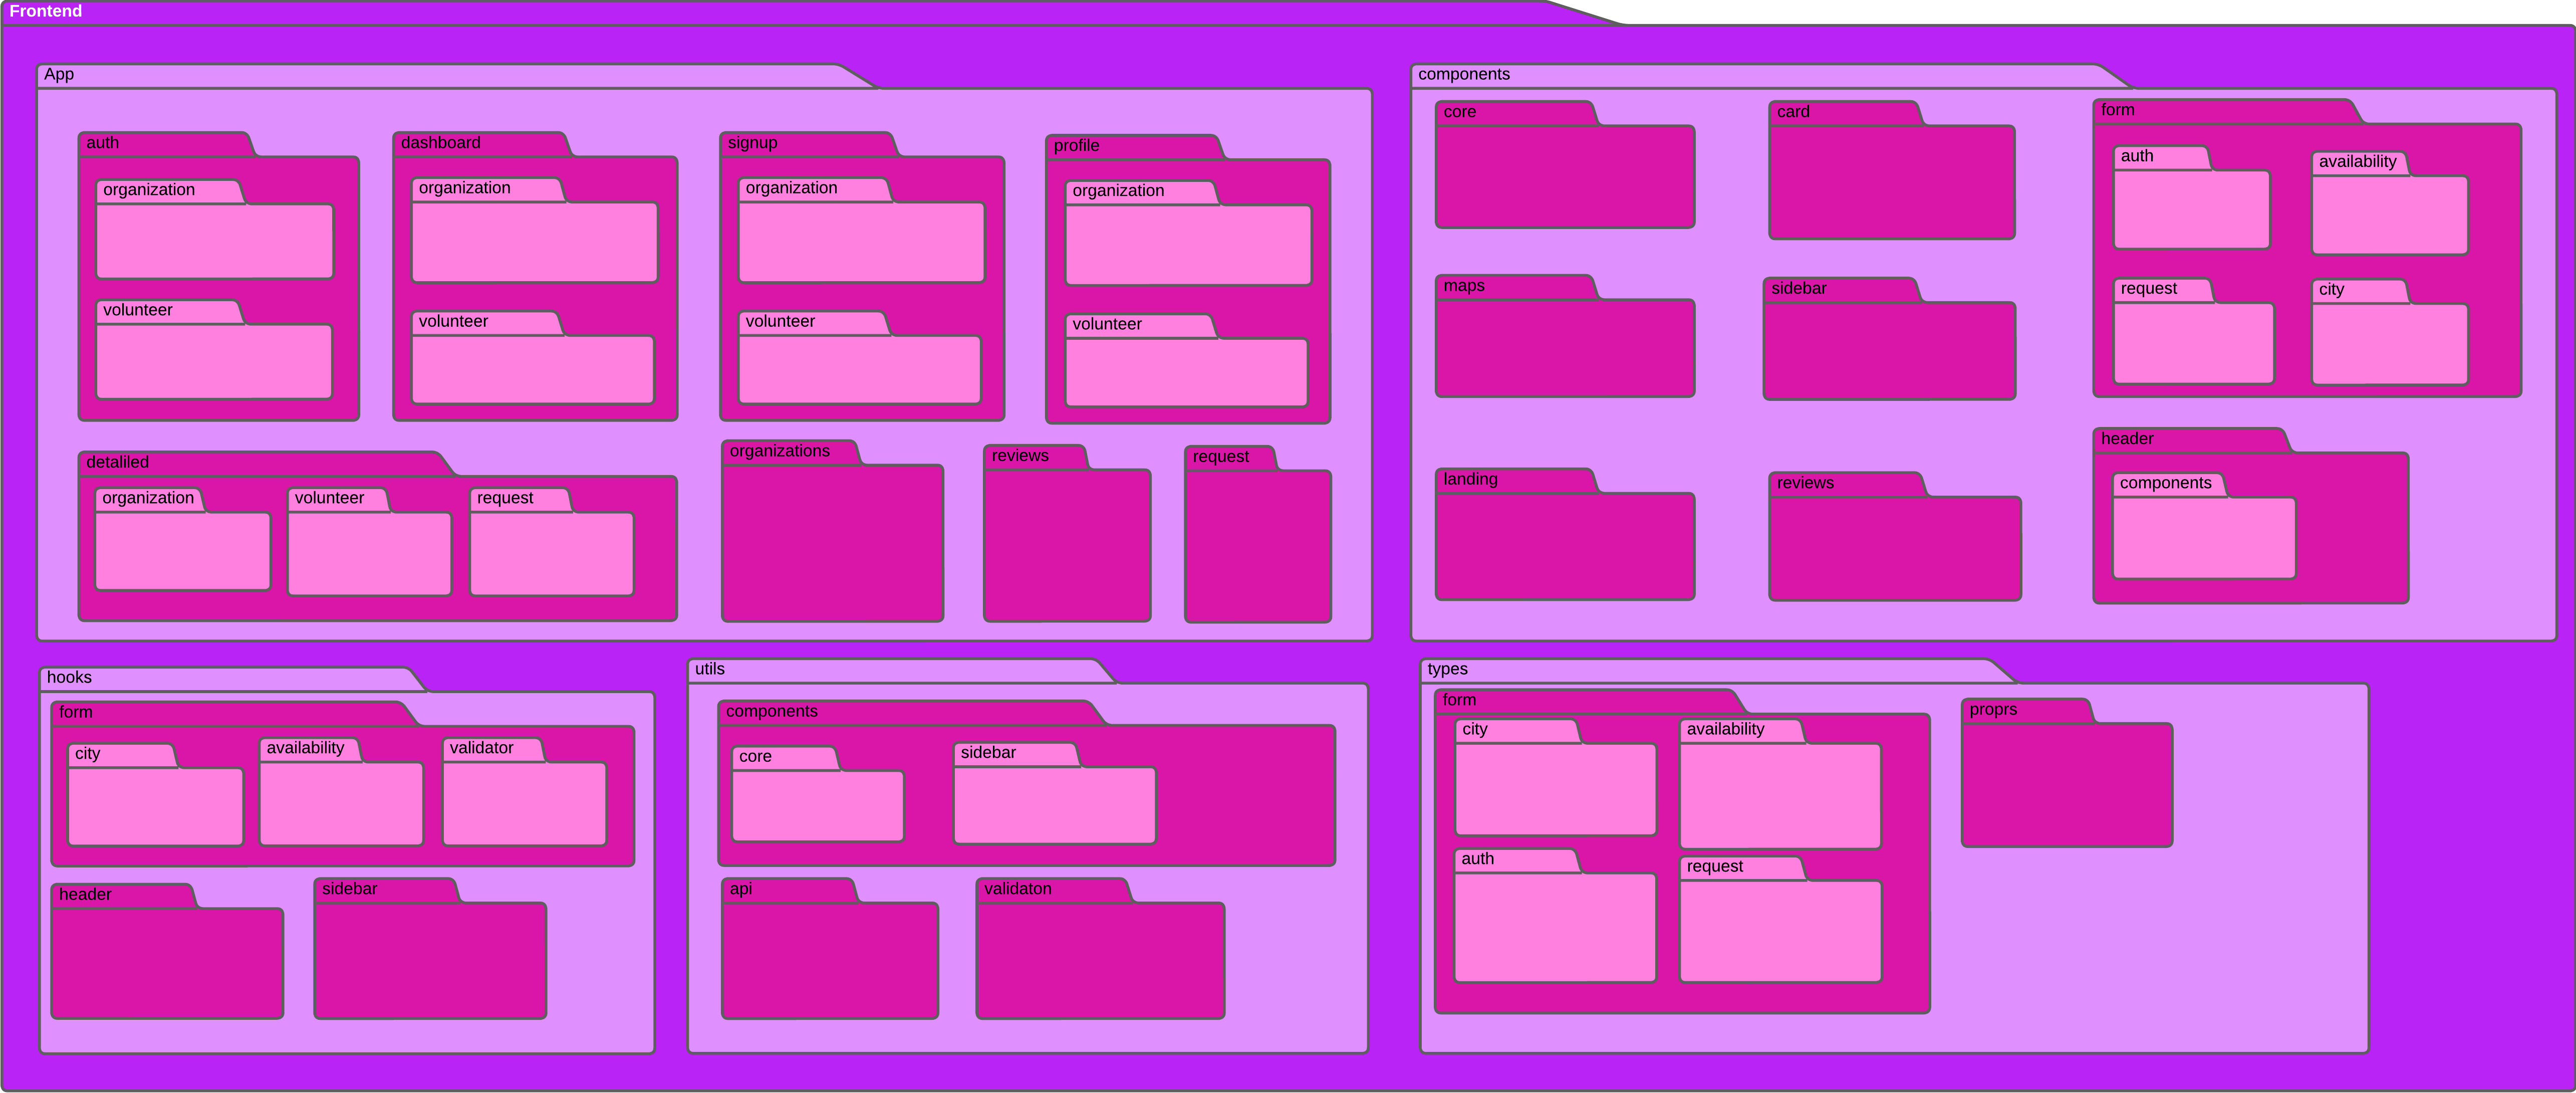
\includegraphics[width=\textwidth, height=\textheight,keepaspectratio]{Immagini/DCSP/Iterazione 2/DCSPFrontend.png}
        \caption{Diagramma delle Classi Software di Progetto}
        \label{fig:diagrammaDCSP10}
\end{figure}

\subsubsection{Diagramma delle Classi Software di Progetto DCSP11: Backend/Controller}
\import{Immagini/DCSP/Iterazione 2/Backend/}{Controller.tex}

\begin{figure}[H]
    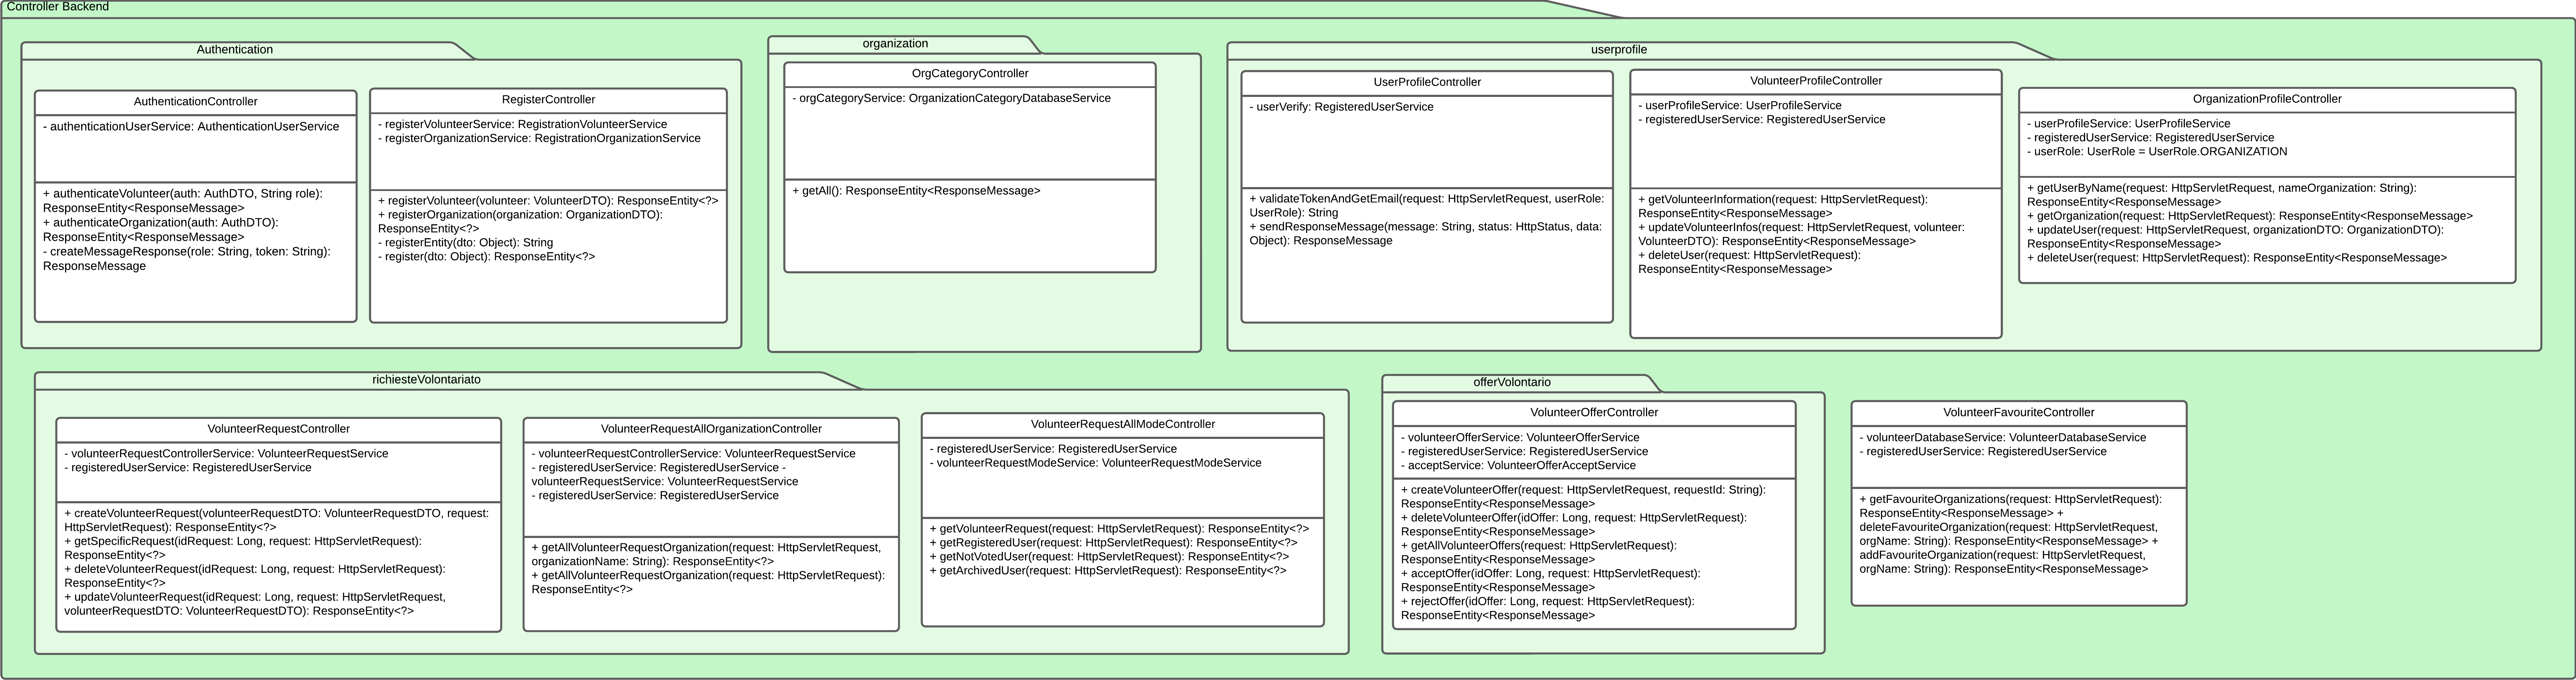
\includegraphics[width=\textwidth, height=\textheight,keepaspectratio]{Immagini/DCSP/Iterazione 2/Backend/DCSPController.png}
        \caption{Diagramma delle Classi Software di Progetto}
        \label{fig:diagrammaDCSP11}
\end{figure}

\subsubsection{Diagramma delle Classi Software di Progetto DCSP12: Backend/Domain}
\import{Immagini/DCSP/Iterazione 2/Backend/}{Domain.tex}

\begin{figure}[H]
    \includegraphics[width=\textwidth, height=\textheight,keepaspectratio]{Immagini/DCSP/Iterazione 2/Backend/DCSPDomain.png}
        \caption{Diagramma delle Classi Software di Progetto}
        \label{fig:diagrammaDCSP12}
\end{figure}

\subsubsection{Diagramma delle Classi Software di Progetto DCSP13: Backend/DTO}
\import{Immagini/DCSP/Iterazione 2/Backend/}{DTO.tex}

\begin{figure}[H]
    \includegraphics[width=\textwidth, height=\textheight,keepaspectratio]{Immagini/DCSP/Iterazione 2/Backend/DCSPDTO.png}
        \caption{Diagramma delle Classi Software di Progetto}
        \label{fig:diagrammaDCSP13}
\end{figure}

\subsubsection{Diagramma delle Classi Software di Progetto DCSP14: Backend/Mappers}
\import{Immagini/DCSP/Iterazione 2/Backend/}{Mappers.tex}

\begin{figure}[H]
    \includegraphics[width=\textwidth, height=\textheight,keepaspectratio]{Immagini/DCSP/Iterazione 2/Backend/DCSPMappers.png}
        \caption{Diagramma delle Classi Software di Progetto}
        \label{fig:diagrammaDCSP14}
\end{figure}

\subsubsection{Diagramma delle Classi Software di Progetto DCSP15: Backend/Service}
\import{Immagini/DCSP/Iterazione 2/Backend/}{Service.tex}

\begin{figure}[H]
    \includegraphics[width=\textwidth, height=\textheight,keepaspectratio]{Immagini/DCSP/Iterazione 2/Backend/DCSPService.png}
        \caption{Diagramma delle Classi Software di Progetto}
        \label{fig:diagrammaDCSP15}
\end{figure}

\subsubsection{Diagramma delle Classi Software di Progetto DCSP16: Backend/Repository}
\import{Immagini/DCSP/Iterazione 2/Backend/}{Repository.tex}

\begin{figure}[H]
    \includegraphics[width=\textwidth, height=\textheight,keepaspectratio]{Immagini/DCSP/Iterazione 2/Backend/DCSPRepository.png}
        \caption{Diagramma delle Classi Software di Progetto}
        \label{fig:diagrammaDCSP16}
\end{figure}

\subsection{Diagramma dell'Architettura Logica}

\subsubsection{Diagramma dell'Architettura Logica}
\import{Immagini/AL/Iterazione 2}{ArchitetturaLogica.tex}

\begin{figure}[H]
    \includegraphics[width=\textwidth, height=\textheight,keepaspectratio]{Immagini/AL/Iterazione 2/ALArchitetturaLogica.png}
        \caption{Diagramma dell'Architettura Logica}
        \label{fig:diagrammaAL2}
\end{figure}

\subsection{Pattern}
\import{Pattern/Iterazione 2/}{Introduzione.tex}

\subsubsection{Design Patterns}
\import{Pattern/Iterazione 2/}{Design Patterns.tex}


\subsubsection{Pattern Architetturali}
\import{Pattern/Iterazione 2/}{Pattern Architetturali.tex}


\subsubsection{Buone Pratiche}
\import{Pattern/Iterazione 2/}{Buone Pratiche.tex}

\subsubsection{Design Principles}
\import{Pattern/Iterazione 2/}{Design Principles.tex}

\section*{\Huge \textbf{Documenti dei Requisiti nella loro versione finale}}
\addcontentsline{toc}{section}{Artefatti Supplementari nella loro versione finale}
\setcounter{subsection}{0} 
\renewcommand{\thesubsection}{\arabic{subsection}} 

\subsection{Specifica Supplementare}
\import{ArtefattiSupplementari/}{SpecificaSupplementare.tex}

\subsection{Glossario}
\import{ArtefattiSupplementari/}{Glossario.tex}

\subsection{Visione}
\import{ArtefattiSupplementari/}{Visione.tex}

\section*{Understand}
\addcontentsline{toc}{section}{Understand}
\setcounter{subsection}{0} 
\renewcommand{\thesubsection}{\arabic{subsection}} 

\subsection{Analisi Generale}

\begin{figure}[H]
    \includegraphics[width=\textwidth, height=\textheight,keepaspectratio]{Immagini/Understand/Overall.png}
        \caption{Immagine dell'Analisi Generale}
        \label{fig:Understand1}
\end{figure}

\subsection{Metrics Treemaps}
Treemap che mostra le metriche \textbf{Countline: 90} e \textbf{CountLineCode: 75} individuate da Understand

\begin{figure}[H]
    \includegraphics[width=\textwidth, height=\textheight,keepaspectratio]{Immagini/Understand/Treemap.png}
        \caption{Immagine dell'Analisi sulle Linee di Codice}
        \label{fig:Understand2}
\end{figure}

\subsection{Metriche Generali}
\import{Immagini/Understand/}{Metrics.tex}

\subsection{Metriche del file: VolunteerRequestMatchingService}
\import{Immagini/Understand/}{VolunteerMetrics.tex}

\subsection{Conclusione}
\import{Immagini/Understand/}{Conclusione.tex}

\end{document}
